\documentclass[10pt,journal,compsoc]{IEEEtran}

% Some very useful LaTeX packages include:
% (uncomment the ones you want to load)


% *** MISC UTILITY PACKAGES ***
%
%\usepackage{ifpdf}
% Heiko Oberdiek's ifpdf.sty is very useful if you need conditional
% compilation based on whether the output is pdf or dvi.
% usage:
% \ifpdf
%   % pdf code
% \else
%   % dvi code
% \fi
% The latest version of ifpdf.sty can be obtained from:
% http://www.ctan.org/tex-archive/macros/latex/contrib/oberdiek/
% Also, note that IEEEtran.cls V1.7 and later provides a builtin
% \ifCLASSINFOpdf conditional that works the same way.
% When switching from latex to pdflatex and vice-versa, the compiler may
% have to be run twice to clear warning/error messages.






% *** CITATION PACKAGES ***
%
\ifCLASSOPTIONcompsoc
  % IEEE Computer Society needs nocompress option
  % requires cite.sty v4.0 or later (November 2003)
  \usepackage[nocompress]{cite}
\else
  % normal IEEE
  \usepackage{cite}
\fi
% cite.sty was written by Donald Arseneau
% V1.6 and later of IEEEtran pre-defines the format of the cite.sty package
% \cite{} output to follow that of IEEE. Loading the cite package will
% result in citation numbers being automatically sorted and properly
% "compressed/ranged". e.g., [1], [9], [2], [7], [5], [6] without using
% cite.sty will become [1], [2], [5]--[7], [9] using cite.sty. cite.sty's
% \cite will automatically add leading space, if needed. Use cite.sty's
% noadjust option (cite.sty V3.8 and later) if you want to turn this off
% such as if a citation ever needs to be enclosed in parenthesis.
% cite.sty is already installed on most LaTeX systems. Be sure and use
% version 5.0 (2009-03-20) and later if using hyperref.sty.
% The latest version can be obtained at:
% http://www.ctan.org/tex-archive/macros/latex/contrib/cite/
% The documentation is contained in the cite.sty file itself.
%
% Note that some packages require special options to format as the Computer
% Society requires. In particular, Computer Society  papers do not use
% compressed citation ranges as is done in typical IEEE papers
% (e.g., [1]-[4]). Instead, they list every citation separately in order
% (e.g., [1], [2], [3], [4]). To get the latter we need to load the cite
% package with the nocompress option which is supported by cite.sty v4.0
% and later. Note also the use of a CLASSOPTION conditional provided by
% IEEEtran.cls V1.7 and later.





% *** GRAPHICS RELATED PACKAGES ***
%
\ifCLASSINFOpdf
    \usepackage[pdftex]{graphicx}
  % declare the path(\bm{s}) where your graphic files are
    \graphicspath{{./pics/}}
  % and their extensions so you won't have to specify these with
  % every instance of \includegraphics
  %  \DeclareGraphicsExtensions{.pdf,.jpeg,.png}
\else
  % or other class option (dvipsone, dvipdf, if not using dvips). graphicx
  % will default to the driver specified in the system graphics.cfg if no
  % driver is specified.
  % \usepackage[dvips]{graphicx}
  % declare the path(\bm{s}) where your graphic files are
  % \graphicspath{{../eps/}}
  % and their extensions so you won't have to specify these with
  % every instance of \includegraphics
  % \DeclareGraphicsExtensions{.eps}
\fi
% graphicx was written by David Carlisle and Sebastian Rahtz. It is
% required if you want graphics, photos, etc. graphicx.sty is already
% installed on most LaTeX systems. The latest version and documentation
% can be obtained at:
% http://www.ctan.org/tex-archive/macros/latex/required/graphics/
% Another good source of documentation is "Using Imported Graphics in
% LaTeX2e" by Keith Reckdahl which can be found at:
% http://www.ctan.org/tex-archive/info/epslatex/
%
% latex, and pdflatex in dvi mode, support graphics in encapsulated
% postscript (.eps) format. pdflatex in pdf mode supports graphics
% in .pdf, .jpeg, .png and .mps (metapost) formats. Users should ensure
% that all non-photo figures use a vector format (.eps, .pdf, .mps) and
% not a bitmapped formats (.jpeg, .png). IEEE frowns on bitmapped formats
% which can result in "jaggedy"/blurry rendering of lines and letters as
% well as large increases in file sizes.
%
% You can find documentation about the pdfTeX application at:
% http://www.tug.org/applications/pdftex






% *** MATH PACKAGES ***
%
\usepackage[cmex10]{amsmath}
% A popular package from the American Mathematical Society that provides
% many useful and powerful commands for dealing with mathematics. If using
% it, be sure to load this package with the cmex10 option to ensure that
% only type 1 fonts will utilized at all point sizes. Without this option,
% it is possible that some math symbols, particularly those within
% footnotes, will be rendered in bitmap form which will result in a
% document that can not be IEEE Xplore compliant!
%
% Also, note that the amsmath package sets \interdisplaylinepenalty to 10000
% thus preventing page breaks from occurring within multiline equations. Use:
\interdisplaylinepenalty=2500
% after loading amsmath to restore such page breaks as IEEEtran.cls normally
% does. amsmath.sty is already installed on most LaTeX systems. The latest
% version and documentation can be obtained at:
% http://www.ctan.org/tex-archive/macros/latex/required/amslatex/math/





% *** SPECIALIZED LIST PACKAGES ***
%
%\usepackage{algorithmic}
% algorithmic.sty was written by Peter Williams and Rogerio Brito.
% This package provides an algorithmic environment fo describing algorithms.
% You can use the algorithmic environment in-text or within a figure
% environment to provide for a floating algorithm. Do NOT use the algorithm
% floating environment provided by algorithm.sty (by the same authors) or
% algorithm2e.sty (by Christophe Fiorio) as IEEE does not use dedicated
% algorithm float types and packages that provide these will not provide
% correct IEEE style captions. The latest version and documentation of
% algorithmic.sty can be obtained at:
% http://www.ctan.org/tex-archive/macros/latex/contrib/algorithms/
% There is also a support site at:
% http://algorithms.berlios.de/index.html
% Also of interest may be the (relatively newer and more customizable)
% algorithmicx.sty package by Szasz Janos:
% http://www.ctan.org/tex-archive/macros/latex/contrib/algorithmicx/




% *** ALIGNMENT PACKAGES ***
%
\usepackage{array}
% Frank Mittelbach's and David Carlisle's array.sty patches and improves
% the standard LaTeX2e array and tabular environments to provide better
% appearance and additional user controls. As the default LaTeX2e table
% generation code is lacking to the point of almost being broken with
% respect to the quality of the end results, all users are strongly
% advised to use an enhanced (at the very least that provided by array.sty)
% set of table tools. array.sty is already installed on most systems. The
% latest version and documentation can be obtained at:
% http://www.ctan.org/tex-archive/macros/latex/required/tools/


% IEEEtran contains the IEEEeqnarray family of commands that can be used to
% generate multiline equations as well as matrices, tables, etc., of high
% quality.




% *** SUBFIGURE PACKAGES ***
\ifCLASSOPTIONcompsoc
  \usepackage[caption=false,font=footnotesize,labelfont=sf,textfont=sf]{subfig}
\else
  \usepackage[caption=false,font=footnotesize]{subfig}
\fi
% subfig.sty, written by Steven Douglas Cochran, is the modern replacement
% for subfigure.sty, the latter of which is no longer maintained and is
% incompatible with some LaTeX packages including fixltx2e. However,
% subfig.sty requires and automatically loads Axel Sommerfeldt's caption.sty
% which will override IEEEtran.cls' handling of captions and this will result
% in non-IEEE style figure/table captions. To prevent this problem, be sure
% and invoke subfig.sty's "caption=false" package option (available since
% subfig.sty version 1.3, 2005/06/28) as this is will preserve IEEEtran.cls
% handling of captions.
% Note that the Computer Society format requires a sans serif font rather
% than the serif font used in traditional IEEE formatting and thus the need
% to invoke different subfig.sty package options depending on whether
% compsoc mode has been enabled.
%
% The latest version and documentation of subfig.sty can be obtained at:
% http://www.ctan.org/tex-archive/macros/latex/contrib/subfig/




% *** FLOAT PACKAGES ***
%
\usepackage{fixltx2e}
% fixltx2e, the successor to the earlier fix2col.sty, was written by
% Frank Mittelbach and David Carlisle. This package corrects a few problems
% in the LaTeX2e kernel, the most notable of which is that in current
% LaTeX2e releases, the ordering of single and double column floats is not
% guaranteed to be preserved. Thus, an unpatched LaTeX2e can allow a
% single column figure to be placed prior to an earlier double column
% figure. The latest version and documentation can be found at:
% http://www.ctan.org/tex-archive/macros/latex/base/


%\usepackage{stfloats}
% stfloats.sty was written by Sigitas Tolusis. This package gives LaTeX2e
% the ability to do double column floats at the bottom of the page as well
% as the top. (e.g., "\begin{figure*}[!b]" is not normally possible in
% LaTeX2e). It also provides a command:
%\fnbelowfloat
% to enable the placement of footnotes below bottom floats (the standard
% LaTeX2e kernel puts them above bottom floats). This is an invasive package
% which rewrites many portions of the LaTeX2e float routines. It may not work
% with other packages that modify the LaTeX2e float routines. The latest
% version and documentation can be obtained at:
% http://www.ctan.org/tex-archive/macros/latex/contrib/sttools/
% Do not use the stfloats baselinefloat ability as IEEE does not allow
% \baselineskip to stretch. Authors submitting work to the IEEE should note
% that IEEE rarely uses double column equations and that authors should try
% to avoid such use. Do not be tempted to use the cuted.sty or midfloat.sty
% packages (also by Sigitas Tolusis) as IEEE does not format its papers in
% such ways.
% Do not attempt to use stfloats with fixltx2e as they are incompatible.
% Instead, use Morten Hogholm'a dblfloatfix which combines the features
% of both fixltx2e and stfloats:
%
% \usepackage{dblfloatfix}
% The latest version can be found at:
% http://www.ctan.org/tex-archive/macros/latex/contrib/dblfloatfix/




%\ifCLASSOPTIONcaptionsoff
%  \usepackage[nomarkers]{endfloat}
% \let\MYoriglatexcaption\caption
% \renewcommand{\caption}[2][\relax]{\MYoriglatexcaption[#2]{#2}}
%\fi
% endfloat.sty was written by James Darrell McCauley, Jeff Goldberg and
% Axel Sommerfeldt. This package may be useful when used in conjunction with
% IEEEtran.cls'  captionsoff option. Some IEEE journals/societies require that
% submissions have lists of figures/tables at the end of the paper and that
% figures/tables without any captions are placed on a page by themselves at
% the end of the document. If needed, the draftcls IEEEtran class option or
% \CLASSINPUTbaselinestretch interface can be used to increase the line
% spacing as well. Be sure and use the nomarkers option of endfloat to
% prevent endfloat from "marking" where the figures would have been placed
% in the text. The two hack lines of code above are a slight modification of
% that suggested by in the endfloat docs (section 8.4.1) to ensure that
% the full captions always appear in the list of figures/tables - even if
% the user used the short optional argument of \caption[]{}.
% IEEE papers do not typically make use of \caption[]'s optional argument,
% so this should not be an issue. A similar trick can be used to disable
% captions of packages such as subfig.sty that lack options to turn off
% the subcaptions:
% For subfig.sty:
% \let\MYorigsubfloat\subfloat
% \renewcommand{\subfloat}[2][\relax]{\MYorigsubfloat[]{#2}}
% However, the above trick will not work if both optional arguments of
% the \subfloat command are used. Furthermore, there needs to be a
% description of each subfigure *somewhere* and endfloat does not add
% subfigure captions to its list of figures. Thus, the best approach is to
% avoid the use of subfigure captions (many IEEE journals avoid them anyway)
% and instead reference/explain all the subfigures within the main caption.
% The latest version of endfloat.sty and its documentation can obtained at:
% http://www.ctan.org/tex-archive/macros/latex/contrib/endfloat/
%
% The IEEEtran \ifCLASSOPTIONcaptionsoff conditional can also be used
% later in the document, say, to conditionally put the References on a
% page by themselves.




% *** PDF, URL AND HYPERLINK PACKAGES ***
%
%\usepackage{url}
% url.sty was written by Donald Arseneau. It provides better support for
% handling and breaking URLs. url.sty is already installed on most LaTeX
% systems. The latest version and documentation can be obtained at:
% http://www.ctan.org/tex-archive/macros/latex/contrib/url/
% Basically, \url{my_url_here}.





% *** Do not adjust lengths that control margins, column widths, etc. ***
% *** Do not use packages that alter fonts (such as pslatex).         ***
% There should be no need to do such things with IEEEtran.cls V1.6 and later.
% (Unless specifically asked to do so by the journal or conference you plan
% to submit to, of course. )

\usepackage{enumitem}
%\usepackage[]{algorithm2e}
\usepackage[]{algpseudocode}
\usepackage{algorithm}
\usepackage{multirow}
\usepackage{slashbox}
\usepackage{color}
%\usepackage[numbers,sort&compress]{natbib}
%\usepackage{ulem}
\renewcommand{\arraystretch}{1.3}

\usepackage{color}
\usepackage{bm}
%\usepackage{mathrsfs}
\usepackage[mathcal]{eucal}
\usepackage{amsfonts}
\usepackage{amssymb}
\usepackage{wrapfig}

\usepackage{amsthm}

\usepackage{amssymb}% http://ctan.org/pkg/amssymb
\usepackage{pifont}% http://ctan.org/pkg/pifont
\newcommand{\cmark}{\ding{51}}%
\newcommand{\xmark}{\ding{55}}%
% correct bad hyphenation here
\hyphenation{op-tical net-works semi-conduc-tor}

\newcommand{\tabincell}[2]{\begin{tabular}{@{}#1@{}}#2\end{tabular}}

\floatname{algorithm}{Algorithm}
%\usepackage[utf8]{inputenc}
\usepackage[english]{babel}
\newtheorem{theorem}{Theorem}

\begin{document}
\title{Efficient and Robust Boolean Operations on N Meshes Based on Hybrid Representations}
\author{%Rui~Wang,~
        %Xudong~Jiang,~
        %Hongbo~Fu,~
        %Ping~Li,~
        %Bin~Sheng~and
        %Enhua~Wu
\IEEEcompsocitemizethanks{

\IEEEcompsocthanksitem R. Wang and B. Sheng are with the Department of Computer Science and Engineering, Shanghai Jiao Tong University. Email:\{jhcz,shengbin\}@sjtu.edu.cn

\IEEEcompsocthanksitem X. Jiang is with Autodesk China Research \& Development Center. Email: xudong.jiang@autodesk.com

\IEEEcompsocthanksitem H. Fu is with the School of Creative Media, City University of Hong Kong. Email: hongbofu@cityu.edu.hk

\IEEEcompsocthanksitem P. Li is with the Department of Mathematics and Information Technology, The Hong Kong Institute of Education. Email: pli@ied.edu.hk

\IEEEcompsocthanksitem E. Wu is currently a research professor at State Key Lab. of Computer Science, Institute of Software, Chinese Academy of Sciences. Email: ehwu@umac.mo}
}

%\markboth{Journal of \LaTeX\ Class Files,~Vol.~13, No.~9, September~2014}%
%{Shell \MakeLowercase{\textit{et al.}}: Bare Demo of IEEEtran.cls for Computer Society Journals}




\IEEEtitleabstractindextext{
\begin{abstract}
  Constructive solid geometry (CSG) is a widely used modeling tool. It constructs complex models by combining primitive solids with boolean operations. However, boolean evaluation, which computes the final model of CSG, has suffered from robustness problem for more than three decades. Some methods are fast but not robust, while some methods are robust but rely on exact arithmetic which is slow. Recent works tried to implement fast and robust boolean evaluation methods using plane-based representations (P-reps) of polyhedrons instead of vertex-based representations (V-reps) of polyhedrons. While they have achieved remarkable improvements, they are still slow compared with non-robust methods. We propose a fast and robust boolean method. It uses hybrid representations of polyhedrons, which combines P-reps with V-reps. It allows us to take advantages of both the efficiency of V-reps and the exactness of P-reps. Comparison experiments with the state-of-the-art show that our method is unconditionally robust for solid inputs, and is similarly efficient to existing non-robust methods.
\end{abstract}


\begin{IEEEkeywords}
boolean operations, CSG evaluation, plane-based geometry
\end{IEEEkeywords}

}

\maketitle


\IEEEdisplaynontitleabstractindextext
\IEEEpeerreviewmaketitle


\IEEEraisesectionheading{\section{Introduction}\label{sec:introduction}}
\IEEEPARstart{C}{onstructive} solid geometry (CSG) has long been a popular modeling tool for computer-aided design and computer-aided manufacturing (CAD / CAM). Complex models are constructed by combining primitives using regularized boolean operations \cite{requicha1977mathematical,tilove1980closure}: union, intersection, and difference. A CSG can be converted into the boundary representation (B-rep) through boolean evaluation. There are two major types of boolean evaluation methods, which vary according to how they deal with intersections between primitives.
Approximate methods \cite{wang2011approximate,pavic2010hybrid,biermann2001approximate} rediscretize the intersection areas, fit vertices approximatively, and rearrange the topology.
Conversely, exact methods \cite{ogayar2015deferred,douze2015quickcsg,zhou2016mesh} do not change vertex positions, and maintain as many input elements (such as faces, vertices, and topology) as possible. In many applications, exact methods are preferred for their accuracy. Additionally, the clear mapping between the surfaces of the input and output meshes in exact methods simplifies the inheritance of surface information, such as face colors and materials.



However, there is always a compromise between robustness and efficiency for exact boolean algorithms.
Robust methods often require exact arithmetic \cite{barki2015exact,zhou2016mesh}, which is significantly slower than normal floating-point arithmetic.
Other methods only guarantee \textbf{quasi-robust} \cite{shewchuk1999lecture} by using unreliable techniques, such as epsilon-tweaking \cite{laidlaw1986constructive,feito2013fast,segal1990using} and numerical perturbation \cite{douze2015quickcsg}.
Recently, robust plane-based methods have been developed \cite{bernstein2009fast,campen2010exact} based on binary space partition (BSP) merging algorithms \cite{naylor1990merging,thibault1987set}.
The robustness of these methods is guaranteed by the theorem of Sugihara and Iri \cite{sugihara1990solid} that boolean evaluations can be performed without \textbf{constructions} \cite{shewchuk1999lecture} if polyhedrons are represented based on planes instead of vertices.
By only use \textbf{predicates}, boolean methods are easier to be robust.
These plane-based methods are generally faster than others which using exact arithmetic. However, they still suffer from performance issues because of the high computation complexity of BSP algorithms. In addition, the incoherence between BSP representations and B-reps of polyhedrons requires that extra steps for conversion and connectivity reconstruction, leading to worse performance.


Inspired by these previous studies, we develop a robust boolean method, which is unconditionally robust given consistent solid inputs, and as fast as non-robust methods. In our method, we combine P-reps with V-reps, forming hybrid representations of solids. Generally, the V-reps information is used for coarse tests and efficient neighboring face queries, while P-reps information is used for exact predicates. To avoid using exact arithmetic and ensure efficiency, we avoid constructions throughout our method.


Our method is different from the previous BSP-based methods \cite{bernstein2009fast,campen2010exact}.
While their methods are largely based on BSP theorem of \cite{naylor1990merging,thibault1987set}, our method is more like vertex-based methods such as \cite{feito2013fast,zhou2016mesh} and is significantly faster than these BSP-based methods. Our method is not a simple improvement of vertex-based methods, but a systematical solution for robustness of boolean evaluations. During intersection computation, we encode the triangle intersections into sets of planes, and then use these planes to determine exact tessellations. Subsequently, we classify each face in the tessellated meshes using small local BSP trees, which also compliment the P-reps to guarantee exactness. In order to guarantee performance, we try to minimize the usage of plane-based exact predicates in these stages. In addition, while most existing boolean methods can only process two meshes, our method is \textbf{variadic} \cite{zhou2016mesh}, which can evaluate arbitrary inputs immediately. Thus, our method may reduce evaluation time of large CSGs by avoiding repetitive computation. Experiments have shown that our method is much faster than existing robust methods, and only around two times slower than non-robust methods.

\section{Related Work}


Boolean methods have been researched since their inception in the 1980s \cite{requicha1985boolean, laidlaw1986constructive}. Existing methods can be put into two categories: exact methods and approximate methods. Exact methods retain vertex positions, and the topology of the inputs is preserved as much as possible. The coordinates of intersection points between input meshes are computed by input configurations. However, the coordinates cannot be represented exactly using fixed-precision floating point numbers, hence exact arithmetic is needed for robustness. Conversely, approximate methods rediscretize the input mesh surfaces using techniques such as voxels, octrees, and Layered Depth Images (LDI). These methods generally have better performance and easier to be robust than exact methods, but the loss of precision and geometry information is inevitable. In this section, we first introduce previous work of these two categories, and then discuss plane-based boolean methods, which have close relation with our method.

\subsection{Exact Methods}


Some exact methods \cite{ogayar2015deferred,douze2015quickcsg,xu2013fast,feito2013fast,updegrove2016boolean}, are optimized for efficiency, but cannot guarantee robustness. They are implemented by fixed-precision floating-point arithmetic, so numerical errors are inevitable, which often leads to inconsistent results.
Douze et al. \cite{douze2015quickcsg} developed a very efficient method for handling very large meshes and arbitrary input primitives. However, this method makes general position assumption and cannot deal with coplanar situations.


Many researchers have attempted to solve the robustness issues using arbitrary precision arithmetic \cite{banerjee1996topologically, fortune1995polyhedral, keyser2004esolid, granados2003boolean, hachenberger2005boolean, zhou2016mesh,barki2015exact} and exact interval computation \cite{fang1993robustness, hu1996robust, segal1990using}. However, these methods are too expensive in terms of computation time. For example, CGAL's \cite{cgal:hk-bonp3-15a} exact-arithmetic implementation \cite{granados2003boolean} of Nef polyhedra \cite{bieri1988elementary} is more than 50 times slower than non-robust boolean operations \cite{bernstein2009fast}.



\subsection{Approximative Methods}


Because it is difficult to achieve efficiency, accuracy, and robustness simultaneously, some methods sacrifice accuracy for greater efficiency and robustness. Most such methods are based on volumetric representations of meshes. However, the quality of the resulting mesh depends on the resolution of the volume grid, and better quality requires significantly higher resolutions.
To accelerate this process, some methods reduce the complexity of the output mesh \cite{varadhan2004topology}, whereas others preserve non-intersected areas of the input mesh to avoid redundant tessellation \cite{pavic2010hybrid,wang2011approximate,zhao2011parallel,hable2005blister,ogayar2006gpu,updegrove2016boolean}.
Moreover, with the development of general-purpose computing on graphics processing units (GPGPU), many of them utilize the computational power of graphics hardware for boolean evaluations. These methods have good performance, and are suitable for interactive applications. However, the fundamental problem of approximate methods arises from the grid-dependent nature of volumetric calculations. They inevitably suffer from geometric detail loss and unwieldy topological changes.


\subsection{Plane-Based Methods}
\label{sec:pbrelated}

The concept of plane-based representations (P-reps) of polyhedrons was first described by Sugihara and Iri \cite{sugihara1990solid}. By using P-reps, boolean evaluations can be performed with only predicates, which are much easier to implement robustly. Berstein and Fussell \cite{bernstein2009fast} combined P-reps with BSP trees \cite{thibault1987set,naylor1990merging} to develop a boolean method which is unconditionally robust with consistent inputs. Unlike vertex-based methods, their method does not rely on exact arithmetic to be robust.
However, the merging of two BSP trees is has $O(mn)$ time complexity, where $m$ and $n$ are the size of the trees. Such high time complexity makes this method impractical for large meshes. Subsequently, Campen and Kobbelt \cite{campen2010exact} improved this method by localizing BSP operations using an octree. In this method, mesh refinements only take place locally near intersections, which leads to better performance. However, their method splits the intersection regions and non-intersection regions, and requires extra stitching step to reconstruct topology. Also, the performance of localized BSP merging is still poor compared with the vertex-based methods.


\section{Background and Overview}

\label{sec:overview}

Our method is designed for boolean evaluations on arbitrary number of inputs primitives \cite{requicha1985boolean}. Primitives are triangular solid meshes free of self-intersecting. Geometry connectivity is also required as inputs. Even if there are topological deficiencies, our method still try to give acceptable answer. Our method is not sensitive to topological deficiencies which are not near the regions where primitives intersect.

In the following, we first discuss the causes of non-robustness of boolean methods. Then we analyze the cause of inefficiency of previous plane-based methods and discuss how to avoid these problems. Finally, we give an overview of the proposed method.


\subsection{Robustness of Boolean Methods}
\label{sec:paradigm}

The boolean evaluations on mesh primitives are, in essence, a process of face selection. Namely, given a boolean expression, the operation collect those faces that satisfy the expression to generate the final mesh. Whether a certain face $\bm{s}$ belong to the final mesh is determined by its inclusion labels and the boolean expression $f$:
\begin{equation}
\lambda_f(\bm{s}) = f(\boldsymbol{\Lambda}(\bm{s})) = f(\lambda_1(\bm{s}), \lambda_2(\bm{s}), \cdots, \lambda_n(\bm{s})),
\end{equation}
where $\lambda_i(\bm{s})$ is the inclusion label with respect to primitive $M_i$. Each label has four conditions: completely inside (\emph{in}), completely outside (\emph{out}), on the boundary with consistent normal vector (\emph{same}) or with opposite normal vector (\emph{oppo}). To compute $\lambda_f(\bm{s})$, the labels with respect to all of the primitives (as $\boldsymbol{\Lambda}(\bm{s})$) must be known.
The evaluation of boolean expression with inclusion labels are discussed in \cite{douze2015quickcsg,feito2013fast}. If and only if $\lambda_f(\bm{s})=same$, $\bm{s}$ is on the surface of the final mesh.

Unfortunately, not all of the input faces can be classified collectively. For some faces near the intersections, only parts of them belong to the final mesh. Therefore, an extra step before face classification is required to detect intersections between meshes. Then input meshes are tessellated according to these intersections to ensure that every face is completely inside, outside, or on the boundary of other input meshes.

Most of the existing boolean methods follow such two-step paradigm---intersection computation and face classification, as does our method. Non-robustness comes from three stages of such boolean methods. 1) The intersection between faces may not be exactly computed. 2) Face tessellation produces inconsistent topology. 3) The computation of the inclusion labels is not consistent with the location of the faces (see Fig. \ref{fig:falseclass}). These problems all come from the numerical errors during geometric computation. Therefore, if these three stages can be performed in exact ways, boolean evaluations are robust.

\begin{figure}[t]
\centering
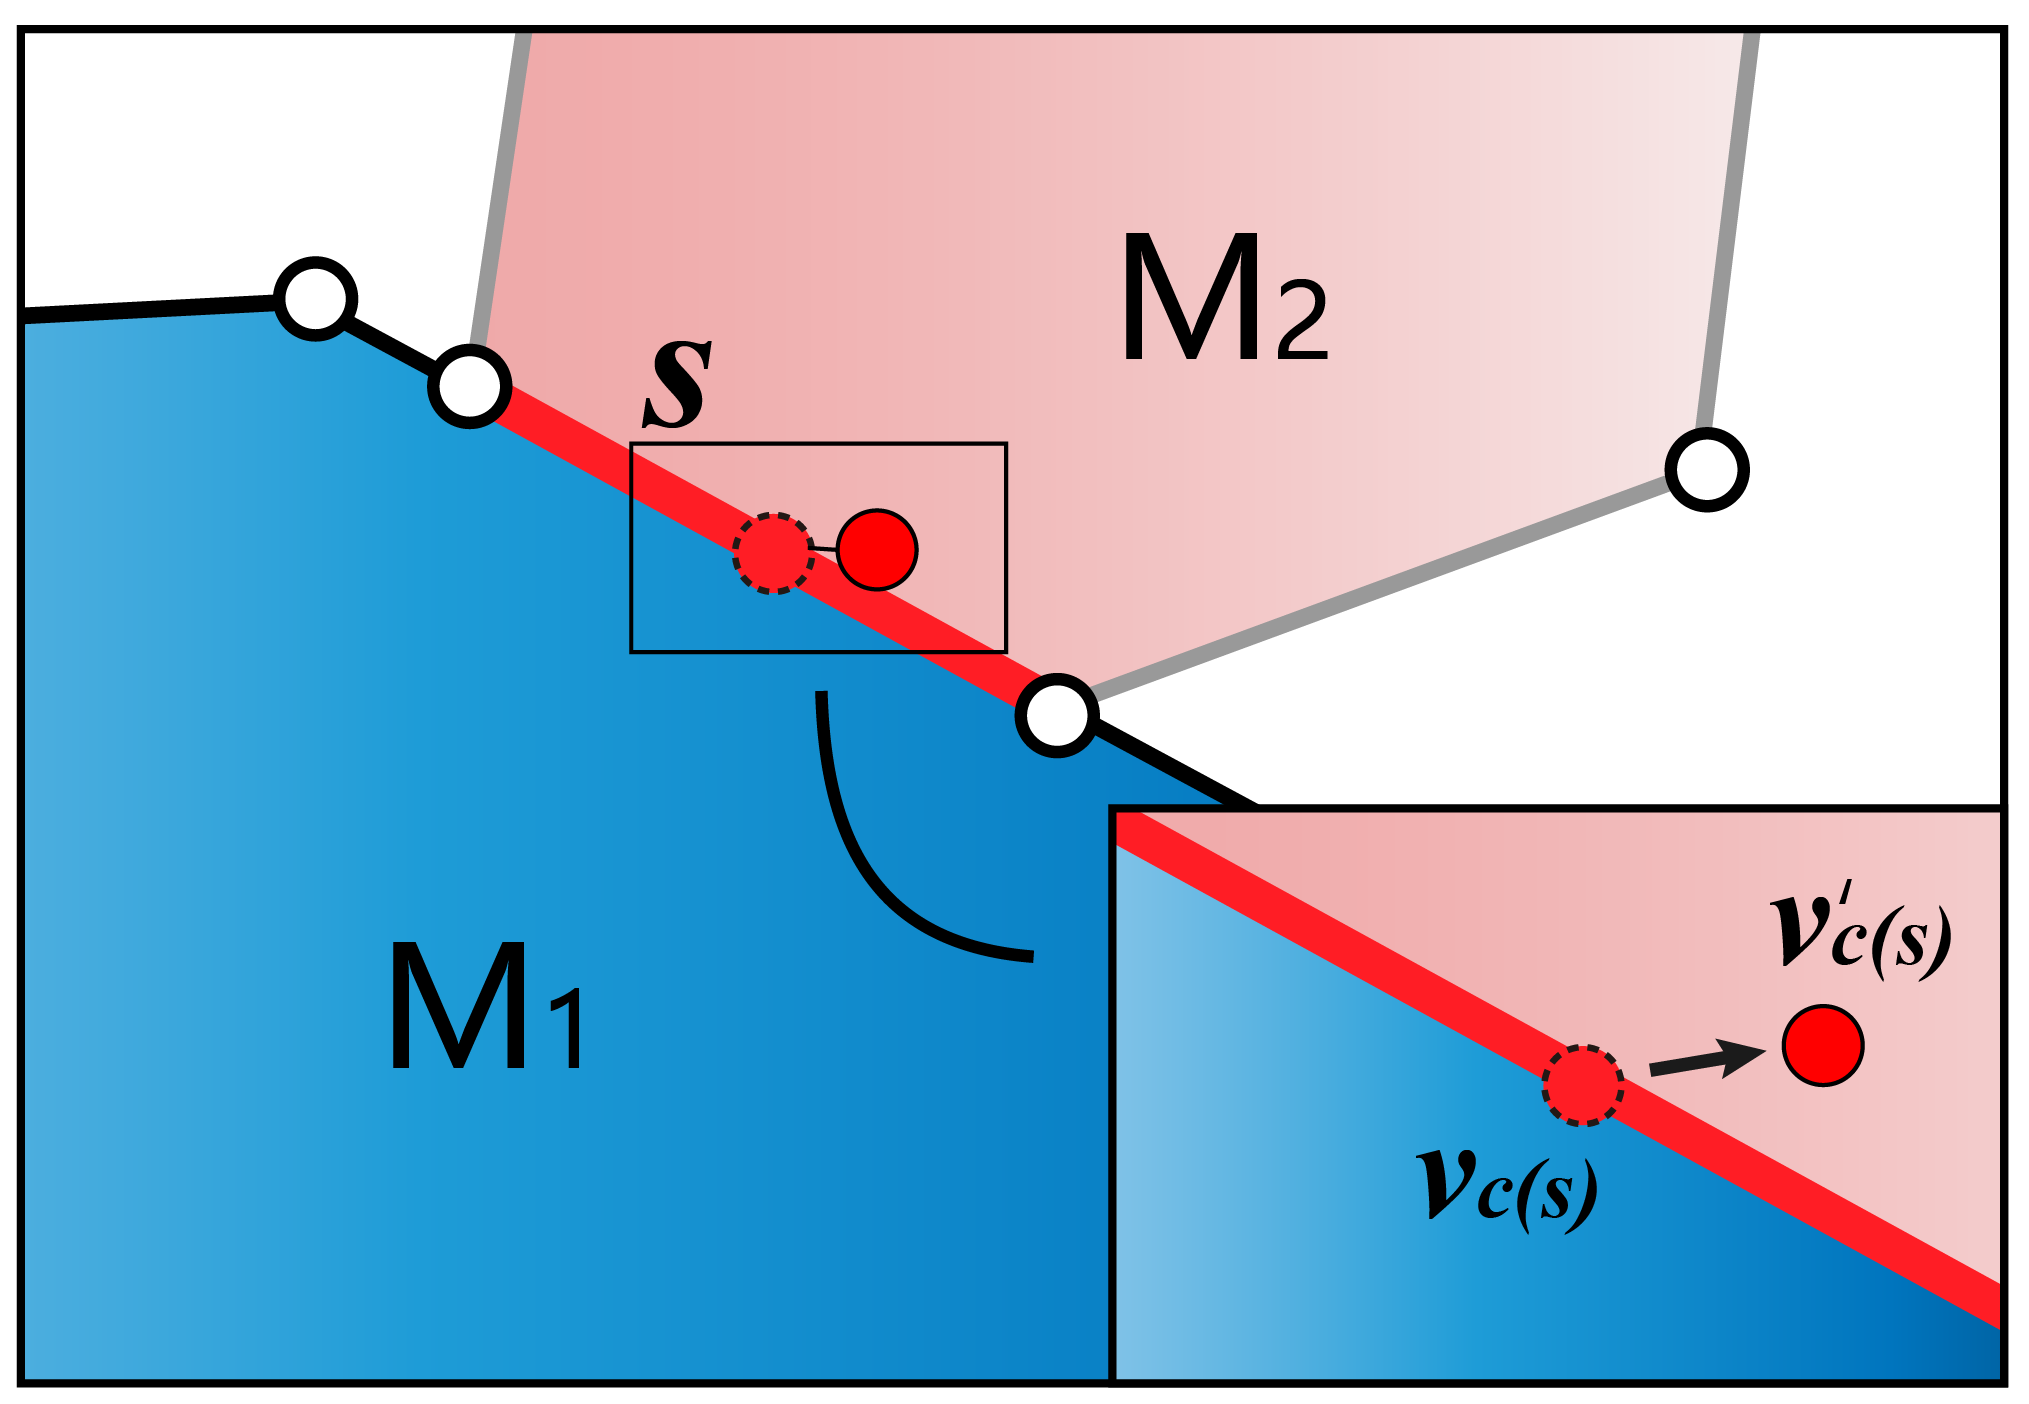
\includegraphics[width=2.2in]{boolean-01}
\caption{In this 2D view, face $\bm{s}$ (the red line segment) of mesh $M_2$ is on the surface of mesh $M_1$. However, because the face barycenter $\bm{v}_{c(\bm{s})}$ is used to compute the labels, the coordinates of which contain round-off errors, the point could be moved to $\bm{v'}_{c(\bm{s})}$. Thus, $\bm{s}$ may be falsely classified as being outside of $M_1$.}
\label{fig:falseclass}
\end{figure}


\subsection{Plane-based booleans}
Comparing with applying exact arithmetic, using plane-based geometry \cite{campen2010exact} is more promising to produce efficient exact computations. Therefore, in our method, we use P-reps as the key to avoid numerical errors.

\label{sec:substrates}
\subsubsection{Plane-based representation}


\begin{wrapfigure}{r}[0in]{0in}
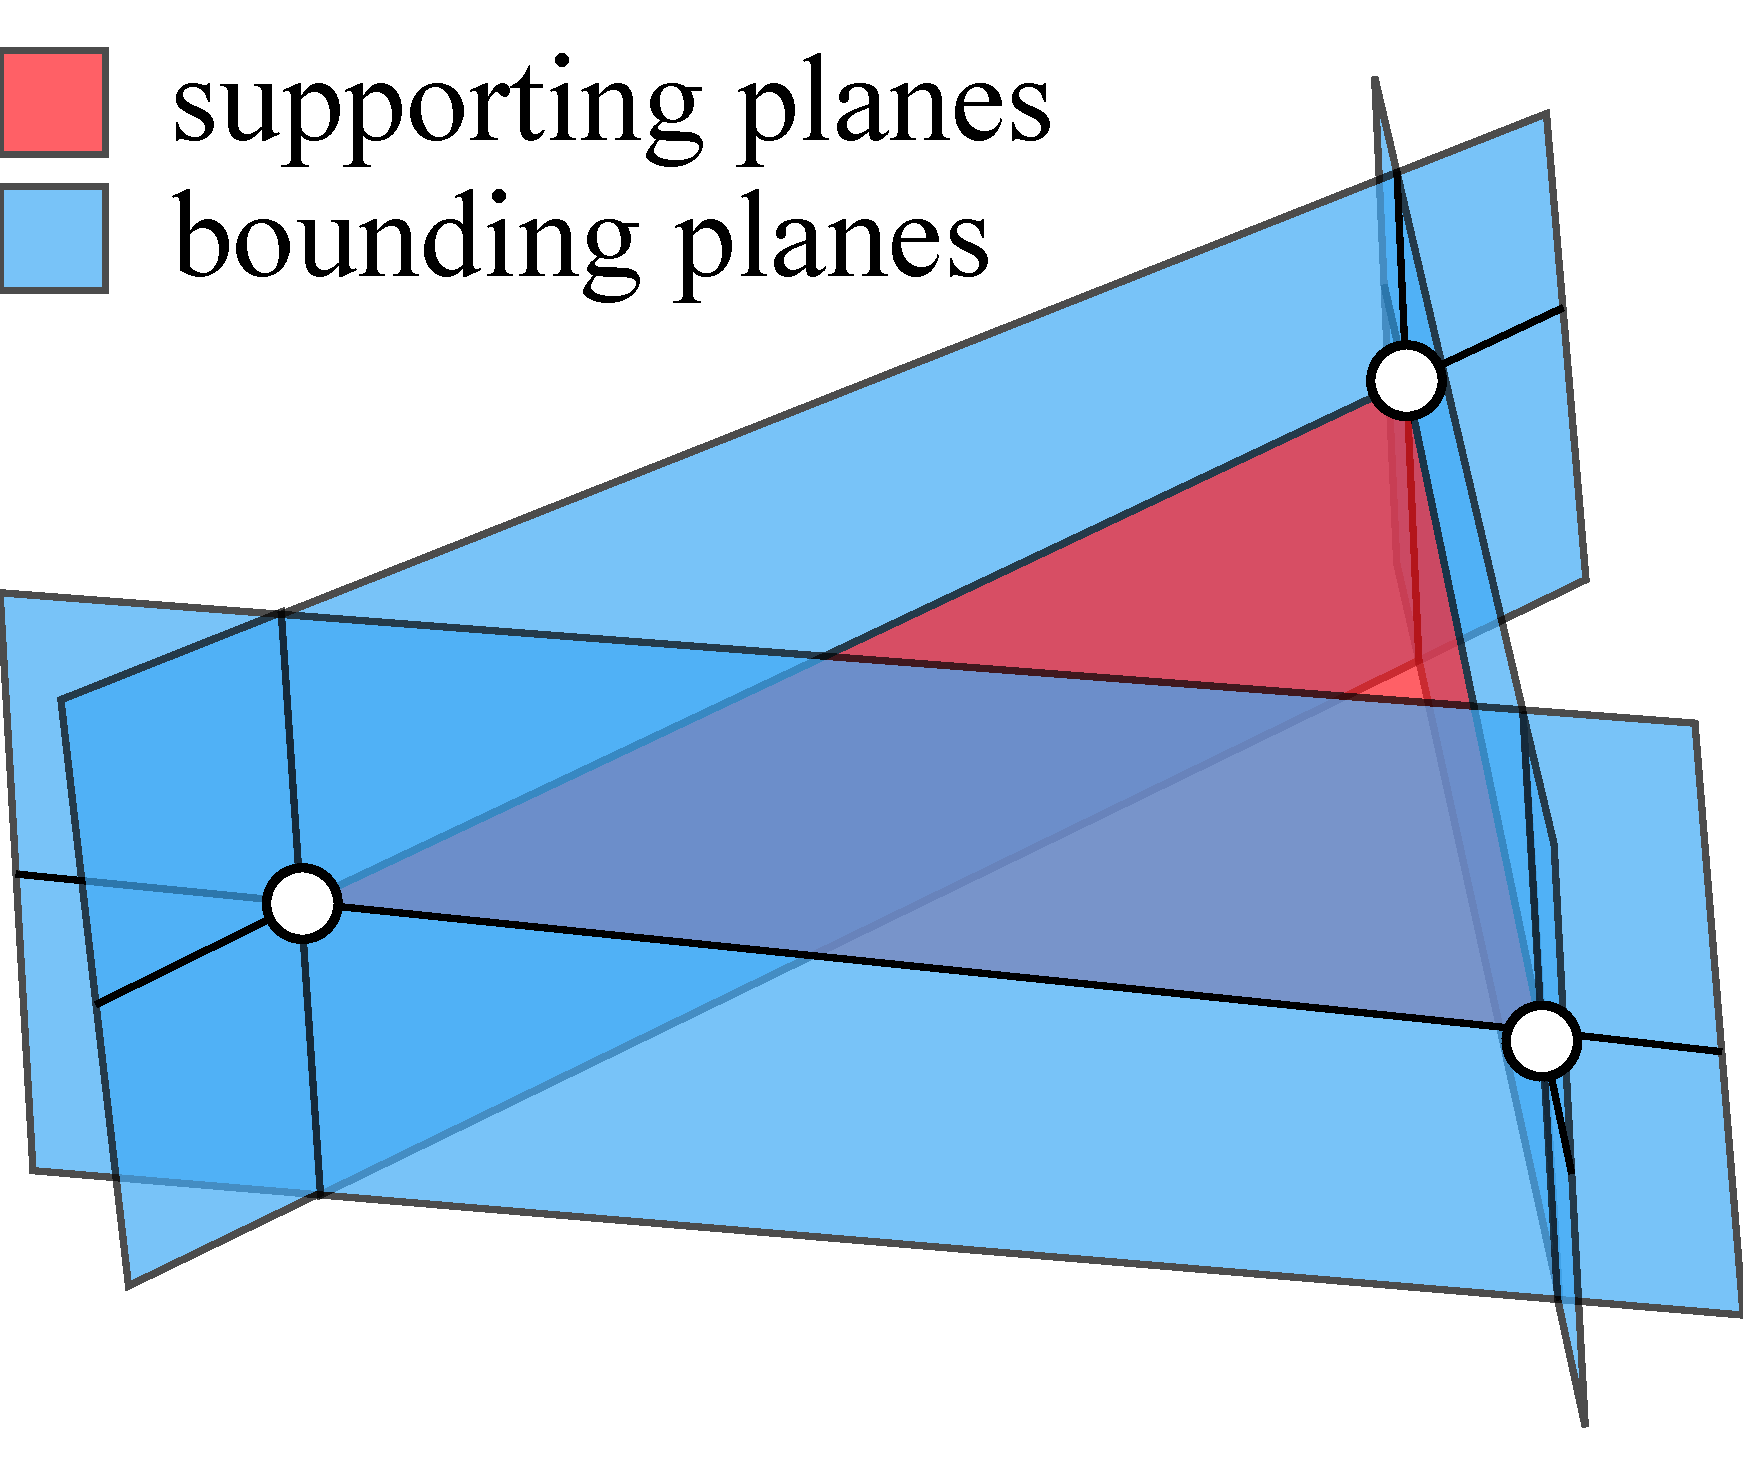
\includegraphics[width=1.5 in]{p-reps}
\end{wrapfigure}

Using P-reps, each face $\bm{s}$ with $n$ edges is represented by a supporting plane $\bm{p}_{s,sp}$ on which the face lies, and a set bounding planes $\{\bm{p}_{s,b}^i \ \vert\  i = 0, 1,...,n-1\}$. Each edge line $\bm{e}_{\bm{s}}^i$ is represented by the intersection $\bm{p}_{s,sp} \cap \bm{p}_{s,b}^i$.
Vertex $\bm{v}_s^i$ is represented by the intersection of $\bm{p}_{s,sp}$ and two consecutive bounding planes. We use the method of Campen et al. \cite{campen2010exact} for the exact conversion of triangles to their P-reps. The exact plane-based predicates are sped up using numerical filtering techniques by Shewchuk \cite{shewchuk1997adaptive}.


Other commonly used notations in this paper are presented below. The normal of a plane $\bm{p}$ is denoted as $\bm{n}(\bm{p})$. A line $\bm{l}$ of P-reps can be represented by the intersection of two planes $(\bm{p}_l^0 \cap \bm{p}_l^1)$, hence, $\bm{l}\colon(\bm{p}_l^0 \cap \bm{p}_l^1)$. The positive direction of the line $\bm{l}$ is defined by $\bm{n}(\bm{p}_l^0) \times \bm{n}(\bm{p}_l^1)$.
A point $\bm{v}$ of P-reps can be represented by non-trivial plane triples $(\bm{p}_v^0 \cap \bm{p}_v^1 \cap \bm{p}_v^2)$, hence, $\bm{v}\colon(\bm{p}_v^0 \cap \bm{p}_v^1 \cap \bm{p}_v^2)$.

\subsubsection{Efficient embedding}

Under P-reps, vertex is represented with a much higher precision than under V-reps. A plane is represented by four parameters. Then a vertex takes twelve parameters under P-reps compared with only three parameters under V-reps. This makes geometric computations significantly slower under P-reps. Even though numerical filters can be applied to speed up, pure plane-based methods, such as \cite{sugihara1990solid,banerjee1996topologically}, cannot be as fast as vertex-based methods. On the other hand, a hybrid representation may bring both the efficiency of V-reps and the exactness of P-reps. And plane-based geometric computation should be avoided as much as possible to reduce computation cost.

BSP-based boolean algorithms are substantially based on planes, therefore are suitable to implement with P-reps \cite{bernstein2009fast,campen2010exact}. However, BSP merging is a pure plane-based algorithm. Also, BSP structure has additional two drawbacks which make it slow: a) BSP algorithms have high time complexity. b) BSP structure destroy geometry connectivity information, thus algorithms benefiting from connectivity require extra effort to reconstruct connectivity. Therefore, as an exact but not efficient representation, BSP should not substitute V-reps in total, but can serve as a compliment of V-reps to help plane-based geometric computation. Also, BSP structure has to be localized to minimize its size.

In our method, we use V-reps for coarse tests and fast connectivity queries and P-reps for exact predicates. The framework of our method is based on \cite{ogayar2015deferred}, which is a vertex-based method. Plane-based algorithms are embedded into the processing. This embedding is not a simple plane-based implementation of vertex-based algorithms. We develop three efficient algorithms which is optimized under P-reps: triangle-triangle intersection tests, triangle tessellation and polygon classification. These three algorithms are corresponding to the three sources of non-robustness discussed in \S\ref{sec:paradig}. The major difficulty is to avoid any computation under high precision, which means our method is designed to be implemented using only common double-precision floating-point arithmetic. Though BSP-based methods \cite{bernstein2009fast,campen2010exact} also do not use high precision arithmetic, this constrain is harder to satisfy under a vertex-based framework.


\subsubsection{Mapping to three diemensions}

Many vertex-based algorithms, such as 2D triangulation and face classification, is hard to implement under P-reps because they requires projection from three dimensions to planes or lines.  Projections are performed on vertex coordinates which are absent under P-reps. Since plane-based predicates \cite{bernstein2009fast,banerjee1996topologically} are usually performed under three dimensions, we have to find the equivalent three dimensional problem, whose projection to low dimension is the problem we want to compute. In the following, we discuss three such plane-based algorithms used in our method.

\vspace{0.5em}
\noindent \textbf{Point-line orientation}

\noindent Within the plane $\bm{p}_0$, the point-line orientation is computed by the line parameters and point coordinates under V-reps. Under P-reps, we map this problem to point-plane orientation by picking a plane $\bm{p_l}$ which satisfy three requirements: 1) the line is in $\bm{p_l}$. 2) $\bm{p_l}$ is not parallel with $\bm{p}_0$. 3) $\bm{n}(\bm{p}_0) \times \bm{n}(\bm{p_l})$ has the same orientation as the line.

\vspace{0.5em}
\noindent \textbf{Linear ordering of points}

\begin{figure}
  \centering
  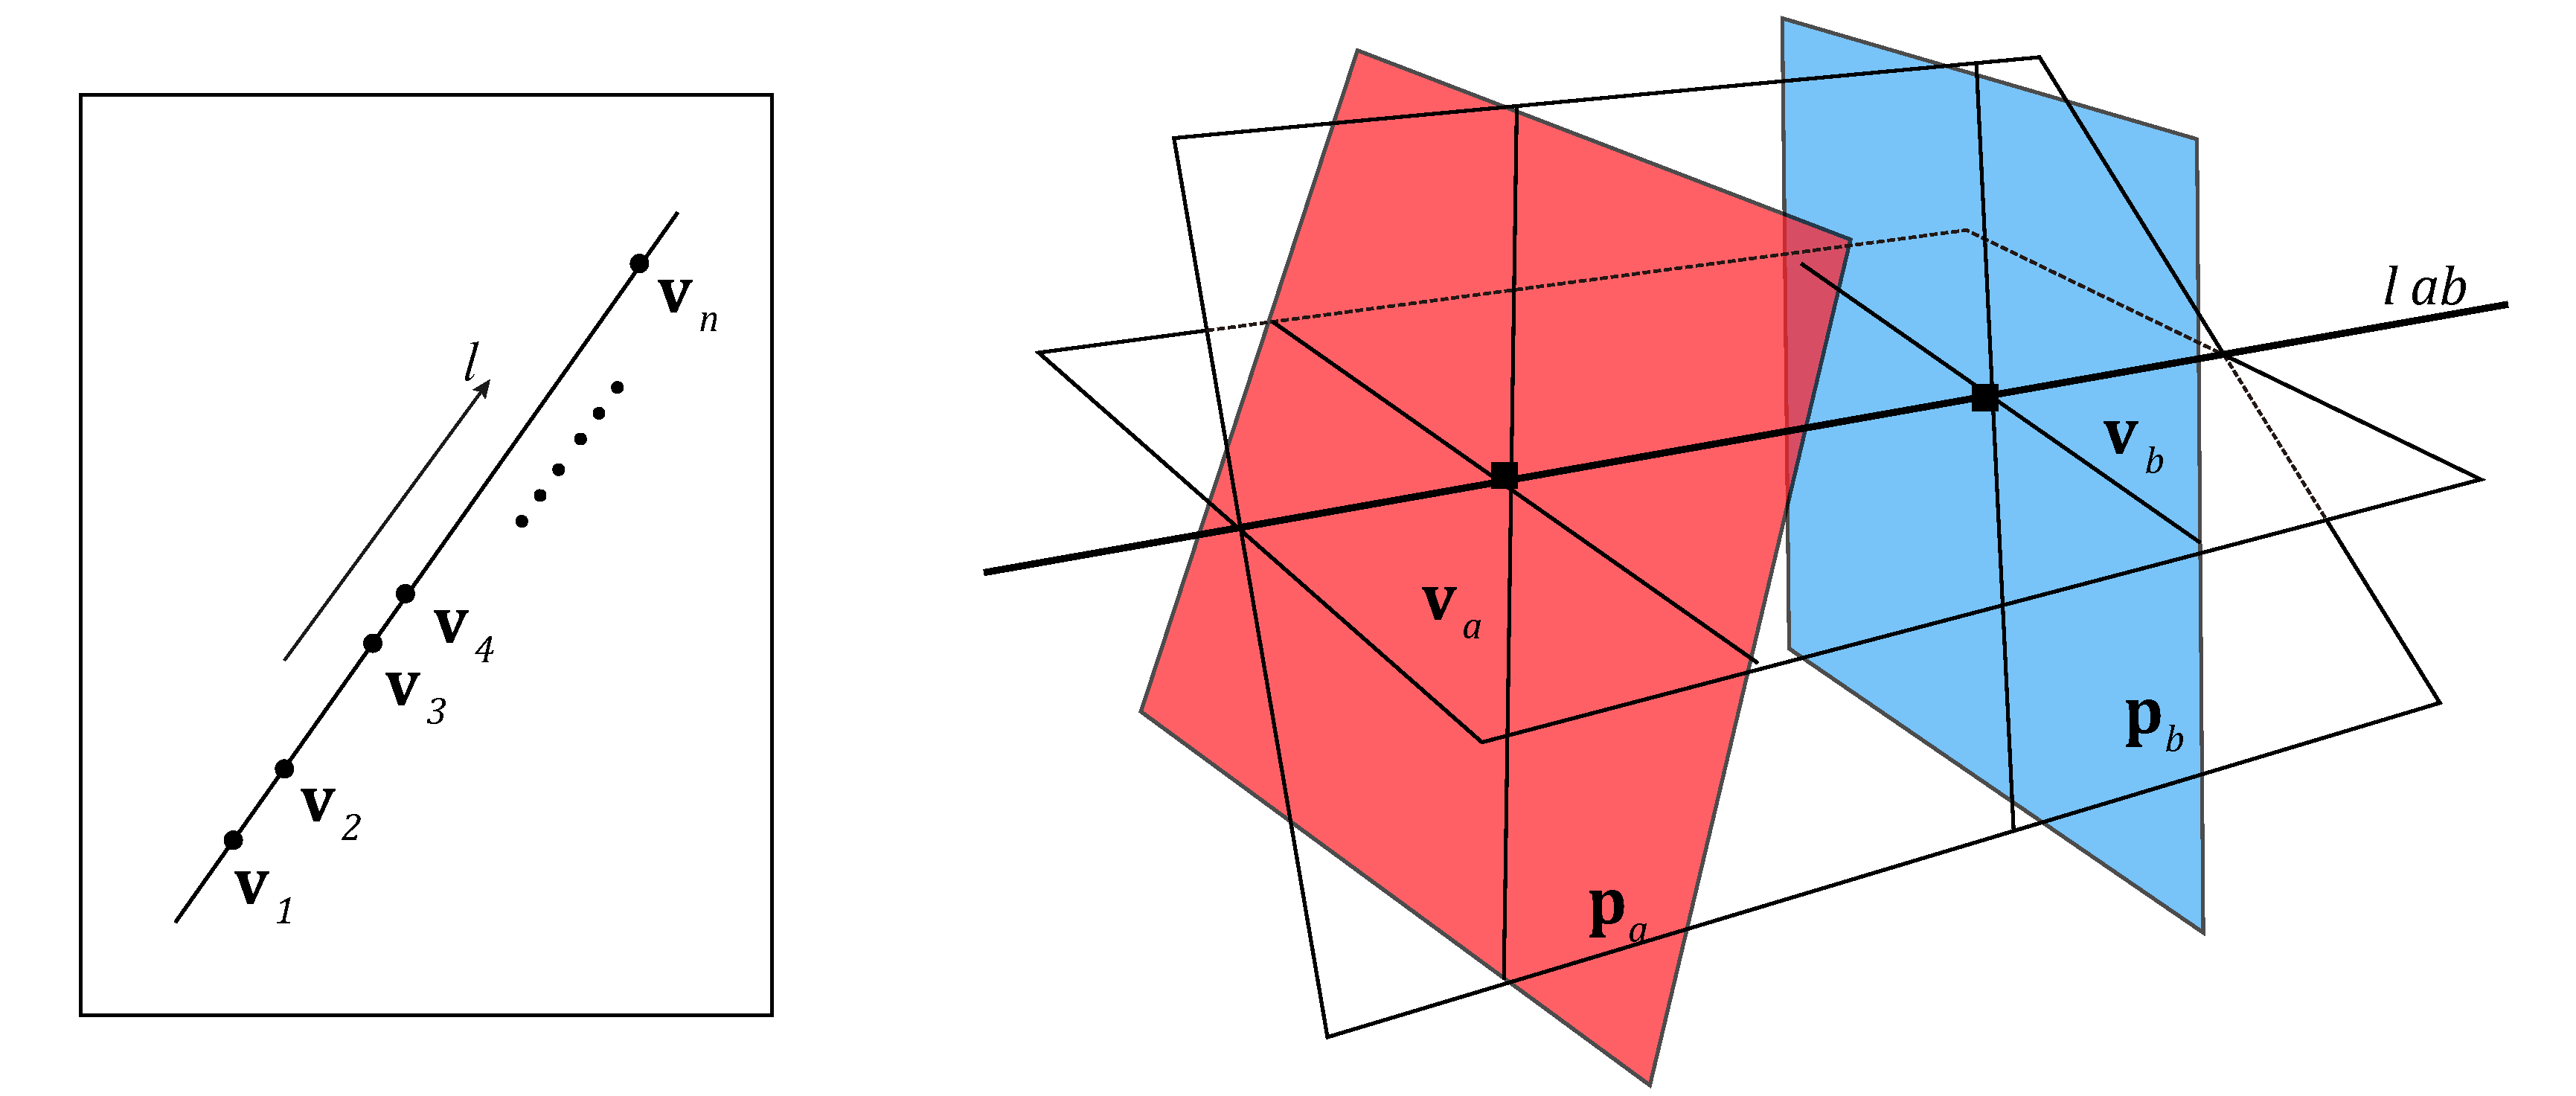
\includegraphics[width=3.5in]{twopointoneline}\\
  \caption{Geometric configuration of the linear ordering of points. Points $\bm{v}_a$ and $\bm{v}_b$ are both on line $\bm{l}_{ab}$. We convert this problem into the plane ordering of $\bm{p}_a$ and $\bm{p}_b$ along $\bm{l}_{ab}$.}\label{fig:twopointoneline}
\end{figure}

\noindent Given a line $\bm{l}_{ab}$ with two points on it, $\bm{v}_a\colon(\bm{p}_a^0\cap\bm{p}_a^1\cap\bm{p}_a^2)$, and $\bm{v}_b\colon(\bm{p}_b^0\cap\bm{p}_b^1\cap\bm{p}_b^2)$, we need to determine the linear order of the two points along $\bm{l}_{ab}$ (see Fig. \ref{fig:twopointoneline}).
To solve this problem, we choose one plane that is not parallel with $\bm{l}_{ab}$ from the P-rep of each point, then convert this problem into one of determining the linear order of planes, which can be solved using the method of Banerjee et al. \cite{banerjee1996topologically}. The chosen planes should have the same orientation with respect to $\bm{l}_{ab}$ (the dot product between the plane normal and $\bm{l}_{ab}$ must be positive), and unqualified planes need to be flipped.


\begin{wrapfigure}{r}[0in]{0in}
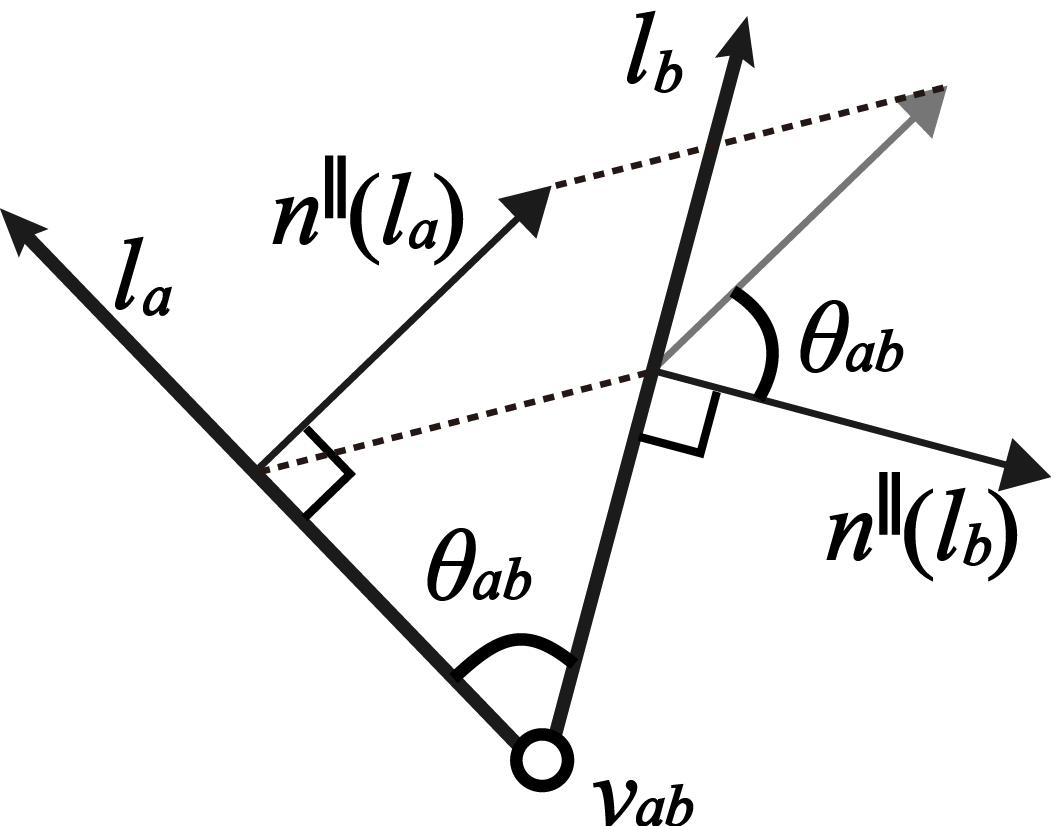
\includegraphics[width=1.5 in]{boolean-02}
\end{wrapfigure}
\vspace{0.5em}
\noindent \textbf{Circular ordering of lines}~~~~

\noindent During face tessellation, we need to know which intersections are neighbors (see Fig. \ref{fig:circularorder}). This requires circular ordering of directed lines around a vertex. The Lines can be sorted in a divide-and-conquer way, based on the relative order of each pair of lines. Thus, this problem is converted to one where, given two lines $\bm{l}_a$ and $\bm{l}_b$ in a plane $\bm{p}_0$, circular order of the two lines needs to be computed.
We can compute the order by the sign of $\sin{\theta_{ab}}$, where $\theta_{ab}\in(-\pi,\pi)$ is the angle from $\bm{l}_a$ to $\bm{l}_b$ in the top-view of $\bm{p}_0$.

We know the sign of $\sin{\theta_{ab}}$ is the same as the sign of $\bm{n}(\bm{p}_0) \cdot (\bm{l}_a\times\bm{l}_b)$. However, directly computing this equation requires extra precision to explicitly compute $\bm{l}_a$ and $\bm{l}_b$. Fortunately, we found a efficient solution which only needs to compute the sign of a 3$\times$3 determinants, whose elements are all floating-point numbers.

\begin{theorem}
  \label{theorem1}
  Given two directed lines $\bm{l}_a\colon(\bm{p}_0\cap\bm{p}_a)$ and $\bm{l}_b\colon(\bm{p}_0\cap\bm{p}_b)$ within plane $\bm{p}_0$, the following relation always stands:
  \begin{equation}
    sign(\sin{\theta_{ab}})=  sign(\bm{n}(\bm{p}_0)\cdot(\bm{n}(\bm{p}_a) \times \bm{n}(\bm{p}_b)))
  \end{equation}
\end{theorem}

\begin{proof}
 First, $\bm{n}(\bm{p}_a)$ and $\bm{n}(\bm{p}_b)$ are orthogonally decomposed along $\bm{n}(\bm{p}_0)$:
 \begin{equation}
 \begin{split}
   &\bm{n}(\bm{p}_a)= \bm{n}^\parallel(\bm{p}_a) + \bm{n}^\perp(\bm{p}_a)\\
   &\bm{n}(\bm{p}_b)= \bm{n}^\parallel(\bm{p}_b) + \bm{n}^\perp(\bm{p}_b),
 \end{split}
 \end{equation}
 where the superscript $\parallel$ refers to the component parallel with $\bm{p}_0$ and $\perp$ means the component orthogonal to $\bm{p}_0$. Since $\bm{n}(\bm{p}_0)$ is orthogonal with $\bm{p}_0$, we get:
 \begin{equation}
   \label{eq:circ1}
   \bm{n}(\bm{p}_0) \cdot (\bm{n}(\bm{p}_a) \times \bm{n}(\bm{p}_b)) = \bm{n}(\bm{p}_0) \cdot (\bm{n}^\parallel(\bm{p}_a) \times \bm{n}^\parallel(\bm{p}_b)).
 \end{equation}
 On the other hand, the angle between $\bm{n}^\parallel(\bm{p}_a)$ and $\bm{n}^\parallel(\bm{p}_b)$ is exactly $\theta_{ab}$. Therefore,
 \begin{equation}
   \label{eq:circ2}
   sign(\sin{\theta_{ab}})=  sign(\bm{n}(\bm{p}_0) \cdot (\bm{n}^\parallel(\bm{p}_a) \times \bm{n}^\parallel(\bm{p}_b))).
 \end{equation}
 By (\ref{eq:circ1}) and (\ref{eq:circ2}), the theorem is proved.
\end{proof}

\begin{figure}[t]
\centering
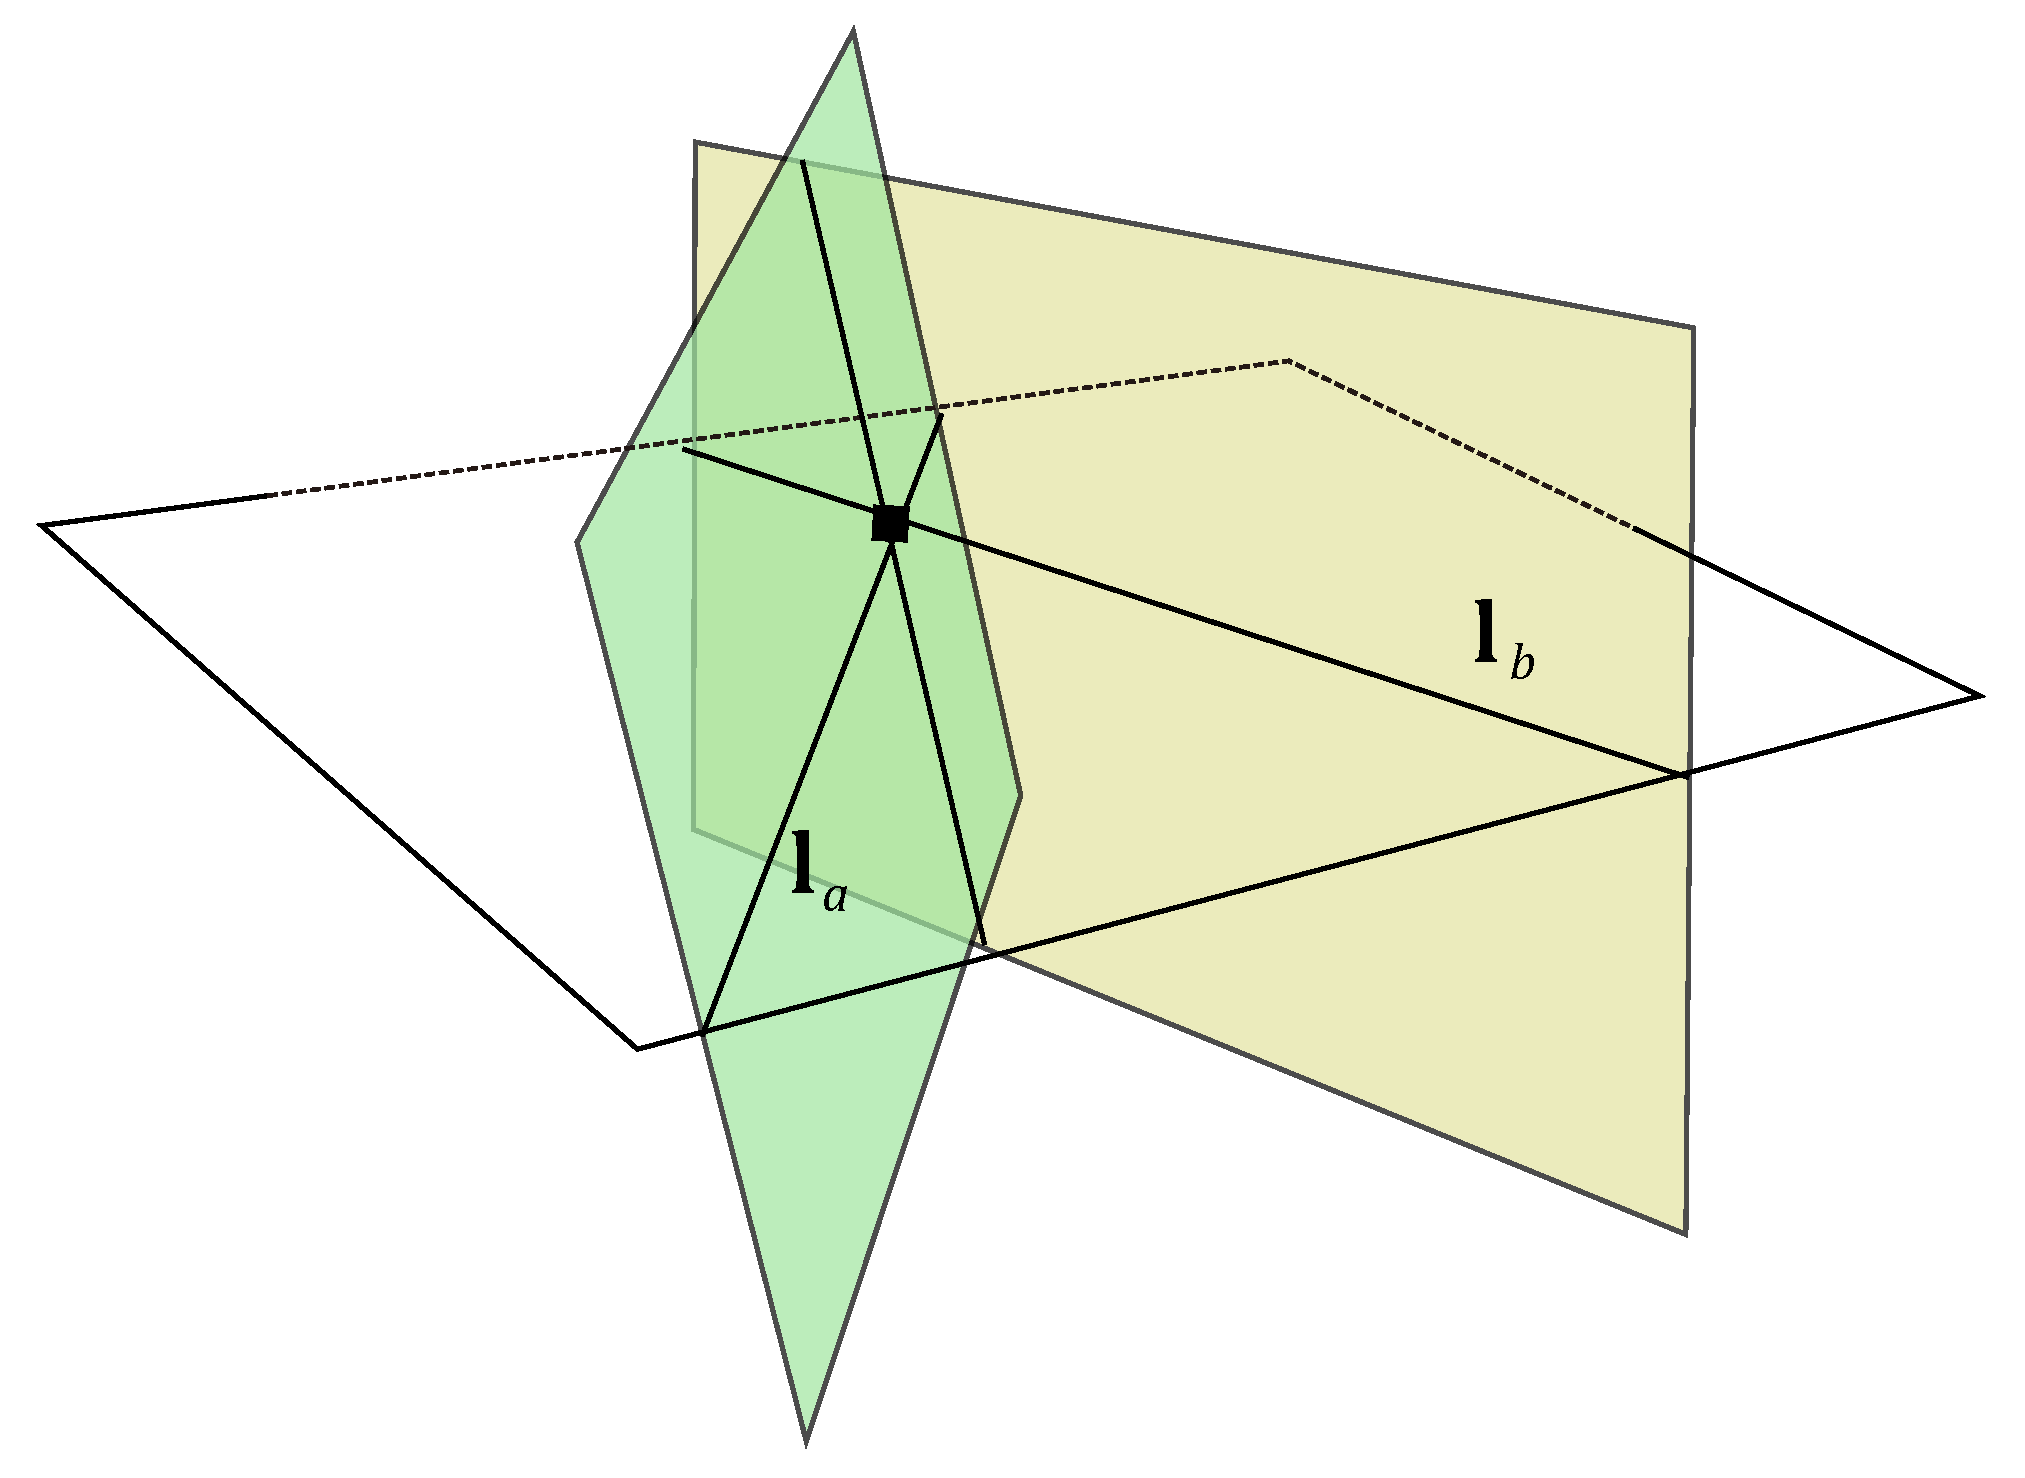
\includegraphics[width=3.5in]{circularorder}
\caption{Geometric configuration of the circular ordering of lines. $\bm{l}_a\colon(\bm{p}_0 \cap \bm{p}_a)$ and $\bm{l}_b\colon(\bm{p}_0 \cap \bm{p}_b)$ are within plane $\bm{p}_0$.}
%Geometric configuration of the circular ordering of lines. la:
\label{fig:circularorder}
\end{figure}

\subsection{Method Overview}


%There are three steps to our method. The first step is to compute the intersections between each triangle face pair. In the second step, the input meshes are tessellated into intersection-free meshes according to these intersections. Lastly, each face is classified and the final mesh is generated.

Before going into details, we give an overview of our method. While the framework is similar to a V-rep based boolean method, we address the major differences in each stage and briefly explain why these differences are necessary.

\subsubsection{Intersection computation}

In this step, we compute the intersections between pairs of triangles. The triangle-triangle intersection algorithm is largely based on M\"{o}llers algorithm \cite{moller1997fast}. However, the conventional V-rep based implementation of M\"{o}ller's algorithm introduces numerical errors. Our P-rep based intersection algorithm implicitly represents intersections using planes to avoid errors. In addition, we carefully deal with degenerate cases, including point intersections, edge intersections, and coplanar intersections. Furthermore, octree is used to speed up the process. Details are provided in \S\ref{section:isect}.

\subsubsection{Deferred tessellation}

%Once all intersections between triangles are detected, we need to tessellate the input meshes and construct the intersection-free meshes. In many methods like \cite{ogayar2015deferred}, constraint Delaunay triangulation (CDT) is applied to perform tessellation. However, for a CSG with more than two meshes, intersections may overlap or intersect with each other, and cannot be used for constraints of CDT directly. In addition, as our intersections are represented by planes, implementation of CDT are complex and inefficient, as most CDT algorithms (e.g. \cite{chew1989constrained}, \cite{de1992line}) is not designed to handle planes and requires explicit coordinates. Therefore, we first perform intersection refinement to resolve intersecting intersections. After that, we construct a graph-like structure suitable for P-rep intersections, called \emph{tess-graph}, to guide the exact tessellation of each face. After all faces are tessellated, we get our intersection-free meshes. Details are shown in \S\ref{sec:tessellation}.

Once all of the intersections between triangles are determined, input meshes are subdivided, so that all intersections occurs on edges and vertices. In many existing methods (e.g., \cite{ogayar2015deferred,zhou2016mesh}), 2D constrained Delaunay triangulation (CDT) \cite{chew1989constrained}\cite{de1992line} is used to implement this stage. In our method, intersections are represented by planes. Therefore, projection is not allowed and the 2D CDT has to be mapped to an equivalent 3D problem. However, a 2D CDT needs to construct edges between arbitrary pair of vertices, whose equivalent 3D operation is to construct new planes which contains arbitrary two vertices. The newly constructed planes require extra precision to represent, and computations with them are slow.

Therefore, we choose to tessellate in a more conservative way that do not add any new edges. As a consequence, the subdivided faces are no more triangles. We first perform intersection refinement to resolve intersections between intersections to make them \emph{regularized}. We then construct a graph-like structure, called a \emph{tess-graph}, to guide the exact tessellation of each face. Details are given in \S\ref{sec:tessellation}.

\subsubsection{Face classification}

The purpose of this step is to collect faces that pass the CSG expression from the tessellated meshes to generate the final mesh. However, literally computing the inclusion label vector of each face is unacceptably slow for large CSGs. We utilize the connectivity information to propagate inclusion labels in a flood-filling manner. The seed labels used for flood-filling have to be computed beforehand. Typically, a seed face label is deduced by the label of point on that face. However, the point label can be incorrectly computed without exact arithmetic. We exactly computed face label by a local BSP constructed according to the faces of neighborhoods. Our algorithm does not requires exact arithmetic. Also, the constructed BSP is typically small, which resulting in good performance. Details are given in \S\ref{sec:classification}.


\begin{figure}[t]
\centering
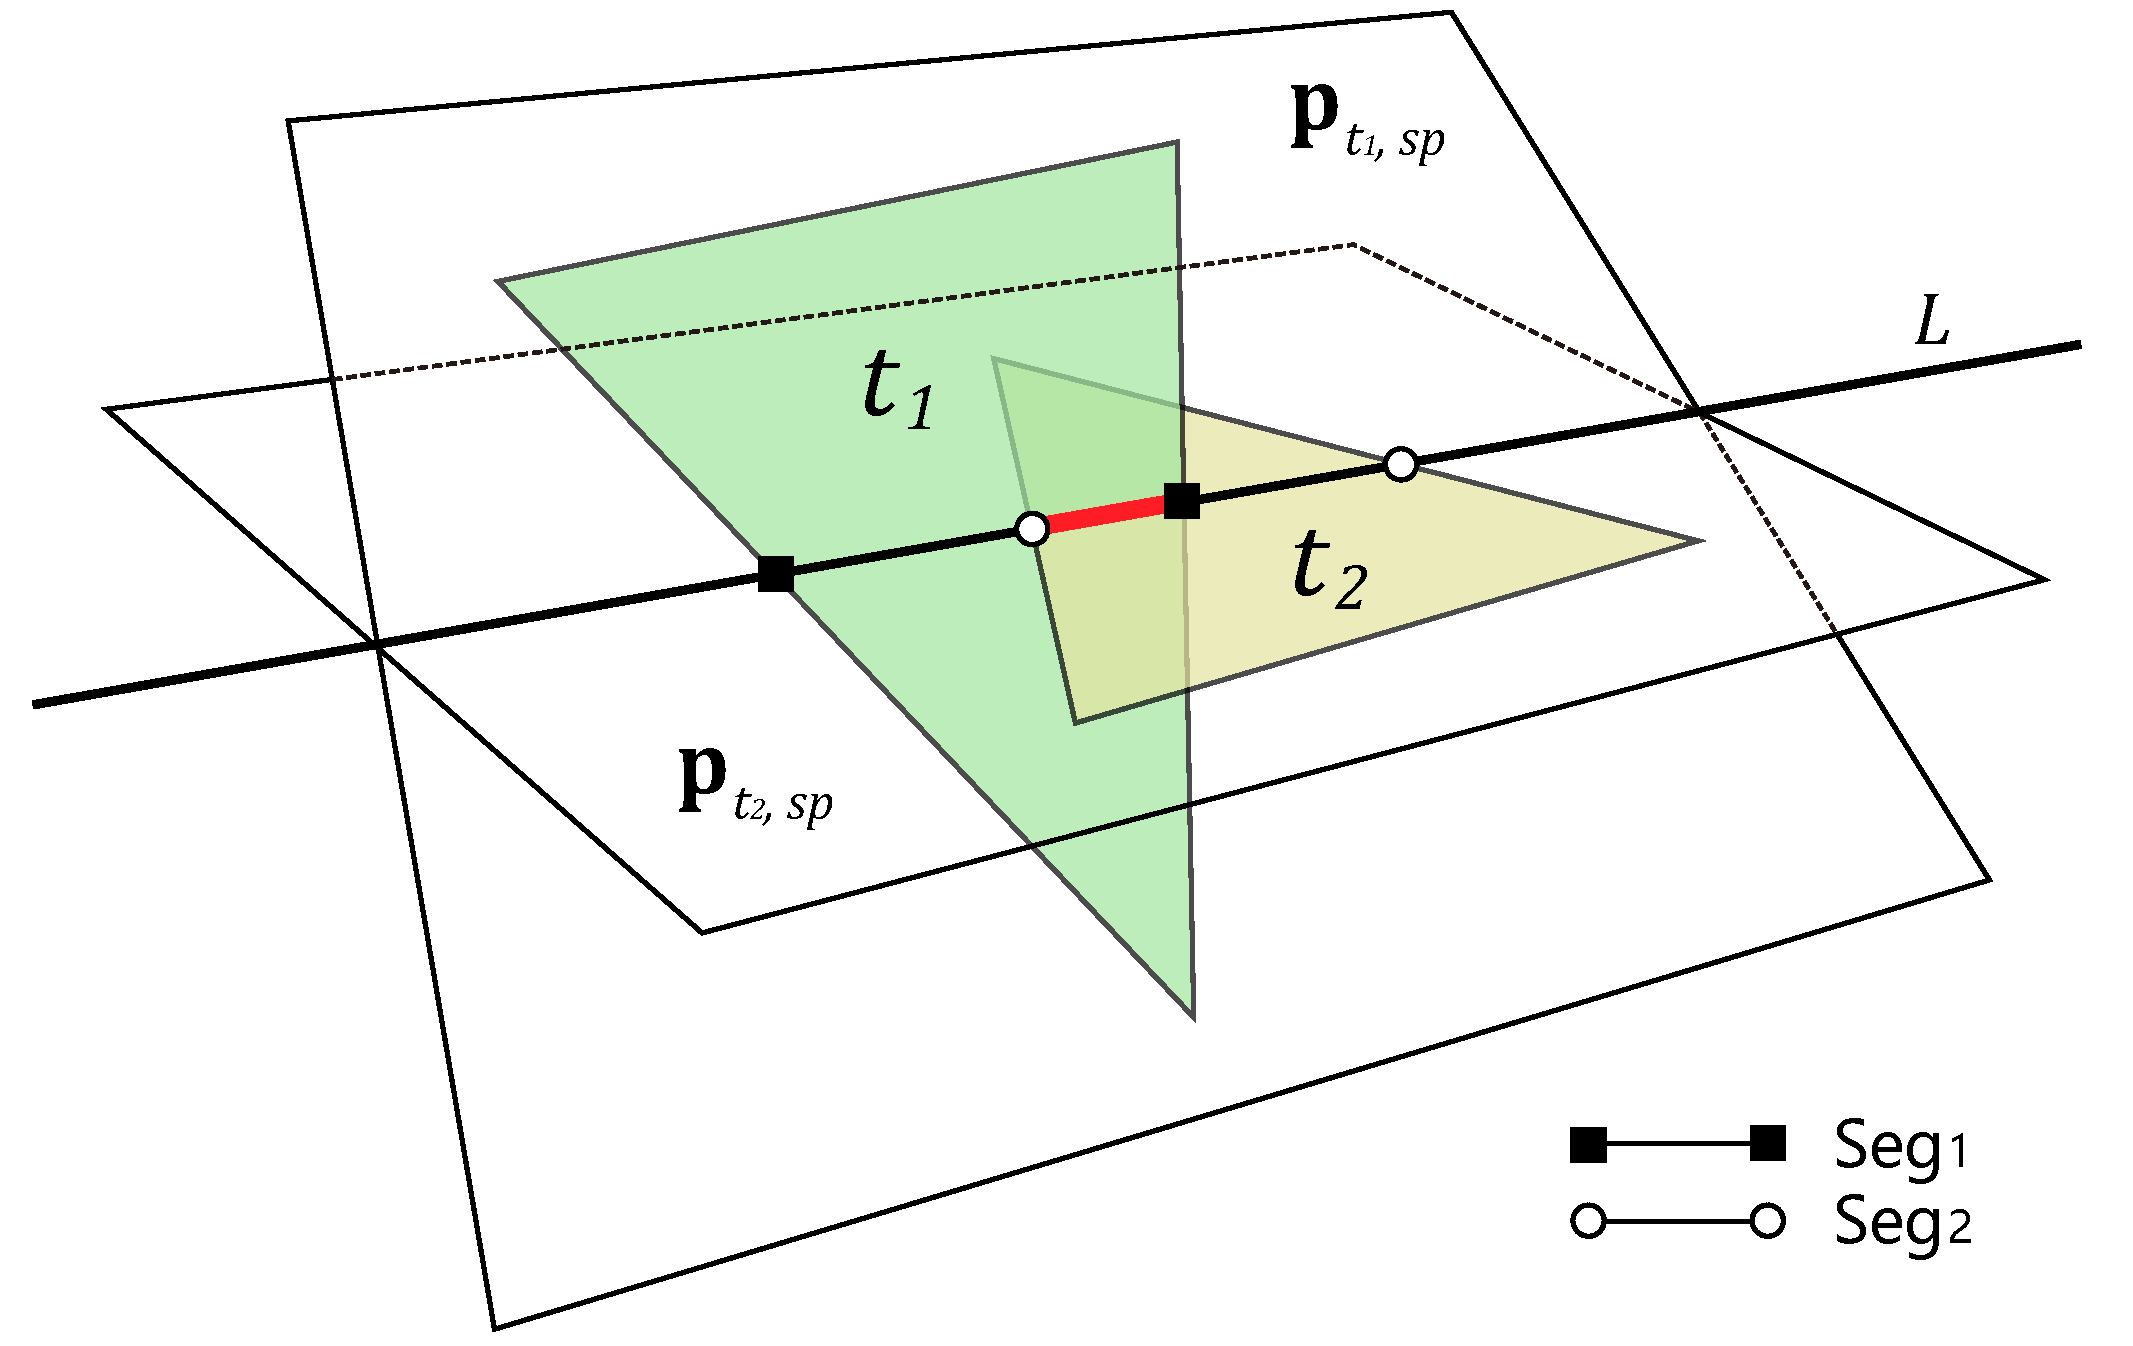
\includegraphics[width=2.5in]{projection}
\caption{$Seg_1$ is the intersection between $\bm{p}_{t_2, sp}$ and $t_1$. $Seg_2$ is the intersection between $\bm{p}_{t_1, sp}$ and $t_2$. The intersection between $t_1$ and $t_2$ (yellow line segment) is the overlap of $Seg_1$ and $Seg_2$.}
%Seg1 is the intersection between pt2,sp and t1. Seg2 is the intersection between pt1,sp and t2. The intersection between t1 and t2 (yellow line segment) is the overlap of Seg1 and Seg2.
\label{fig_projection}
\end{figure}

\section{Intersection Computation}

\label{section:isect}
%In this step, intersections between faces are computed through triangle-triangle intersection test. We adopt M\"{o}ller's algorithm \cite{moller1997fast} on account of its efficiency and simplicity. However, a naive implementation of M\"{o}ller's algorithm can introduce numerical errors and may fail to produce correct results. Therefore, we integrate plane-based geometry to make it exact. In the following, we first introduce our space division strategy to reduce the number of intersection test. Then we make a quick review of M\"{o}ller's algorithm, and discuss the way to embed plane-based geometry. After that, we discuss how to deal with degenerate cases.

In this step, the intersections between faces are determined by a triangle-triangle intersection test. We use  M\"{o}ller's algorithm \cite{moller1997fast} because of its efficiency and simplicity. To ensure exact intersection computation, we integrate P-rep based geometry into the algorithm. In the following, we first introduce our space division strategy to reduce the number of intersection tests. Then introduce our P-rep based intersection algorithm. Lastly, we discuss how to deal with degenerate cases.

\subsection{Space Division}
\begin{wrapfigure}{r}[0in]{0in}
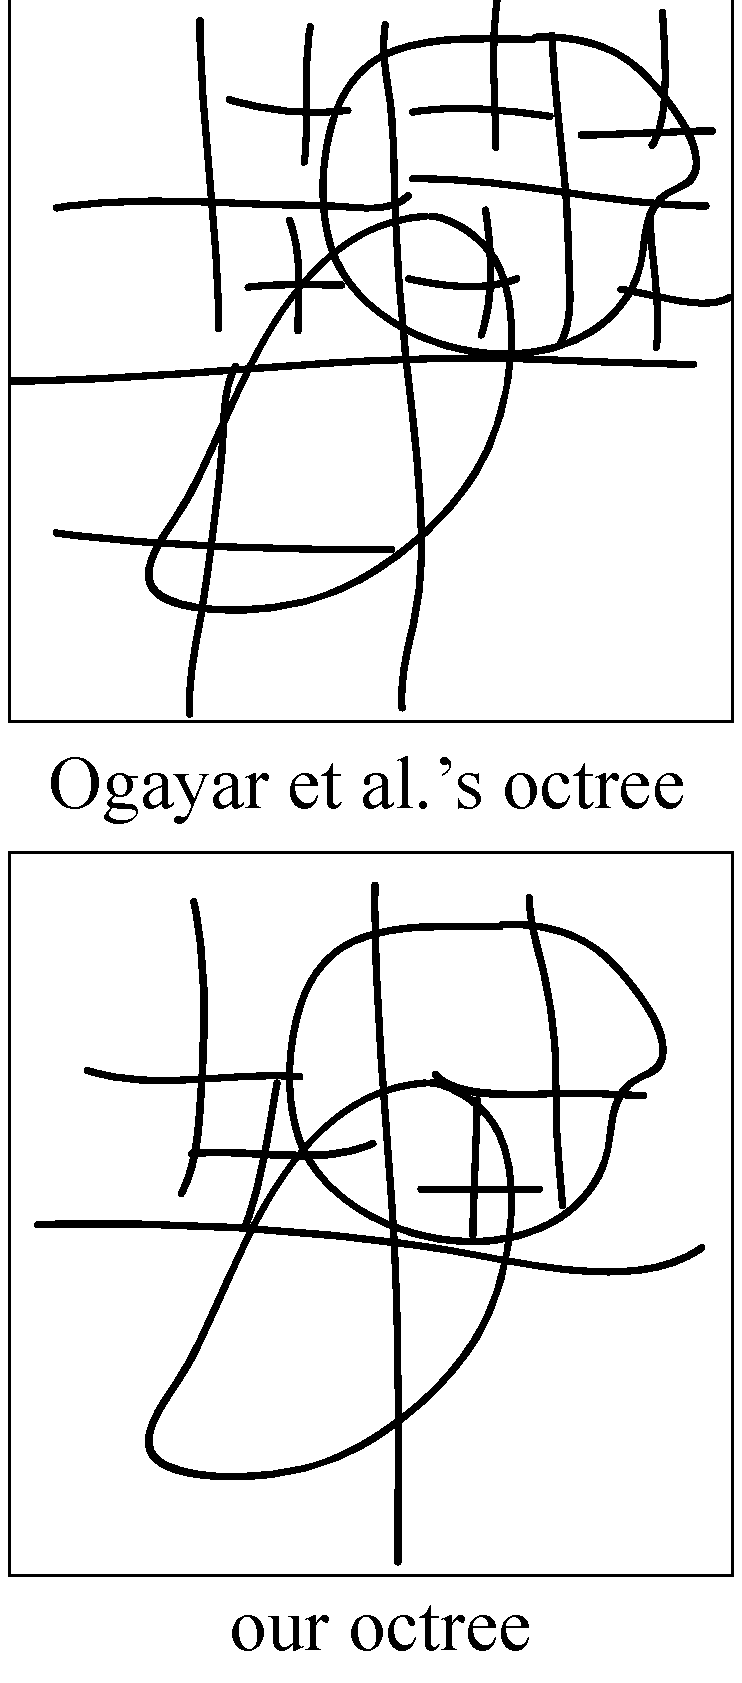
\includegraphics[width=1.2in]{octreediff}
\end{wrapfigure}


%As intersection detection is performed between each pair of faces, localization is necessary for large CSGs to reduce the number of testing pairs. We use the adaptive octree for this purpose. Our implementation is akin to the implementation in Ogayar et al.'s method \cite{ogayar2015deferred}. Intersection between triangle faces and octree nodes are efficiently detected using the separating axis theorem \cite{gottschalk1996obbtree}. Octree leaves are classified into two types: if all faces that intersect a leaf belong to the same mesh, we call it a \emph{normal cell}. Otherwise, it is a \emph{critical cell}, within which the following intersection computation is performed.

As intersection detection is performed between each pair of faces, space division is necessary to reduce the number of pairs to be tested. We use an adaptive octree for this purpose. Our implementation is akin to the implementation of Ogayar et al. \cite{ogayar2015deferred}. The intersections between triangle faces and octree nodes are efficiently detected using the separating axis theorem \cite{gottschalk1996obbtree}. Octree leaves are classified into two types. If all faces that intersect a leaf belong to the same mesh, we regard it as a \emph{normal cell}. Otherwise, it is regarded as a \emph{critical cell}, within which the following intersection computation is performed.

%The difference between our octree and Ogayar et al.'s is that we do not subdivide any normal cell no matter how many faces it contains. This is because subdividing normal cells benefits only the point-in-polyhedron test \cite{frisken2002simple}, which seldom uses in our method. This simplification can save much computing time, especially when intersections between primitives are not complex and located in small regions.

The difference between our octree and that of Ogayar et al. is that we do not subdivide any normal cell, no matter how many faces it contains. Subdividing normal cells is only beneficial for the point-in-polyhedron test \cite{frisken2002simple}, which is seldom used in our method. This simplification saves significant computing time, especially when intersections between primitives are simple, and located in small regions.

\subsection{Plane-Based Intersection Test}

We first make a quick review of M\"{o}ller's V-rep based algorithm. Then we introduce our implicit representations of intersections using planes. After that, we discuss how to implement  M\"{o}ller's algorithm using P-rep based geometry.

\subsubsection{Review of M\"{o}ller's algorithm}



M\"{o}ller's algorithm computes the intersection between two triangles $t_1$ and $t_2$ in three steps as shown in Fig. \ref{fig_projection}:
\begin{itemize}[leftmargin=0.45cm]
\item[1)] An early rejection is performed by testing whether $t_1$ intersects $\bm{p}_{t_2, sp}$, the supporting plane of $t_2$. The same test is also carried out between $t_2$ and $\bm{p}_{t_1, sp}$.
\item[2)]The intersection between $t_1$ and $\bm{p}_{t_2, sp}$, denoted as $Seg_1$, and the intersection between $t_2$ and $\bm{p}_{t_1, sp}$, denoted as $Seg_2$, are computed separately.
 \item[3)]The intersection between $t_1$ and $t_2$ is determined by computing the overlap between $Seg_1$ and $Seg_2$ .
\end{itemize}



The non-robustness of this algorithm stems from computing the coordinates of the intersection vertices (the end points of $Seg_1$ and $Seg_2$). Although implementation of this algorithm with arbitrary precision arithmetic produces exact coordinates, it is too costly for boolean operations with large CSGs. We use plane-based geometry to solve this problem, by implicitly representing intersections with planes.

\subsubsection{Plane-based intersection representation}
\label{sec:ir}

In our method, the intersection with triangle $t$ is stored as $\bm{\mathcal{I}}\colon\{T, \bm{P}_{ext}, \bm{P}_0, \bm{P}_1, \mathcal{N}\}$. This is the plane-based intersection representation (PBI-rep,  see Fig. \ref{fig:pbi}). The first component, $T$, indicates which triangle $\bm{\mathcal{I}}$ lies on.
$\bm{P}_{ext}$ indicates the plane that $\bm{\mathcal{I}}$ lies on. Note that $T$ is not in $\bm{P}_{ext}$. The first two components indicate that  $\bm{\mathcal{I}}$ lies on the line $T \cap \bm{P}_{ext}$.
The two end points of $\bm{\mathcal{I}}$ are $T \cap \bm{P}_{ext}\cap\bm{P}_0$ and $T \cap \bm{P}_{ext}\cap\bm{P}_1$.
The last component, $\mathcal{N}$, represents the neighborhood faces of $\bm{\mathcal{I}}$. $\mathcal{N}$ can be a single face, or a set faces from different input primitives.

\begin{figure}[t]
\centering
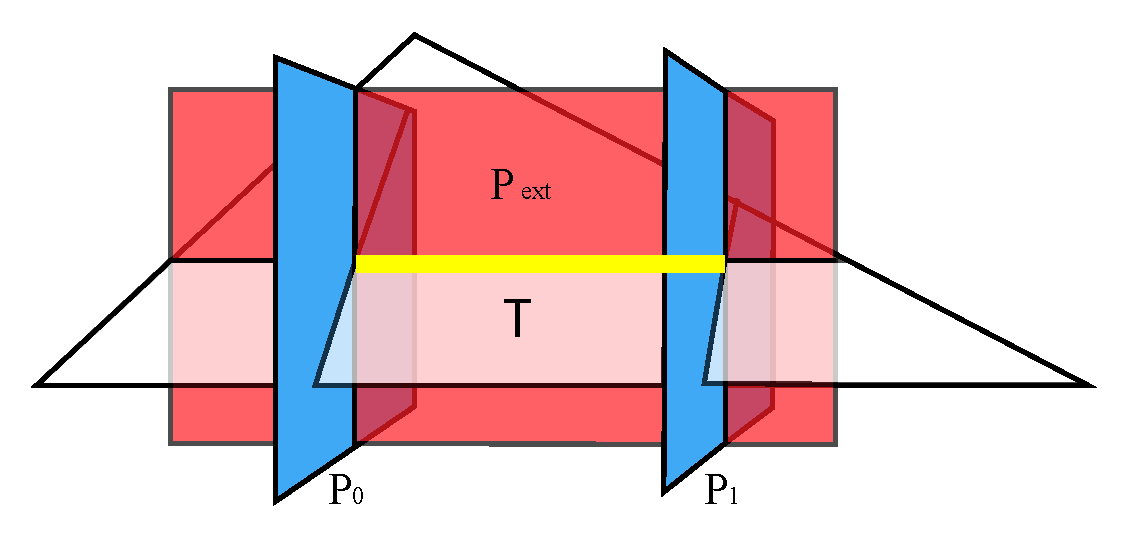
\includegraphics[width=3in]{pbirep2}
\caption{The geometry of planes in a PBI-rep. The yellow line segment is the intersection represented by $\bm{\mathcal{I}}$.}
\label{fig:pbi}
\end{figure}

For example, two triangle faces, $t_1$ and $t_2$, originating from meshes $M_i$ and $M_j$, respectively, intersect. Two intersections are generated, ${\bm{\mathcal{I}}}_{12}$ on $t_1$ and ${\bm{\mathcal{I}}}_{21}$ on $t_2$.
For ${\bm{\mathcal{I}}}_{12}$, $T = t_1$ and $\bm{P}_{ext}=\bm{p}_{t_2, sp}$. $\bm{P}_0$ and $\bm{P}_1$ are boundary planes of $t_2$, which will be discussed later.
The last component $\mathcal{N}=t_2$ in general situation. Sometimes, ${\bm{\mathcal{I}}}_{12}$ may lie on the edge of $t_2$ (see Fig. \ref{fig:twin}). This is called \emph{edge intersection}. In this situation, the $\mathcal{N}$ is the set of all faces from $M_j$ adjacent to that edge. Edge intersection is discussed in \S\ref{sec:degenerate}.


\subsubsection{Plane-based implementation}

\label{sec:embed}
\begin{figure}[t]
\centering
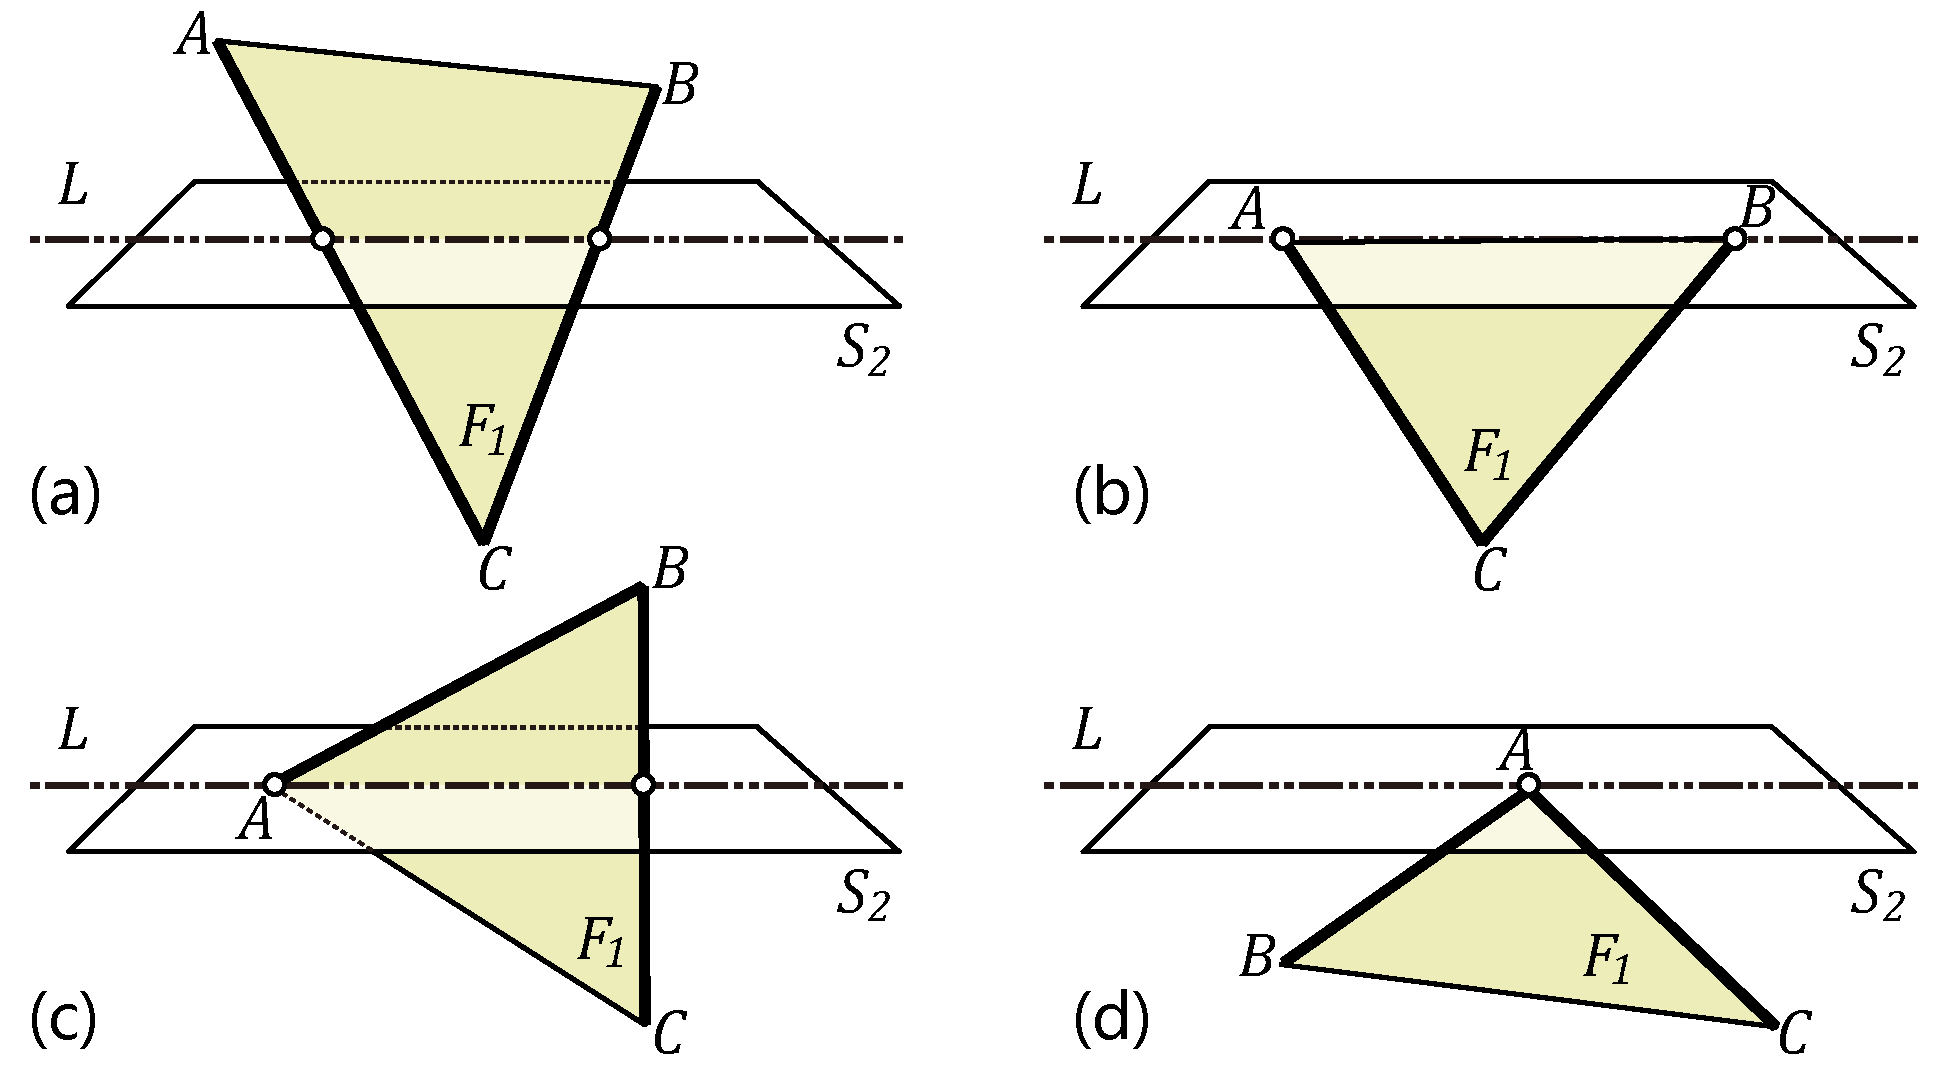
\includegraphics[width=3.5in]{sign}
\caption{We denote the signed distance from point $v_i$ to plane $\bm{p}_{t_2, sp}$ as $d_i$. The four conditions of intersection between $t_1$ and $\bm{p}_{t_2, sp}$ are:
(a) $d_0\cdot d_2<0$, $d_1\cdot d_2<0$;
(b) $d_0=0$, $d_1=0$, $d_2\neq 0$;
(c) $d_0=0$, $d_1\cdot d_2<0$;
(d) $d_0=0$, $d_1\cdot d_2>0$. End points of $Seg_1$ are the intersections between $\bm{p}_{t_2, sp}$ and the related edges of $t_1$ (bold red lines).}
\label{fig:isect}
\end{figure}

To implement M\"{o}ller's algorithm by plane-based geometry, we first convert each triangle to its P-reps: a supporting plane $\bm{p}_{t, sp}$  surrounded by three bounding planes $\{\bm{p}_{t, b}^i|\ i = 0,1,2\}$. The substrates of the intersection algorithms are point-plane orientation \cite{bernstein2009fast} and linear order of points (\S\ref{sec:substrates}), both of which can be implemented by plane-based geometry.

In the first step, the computation of signed distances involves only the vertices coordinates and the supporting planes of triangles. Therefore, if the early rejections occur, the bounding planes are not needed at all. In addition, according to the conversion method of Campen et al.\cite{campen2010exact}, the supporting plane is represented by four double precision floating point numbers. The precision of first three parameter $L_a$ and the precision of the last parameter $L_d$ hold the relation $L_d = L_a + L + 1$, where $L$ is the precision of coordinates of input vertices. This means we can compute the signed distance exactly within double-precision. With these two facts, our early rejection is as fast as the vertex-based implementation.

If $t_1$ and $t_2$ are not coplanar, $Seg_1$ and $Seg_2$ are computed. The end points are intersections between the supporting plane of one triangle and an edge of the other triangle. By computing the bounding planes, the end points can be implicitly represented by plane triples, $\bm{p}_{t_2, sp} \cap \bm{p}_{t_1, sp} \cap \bm{p}^i_{t_1, b}$, where $\bm{p}^i_{t_1, b}$ is the bounding plane of the related edge.
Fig. \ref{fig:isect} shows all of the possible intersection conditions between $t_1$ and $\bm{p}_{t_2, sp}$. The coplanar situation is discussed in \S \ref{sec:degenerate}.

To avoid repetitive vertices in the final result, we perform vertex repetition elimination in this step. Because P-reps are used, the coincidence tests of the vertices are exact.



\subsection{Handling Degenerate Case }
\label{sec:degenerate}

%While two triangles, if intersecting, intersect on a line segment in most situations, they can also intersect on a point or a convex area (coplanar case). Even if the intersection is a line segment, the intersection can be on triangle edges. These degenerate situations prevent us from performing robust boolean operations. In this section, we offer simple but effective way to deal with all these degenerations, which conceals the complexity of intersections and simplifies later processing.

In most situations, two intersecting triangles intersect on a line segment. However, they can also intersect on a point or a convex area (coplanar case). Even if the intersection is a line segment, the intersection can be on an edge. These degenerate situations prevent us from performing robust boolean operations. In this section, we demonstrate a simple but effective way of dealing with all of these degenerations, which conceals the complexity of intersections, and simplifies later processing.

%%%The criterion of whether an intersection help tessellation is by its necessity: if the intersection is not presented, whether some faces from the linked halfedge will cross the boundary of primitives. The word 'cross' do not only include the situation that a face is partly outside and partly inside of a primitive, but also can mean that a face is partly inside (outside) and part on the boundary of the primitive.


\subsubsection{Point intersection}
\label{sec:ipoint}
%If two triangles intersect on a single point (e.g., Fig. \ref{fig:isect}d), the intersection cannot be represented using our four-component description since the line segment collapses into a single point. In these cases, we simply add the intersection point into the related triangles to guarantee correct tessellation. No intersection is introduced.

If two triangles intersect at a single point (such as in Fig. \ref{fig:isect}d) then the intersection cannot be represented using our four-component description, because the line segment collapses into a single point. In these cases, we simply add the intersection point into the related triangles, which guarantees correct tessellation. No further intersections are introduced.

\subsubsection{Edge intersection}


%When intersection line segment lies on the edge of face, we call it \emph{edge intersection}. The space near edge intersection is divided by faces around the intersected edge (typically two faces for a manifold edge), instead of just one face. Therefore, the neighborhood of the related intersection is a set of faces instead of a single one. For example, in Fig. \ref{fig:twin}, the neighborhood of the intersection on $t_1$ is $\{t_2, t^*_2\}$.

When an intersecting line segment lies on the edge of a face, we refer to it as \emph{edge intersection}. The space near the edge intersection is divided by the faces around the intersected edge (typically two faces for a manifold edge), instead of by just one face. Therefore, the neighborhood of the corresponding intersection is a set of faces rather than a single face. For example, in Fig. \ref{fig:twin}, the neighborhood of the intersection on $t_1$ is $\{t_2, t^*_2\}$.

%Another thing needs to be noticed is that there will be repetitive detection of edge intersections. For example, in Fig. \ref{fig:twin}a, the same intersection on $t_1$ will be detected twice because $t_1$ intersect both $t_2$ and $t_2^*$ in exactly the same intersection. We solve this duplication together with other interactions among different intersections in \S\ref{sec:tessellation}. We also call such $t_2$ and $t_2^*$ as \emph{companion triangles} in an edge intersection because they share the same edge intersection. This concept will be referred again in the discussion of coplanar cases.

Edge intersections will be repeatedly detected. For example, in Fig. \ref{fig:twin}a, the same intersection on $t_1$ will be detected twice, because $t_1$ intersects both $t_2$ and $t_2^*$ at the same intersection. We solve this duplication, together with similar interactions between different intersections in \S\ref{sec:tessellation}. We regard $t_2$ and $t_2^*$ as \emph{companion triangles}, because they share the same edge intersection. This concept is referred to again in the discussion of coplanar cases.

\begin{figure}[t]
\centering
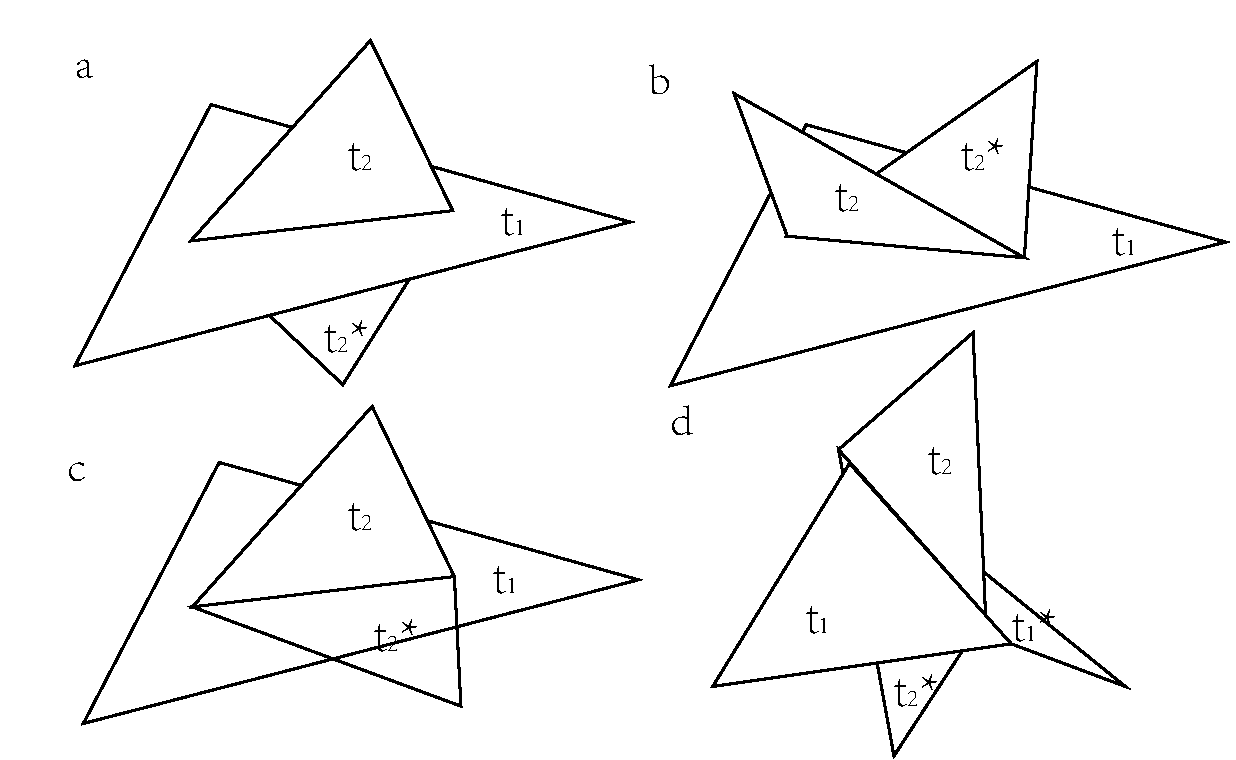
\includegraphics[width=3.5in]{edgeisect}
\caption{Different conditions of edge intersection. Triangle faces $t_1$ and $t_1^*$ are companion faces. Triangle faces $t_2$ and $t_2^*$ are companion faces. a) $t_2$ and $t_2^*$ are on different sides of $t_1$. b) $t_2$ and $t_2^*$ are on the same side of $t_1$. c) $t_2^*$ is coplanar with $t_1$. d) Both $t_1$ and $t_2$ have companion faces: the intersection is an edge intersection for both $t_1$ and $t_2$ (instead of only for $t_2$ is the previous three conditions). }
%Different conditions of edge intersection.
\label{fig:twin}
\end{figure}


\subsubsection{Copalnar}

\begin{figure}[t]
\centering
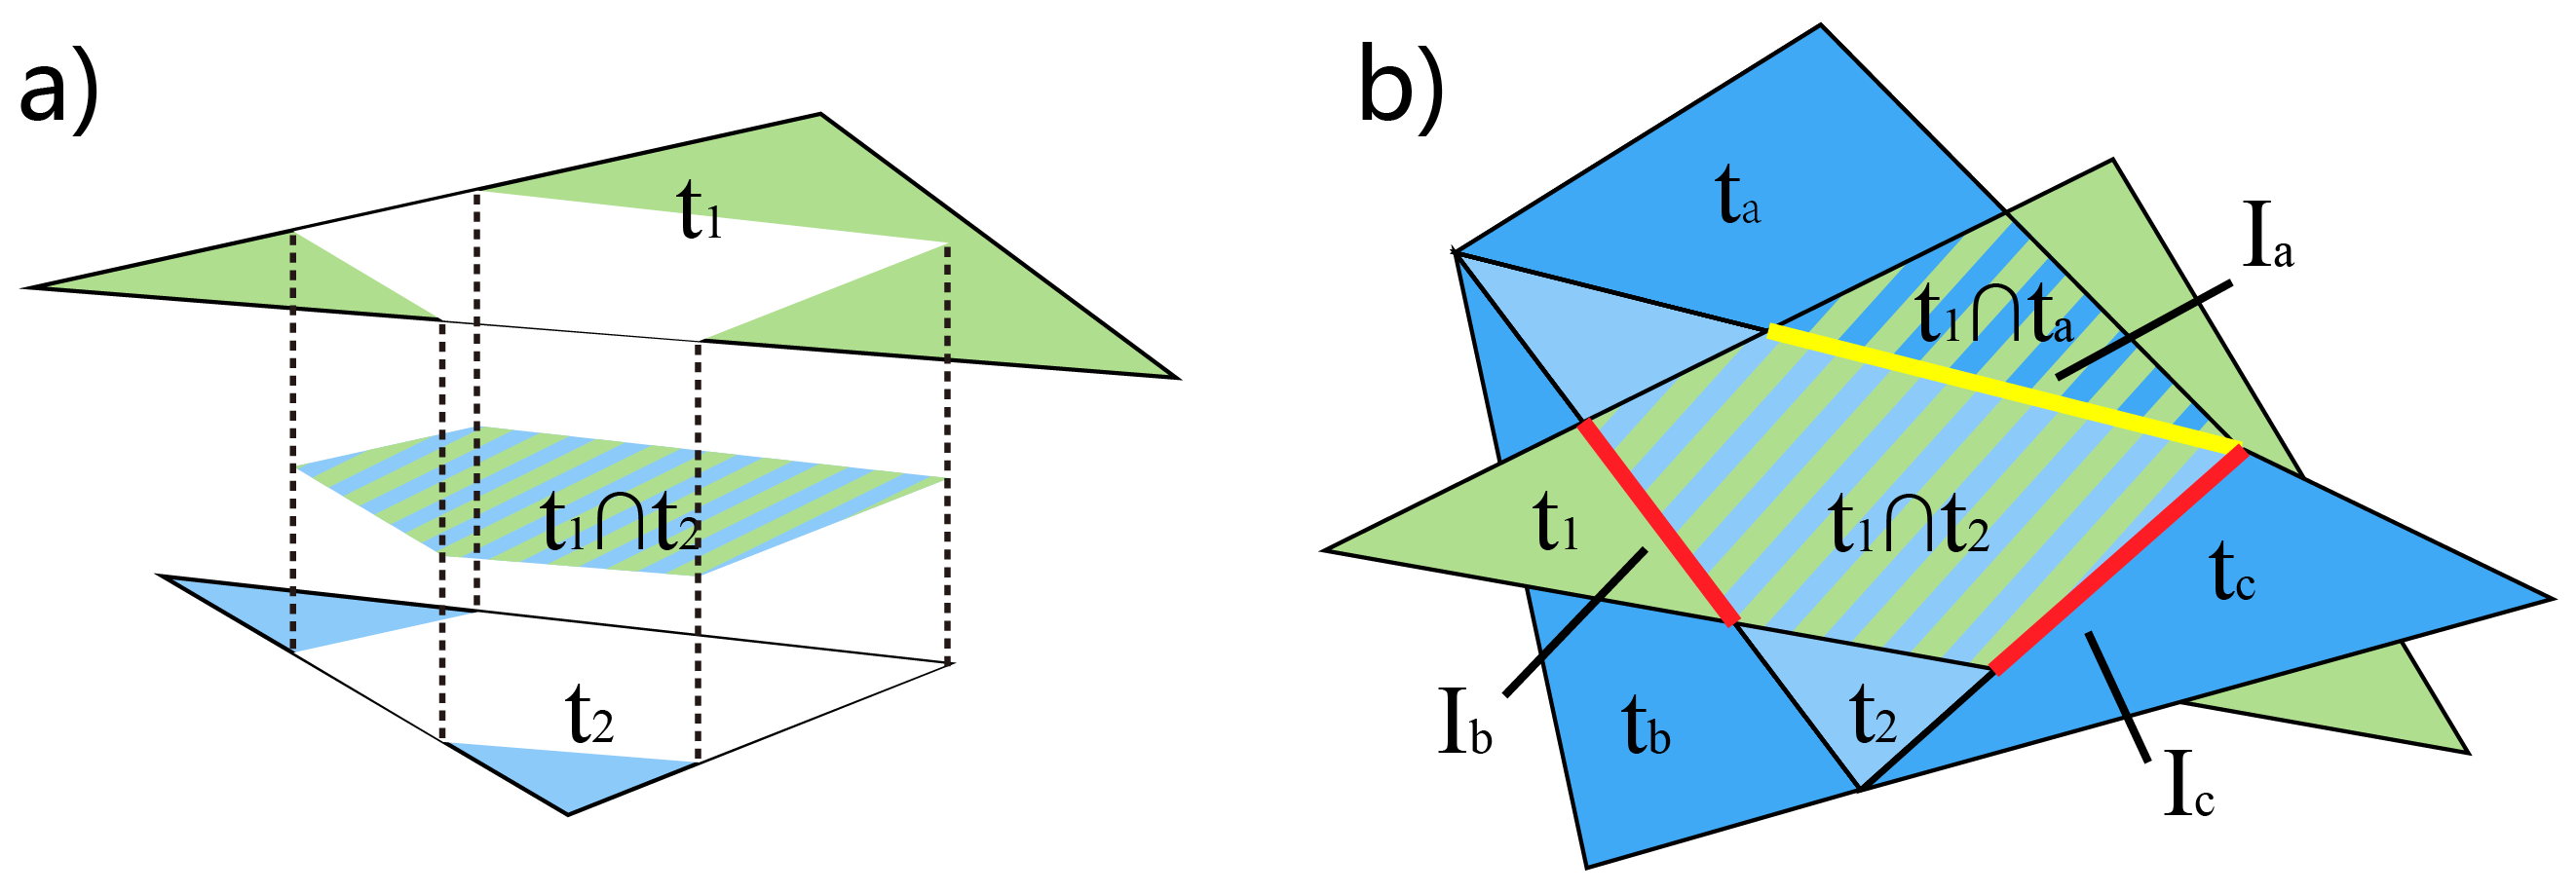
\includegraphics[width=3.5in]{boolean-03}
\caption{a) Coplanar cases; $t_1$ and $t_2$ intersect in 2D, dividing each other into two areas---a convex overlapping area and exclusive areas. b) Possible configurations of the companion faces. The blue triangles originate from the same mesh. For $\mathcal{I}_a$, the companion triangle $t_a$ is coplanar with $t_1$. Therefore, the overlapping areas ($t_1 \cap t_a$ and $t_1 \cap t_2$) do not need to be split by the yellow edge during tessellation, thus $\mathcal{I}_a$ is invalid. For $\mathcal{I}_b$ and $\mathcal{I}_c$, the companion faces are not coplanar, so these intersections can be recorded during an intersection test between $t_1$ and $t_a$ or $t_1$ and $t_b$. There is no need to record the intersection between $t_1$ and $t_2$.}
%Fig. 8. a) Coplanar cases; t1 and t2 intersect in 2D, dividing each other into two areas��a convex overlapping area, and exclusive areas.
\label{fig:coplanar}
\end{figure}

%Consider two triangle faces $t_1\in M_x$ and $t_2 \in M_y$ intersect within a common plane. Both $t_1$ and $t_2$ will divide each other into two areas---a convex overlapping area and exclusive parts (Fig. \ref{fig:coplanar}a). Apparantly, if we tessellate both $t_1$ and $t_2$ according to the boundary of overlapping area, we can guarantee that the tessellated meshes are intersection-free. Many previous methods \cite{feito2013fast,zhou2016mesh} use this method to guarantee topology correctness. However, in our method, we do not test whether $t_1$ and $t_2$ really intersect in 2D once we find they are coplanar. We treat coplanar situations as they do not intersect at all. In this way, we simplify our method, making it more robust and fast, while doing no harm to the topology correctness.

Consider two triangle faces,  $t_1\in M_x$ and $t_2 \in M_y$, which intersect within a common plane. Both $t_1$ and $t_2$ divide each other into two areas��a convex overlapping area and exclusive areas (Fig. \ref{fig:coplanar}a). If we tessellate both $t_1$ and $t_2$ according to the boundary of the overlapping area, we can guarantee that the tessellated meshes are intersection-free. Many previous methods \cite{feito2013fast,zhou2016mesh} use this process to guarantee topological correctness. However, in our method, we do not test whether $t_1$ and $t_2$ really intersect in 2D once we determine that they are coplanar. We treat coplanar situations as if they do not intersect at all. In this way, we simplify our method, making it faster and more robust, while having no effect on the topological correctness.

%We find that each intersection line segment in 2D is part of the edges from input meshes. That means we can view 2D intersection as a special case of edge intersection. The only difference is that there can be up to three edge intersections in one 2D intersection (red and yellow line segments in Fig. \ref{fig:coplanar}b). As we have discussed, edge intersection will be detected twice. That means we can rely on the companion triangle faces to detect intersections.

We find that each intersecting line segment is part of the edges of the input meshes in 2D. That means that we can view 2D intersections as special cases of edge intersections. However, there can be up to three edge intersections in one 2D intersection (red and yellow line segments in Fig. \ref{fig:coplanar}b). As discussed, edge intersections will be detected twice. Hence, we can rely on the faces of the companion triangles to detect intersections.

%However, if the companion triangles are also coplanar, neither of the two triangles will record the intersection. Fortunately, in this case, the intersection is not valid. The word `valid` means the intersections will appear as an edge in the final mesh, thus is necessary to put into tessellation. Supposing the intersection $\mathcal{I}$ is on $t_1$, this definition equals to:

However, if the companion triangles are also coplanar, neither of the two tests will detect the intersection. Fortunately, the intersection is not necessary in this situation. The neighboring faces of the intersection are all within the same plane. If the intersection is on the surface of the final mesh, the surface in the neighborhood of the intersection is a plane. Therefore, the intersection is not necessary to be an edge in the final model.

Because we do not process coplanar intersections, the coplanar areas may have different tessellations in different primitives. It seems that inconsistent topology can occur in the final mesh. In fact, all of the faces in a coplanar area has the same inclusion label vector, thus are collected or abandoned together. Therefore, if the coplanar area is on the surface of the final mesh, the coplanar area will have exactly the same tessellation as one of these primitives. This strategy will result in simpler topology than forcing the final tessellation to be consistent with all of the primitives.


\section{Deferred Tessellation}


\label{sec:tessellation}

Tessellation is performed on each intersecting triangle. This stage is referred as deferred tessellation, because the tessellation happens after all of the intersections between triangles are computed, instead of clipping triangles incrementally at each intersection.

Many methods use CDT to perform tessellation on triangles. They treated triangle faces as convex triangulation zones, and intersections as constraints. However, CDT algorithms \cite{chew1989constrained,preparata2012computational} are performed in 2D. Even after mapping to three dimensions, implementing a plane-based CDT requires introduction of new planes. These new planes are used to guarantee that each subface is a triangle (see Fig. \ref{fig:iisect}d). We find double-precision is not enough to store the coefficients of these planes. Therefore, we choose not to add any new edges, performing minimal tessellation on each triangle. In this way, the subdivided faces are no more triangles, but general polygons.

\begin{figure}[t]
\centering
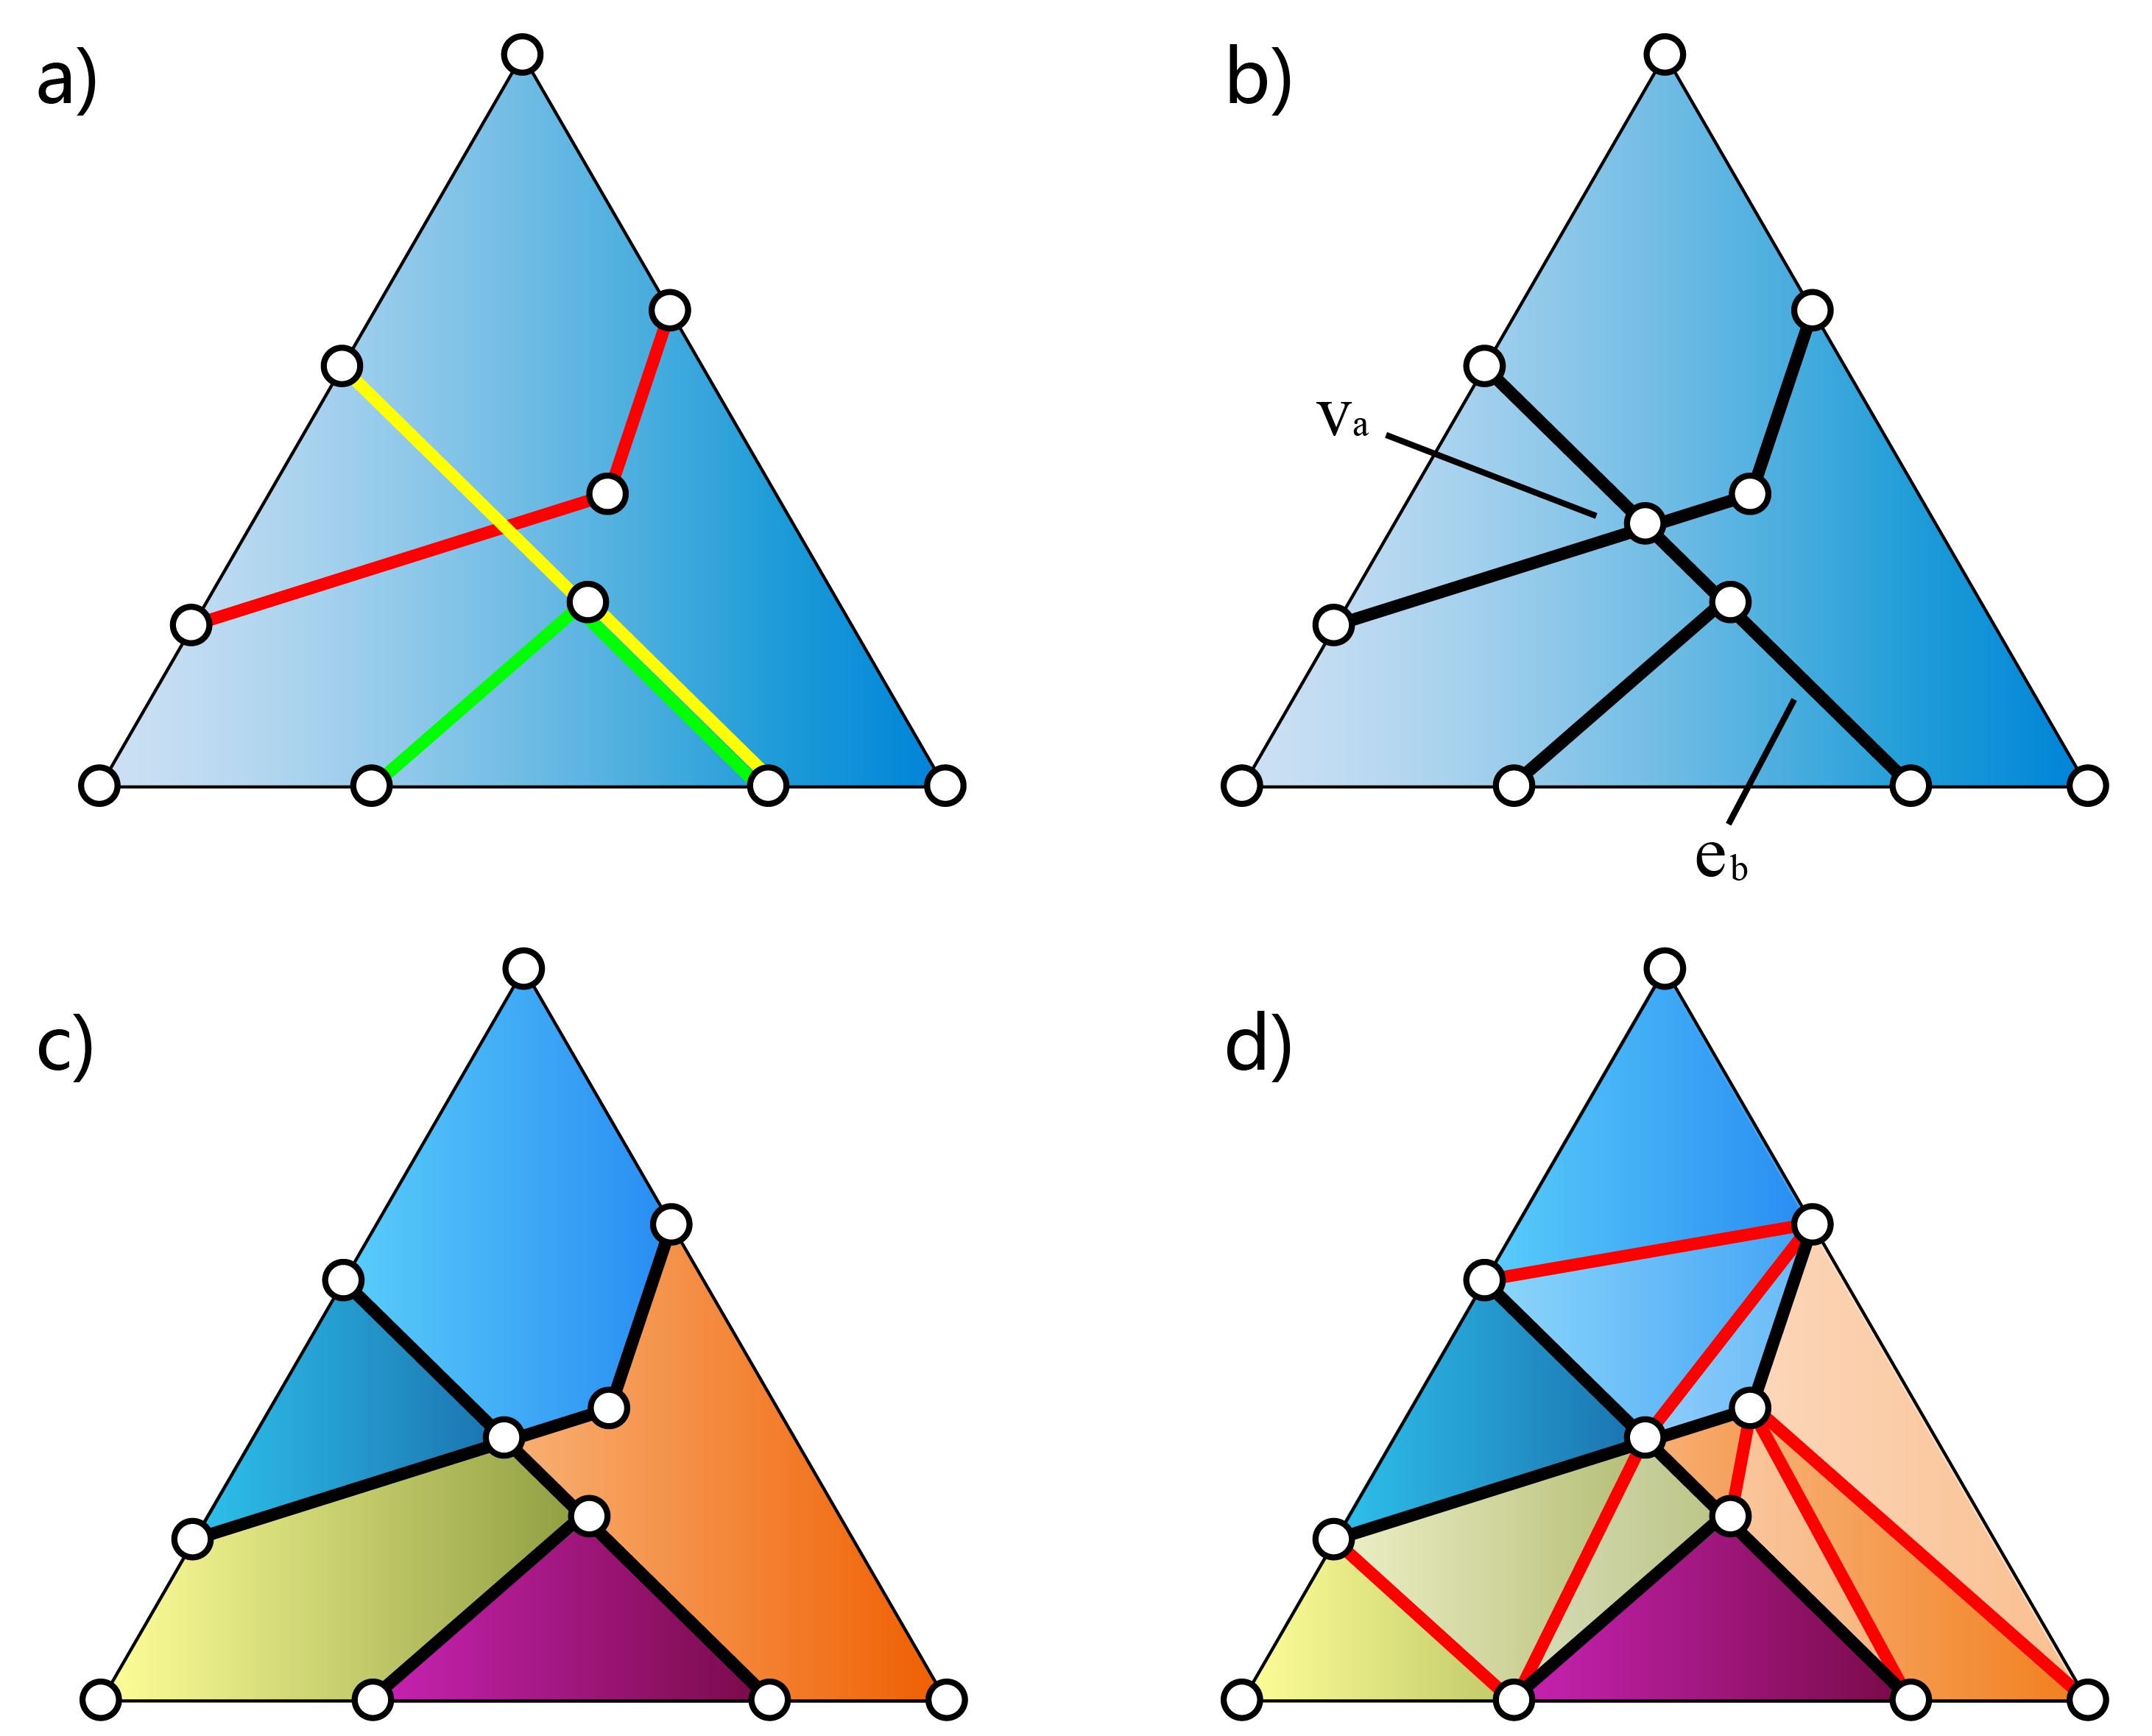
\includegraphics[width=3.5in]{boolean-04}
\caption{a) Different colors indicate that the intersections originate from different meshes. The yellow and red intersections intersect at a point. The yellow intersection overlaps with the green intersection. b) After refinement, we introduce a new vertex $\bm{v}_a$, and merge overlapping intersections into a single edge $\bm{e}_b$. c) Our tessellation method does not guarantee that all of the faces are triangular. d) If triangulation is performed, new edges (red lines) are introduced and double-precision is not enough to hold the plane coefficients of their P-reps.}
\label{fig:iisect}
\end{figure}


In our method we first perform intersection refinement to ensure that intersections intersect each other only on end points. After that, we perform our minimal tessellation based on \emph{tess-graph}, a graph-like description of the intersections on a given face.

\subsection{Intersection Refinement}

\label{sec:refine}

Intersection vertices can be introduced by the intersection of three triangles, in addition to intersections between an edge and a triangle. Triangle-triangle intersection tests only compute the latter. Thus, it is necessary to refine these triangle-triangle intersections before the final tessellation.

Intersection refinement is performed on the scope of each intersecting triangle. For triangle face $t$, we collect all of the intersections on $t$ as a set $\bm{\Gamma}(t)$ and refine them together. We also include the three edges of $t$ in $\bm{\Gamma}(t)$, because the edges are also involved in the step of subfaces extraction. In $\bm{\Gamma}(t)$, the three edges are represented by PBI-reps. The neighboring faces $\mathcal{N}$ are set as $N/A$ because they do not have a neighboring face. Other PBI-rep components can be determined by the P-reps of the edges. The refinement of $\bm{\Gamma}(t)$ is done using only plane-based geometric predicates, in the following three steps.


\vspace{0.5em}
\noindent \textbf{Coincidence elimination}~~~~
We merge coincidence intersections that have the same end points. Intersections are undirected, so intersections with inverse end points are also coincident. The PBI-rep of the merged intersection is inherited from either of the original intersections, except for the neighboring faces $\mathcal{N}$. The neighboring faces of the merge intersection is the union of all the neighboring faces of original ones. It means from now on, an intersection may have neighboring faces from different primitives.

\vspace{0.5em}
%Intersection refinement is performed locally
\begin{wrapfigure}{r}[0in]{0in}
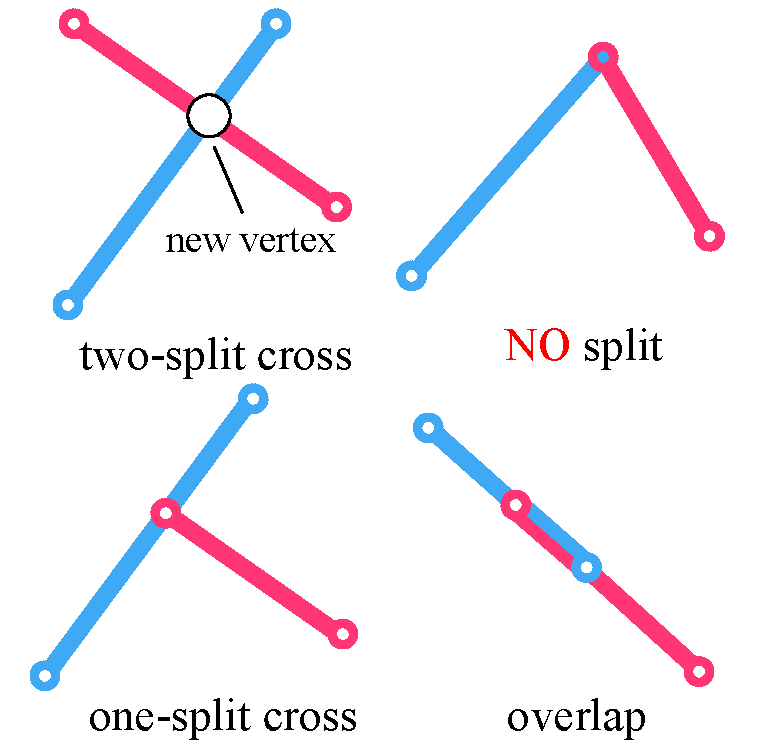
\includegraphics[width=1.6 in]{resolve}
%\caption{Plane-based representation of triangle}
\end{wrapfigure}
\noindent\textbf{Intersection resolving}~~~~
Each pair of intersections is tested if they intersect in any location other than end points. The test intersections should be from different primitives, since primitive inputs are free of self-intersecting. When two intersections intersect, at least one of them is split. New vertices may be introduced, whose P-reps are intersections between the common plane and the two $\bm{P}_ext$ of the PBI-reps. Because one intersection may be in contact with more than one other intersection, this splitting is deferred until all of the splitting points are found. The PBI-reps of the split segments inherit that of their father's, except for $\bm{P}_0, \bm{P}_1$, since the split segments have different end points.

\vspace{0.5em}
\noindent \textbf{Coincidence elimination (revisited)}~~~~
If two intersections are collinear, resolving their overlap may produce new coincident intersections. Therefore, the first step of the process is repeated here.

\subsection{Tessellation by Tess-Graph}
\label{sec:tess}

To perform tessellation and extract subfaces, we use tess-graph, which is the graph description of the tessellated face topology. For each intersecting triangle face, we construct a tess-graph according to the refined set of intersections. Nodes of the tess-graph represent the end points of intersections, and connections between nodes represent intersections. The construction of a tess-graph is straightforward, and readers should be able to determine the details.


After the tess-graph is constructed, we extract subfaces by   valid loops. A valid loop is a loop in tess-graph which satisfy two criteria: 1) the direction of the loop should correspond with the face normal, and 2) consecutive connections on the loop should be adjacent by circular order. Each valid loop corresponds to an intersection-free face. After all of the valid loops are determined from the tess-graph, the corresponding face is tessellated (see Fig. \ref{fig:cadj}). To facilitate face classification, we also store neighboring faces in the edges of the new faces. Because the edges have one-to-one correspondence to the connections in tess-graph , and the connections have one-to-one correspondence to the PBI-reps, the neighboring faces of edges is determined from the corresponding PBI-reps.

\begin{figure}[t]
\centering
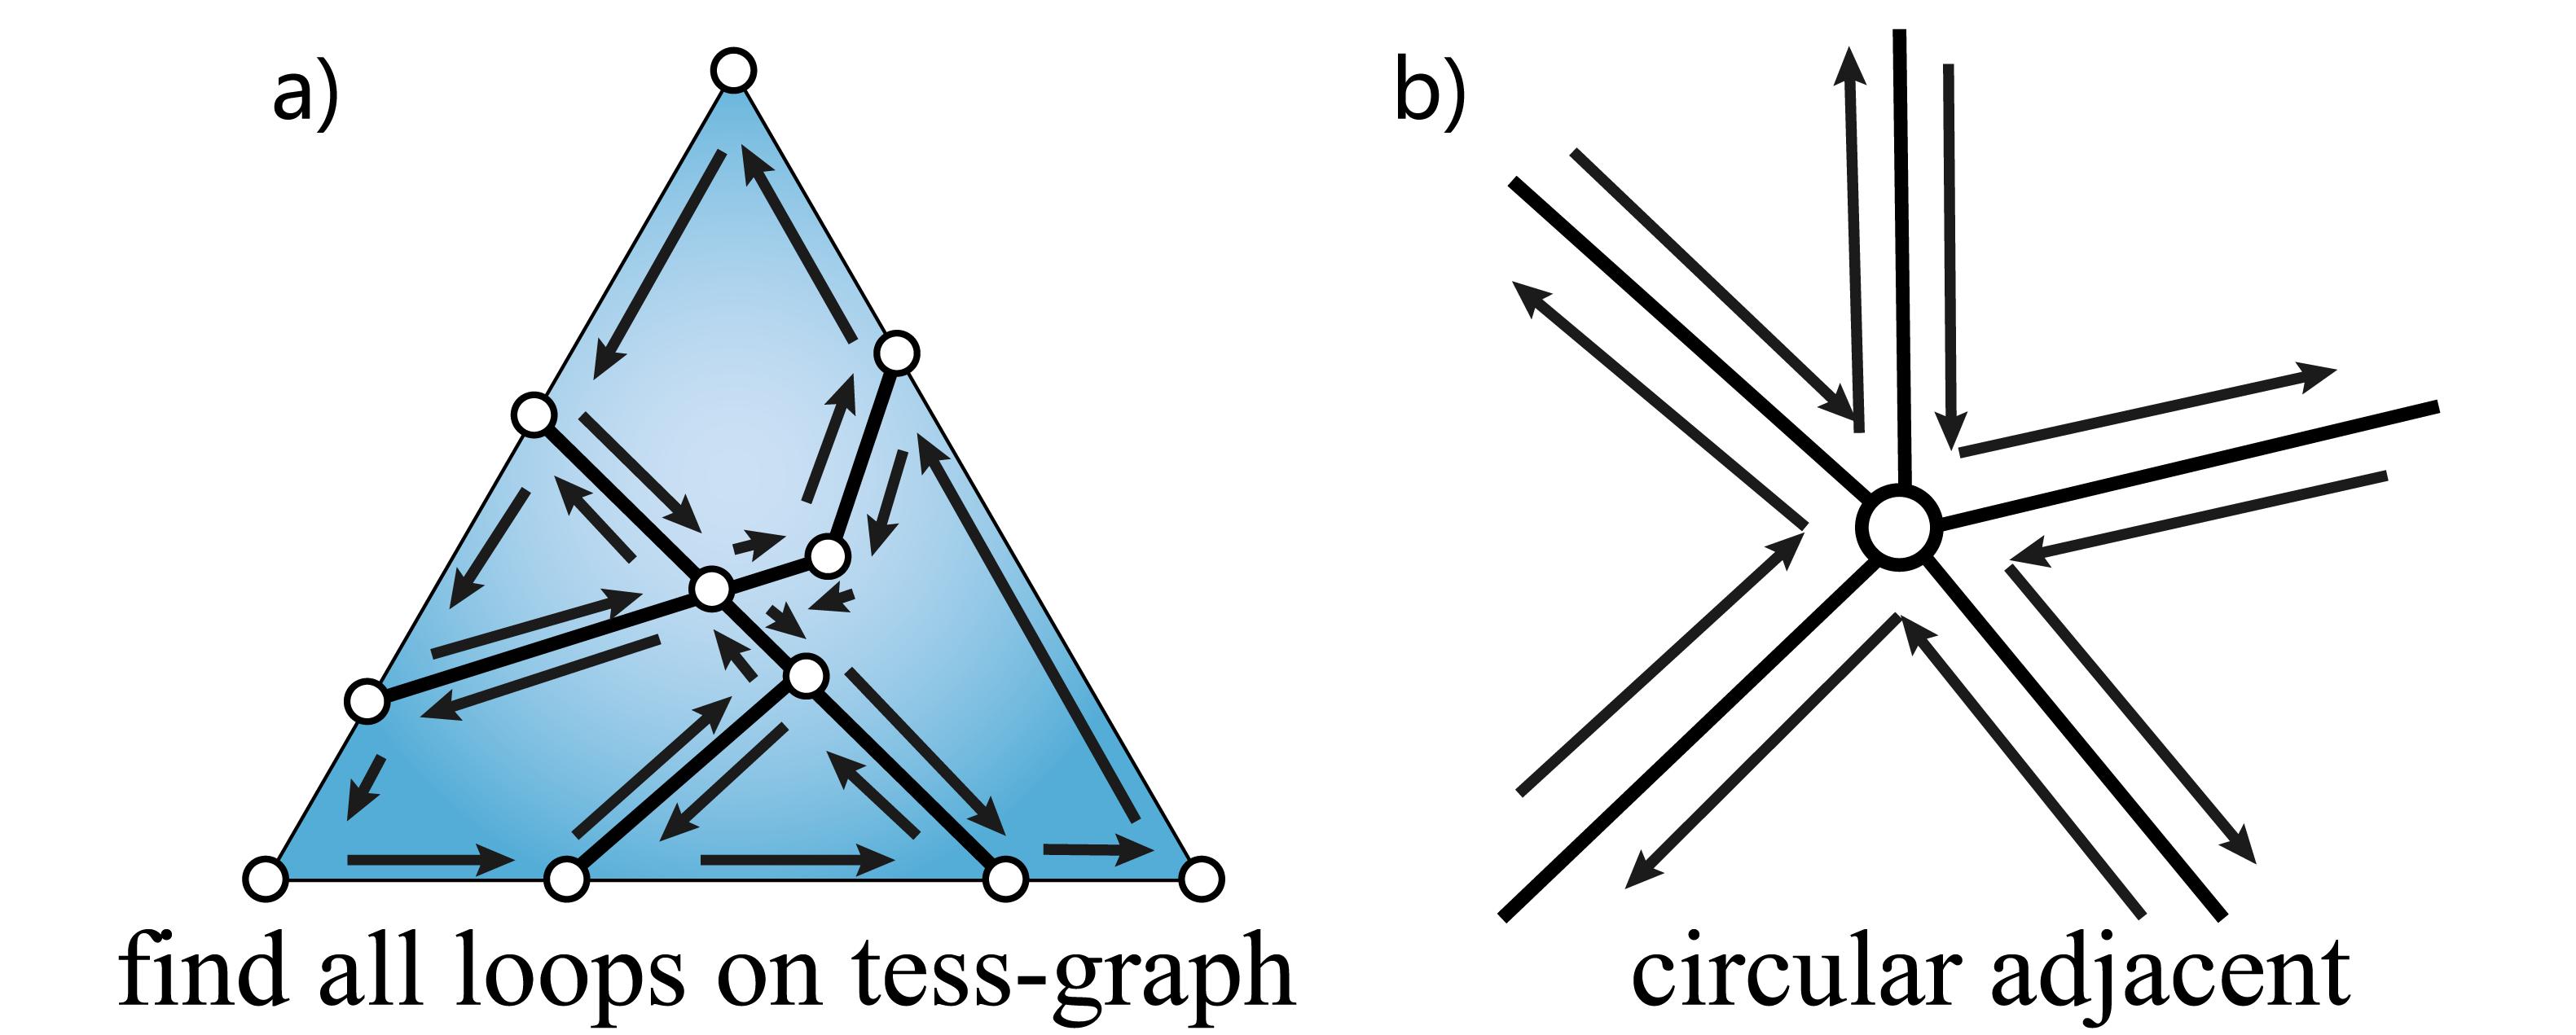
\includegraphics[width=3in]{boolean-05}
\caption{a) To tessellate a triangle, we find all of the valid loops on a tess-graph. The direction of the loops must be coherent with the triangle normal (assuming here that the normal points to the outside of the paper). b) Each circular adjacent edge pair is an angle of the tessellated polygon.}
\label{fig:cadj}
\end{figure}



\section{Face Classification}

\label{sec:classification}
%We traverse each face in the intersection-free meshes, and classify which one belongs to the final mesh. Classification is done by evaluating the label vector $\bm{\Lambda}$ of each face. The basic idea of our classification method is to utilize the space coherence of face label vectors to share the classification results among neighboring faces. Also, because we store the neighborhood information in the edges which intersect other meshes, the search space of point-in-polyhedron test is limited to only a few faces. It makes the label computation very fast. Finally, by using P-reps, our classification method is exact can deal with any degenerate cases.

We traverse each face of the primitives, and determine which belong to the final mesh. The faces are classified by evaluating their inclusion label vector. Our classification method utilizes the space coherence of the label vectors, and shares the classification results among neighboring faces. Because we store the neighboring faces in the edges where intersections occur, the label computation is very fast according to the orientation of these neighboring faces.


Intersection-free meshes facilitate this process by accelerating the label propagation. From adjacent faces $\bm{s}_1$ and $\bm{s}_2$, it is straightforward to determine whether $\bm{\Lambda}(\bm{s}_1)$ and $\bm{\Lambda}(\bm{s}_2)$ are different. The two label vectors are the same unless the shared edge $\bm{e}_{12}$ lies on the boundary of another mesh. In that cases, neighborhood information, say, $\bm{\mathcal{N}}(\bm{e}_{12}) = \{\mathcal{N}_k\}$, is stored on $\bm{e}_{12}$. Here we use $\bm{\mathcal{N}}$ to indicate that the edge may have more than one neighborhood (see \S\ref{sec:refine}). The neighborhood information indicates which components of the label vector differ between $\bm{s}_1$ and $\bm{s}_2$. If there is neighborhood information from mesh $M_x$, the $x^{th}$ labels $\lambda_x(\bm{s}_1)$ and $\lambda_x(\bm{s}_2)$ differ, and can be computed efficiently and exactly with respect to that neighborhood. We outline our classification method in Algorithm \ref{code:floodfill}.

%The space coherence of label vectors means neighboring faces may have the same label vector, or most components of label vectors. Therefore, we start from a seed face $\bm{s}_0$ with its label vector $\bm{\Lambda}(\bm{s}_0)$ known, and propagate to other faces in a flood-filling manner. The trace of label propagation is:

% The space coherence of label vectors means that neighboring faces may have the same label vector, or most of the components of the label vectors. Therefore, we start from a seed face $\bm{s}_0$ with a known label vector $\bm{\Lambda}(\bm{s}_0)$, and propagate the label to other faces in a flood-filling manner. The trace of the label propagation is:

% \begin{equation}
% \label{eq:trace}
% \bm{s}_0\to \bm{s}_1\to \bm{s}_2\to \bm{s}_3\to ...
% \end{equation}



%Intersection-free meshes facilitate this process by accelerating the label propagation. From adjacent faces s1 and s2, it is straightforward to determine whether

\begin{algorithm}[ht]
\caption{Fast Face Classification}
\label{code:floodfill}
\textbf{Input: } Intersection-free hybrid meshes, boolean function $f$

\textbf{Output: } Classification $f(\bm{\Lambda}(\bm{s}_i))$ for all faces $\bm{s}_i$


\begin{algorithmic}[1]
\State Select a proper seed face $\bm{s}_0$
\State Compute the seed label vector $\boldsymbol{\Lambda}(\bm{s}_0)$
\State \Call{propagate} { $\bm{s}_0$ , $\boldsymbol{\Lambda}(\bm{s}_0)$}
\State
\Function{propagate}{ $\bm{s}$ , $\boldsymbol{\Lambda}(\bm{s})$}
    \State Compute $f(\boldsymbol{\Lambda}(\bm{s}))$
    \For {each neighboring face $\bm{s}_{s, i}$}
        \If {$\bm{s}_i$ has been classified}
            \State continue
        \EndIf
        \If {there are PBI-reps ${\bm{\mathcal{I}}}_k$ on $\bm{e}(\bm{s}_{s, i}, s)$}
            \State compute $\boldsymbol{\Lambda}(\bm{s}_{s, i})$ by $\boldsymbol{\Lambda}(\bm{s})$ and ${\bm{\mathcal{I}}}_k$
            \State \Call{propagate} { $\bm{s}_{s, i}$ , $\boldsymbol{\Lambda}(\bm{s}_{s, i})$}
        \Else
            \State \Call{propagate} { $\bm{s}_{s, i}$ , $\boldsymbol{\Lambda}(\bm{s})$}
        \EndIf
    \EndFor
\EndFunction
\end{algorithmic}
\end{algorithm}


\subsection{label Propagation}
\label{sec:propagation}


%Meshes consist of vertices, edges and faces. Classification is required to perform on the face level. However, polyhedron-in-out test is performed based on points. Gaps exist between the them. Conventionally, face barycenter is used to compute the label of the whole face. This is because in intersection-free meshes, face is classified as a whole, and every face inner point will have the same label as the face's. However, the computation of inner point coordinates requires geometry construction, which introduces errors without exact arithmetic. Therefore, we use the face (or subface) vertices instead, whose exact representations are known, for label computation.

Meshes consist of vertices, edges and faces. It is necessary to perform classification at the face level. However, polyhedron-in-out tests are performed on points, where gaps exist between them. Conventionally, the face barycenter is used to compute the label of the whole face because in intersection-free meshes, the face is classified as a whole, and every inner point of the face will have the same label as the whole face. However, the computation of inner point coordinates requires geometric constructions, which introduce errors unless exact arithmetic can be used. Therefore, we use the face (or subface) vertices instead, the exact representations of which are known, for label computation.

\begin{wrapfigure}{r}[0in]{0in}
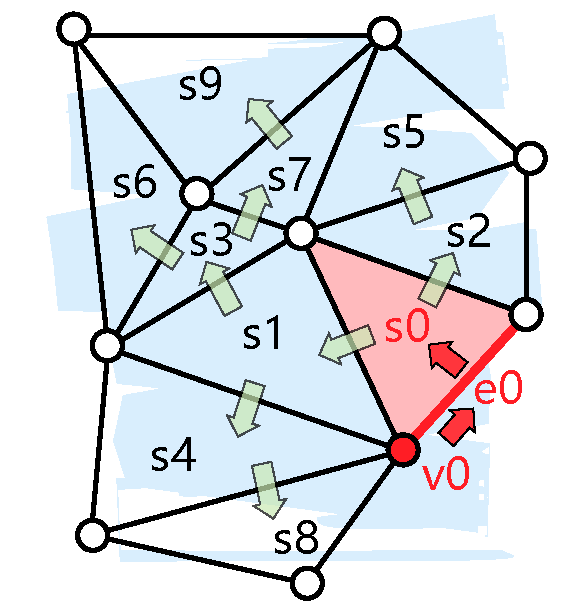
\includegraphics[width=1.3 in]{propagate}
\end{wrapfigure}


%However, there are two gaps between face label and face vertex label. First, the label of vertex does not always equal to label of face. Second, face label has two extra classes in $on$ case---$same$ and $oppo$, because the face has its orientation.


\begin{figure}[t]
\centering
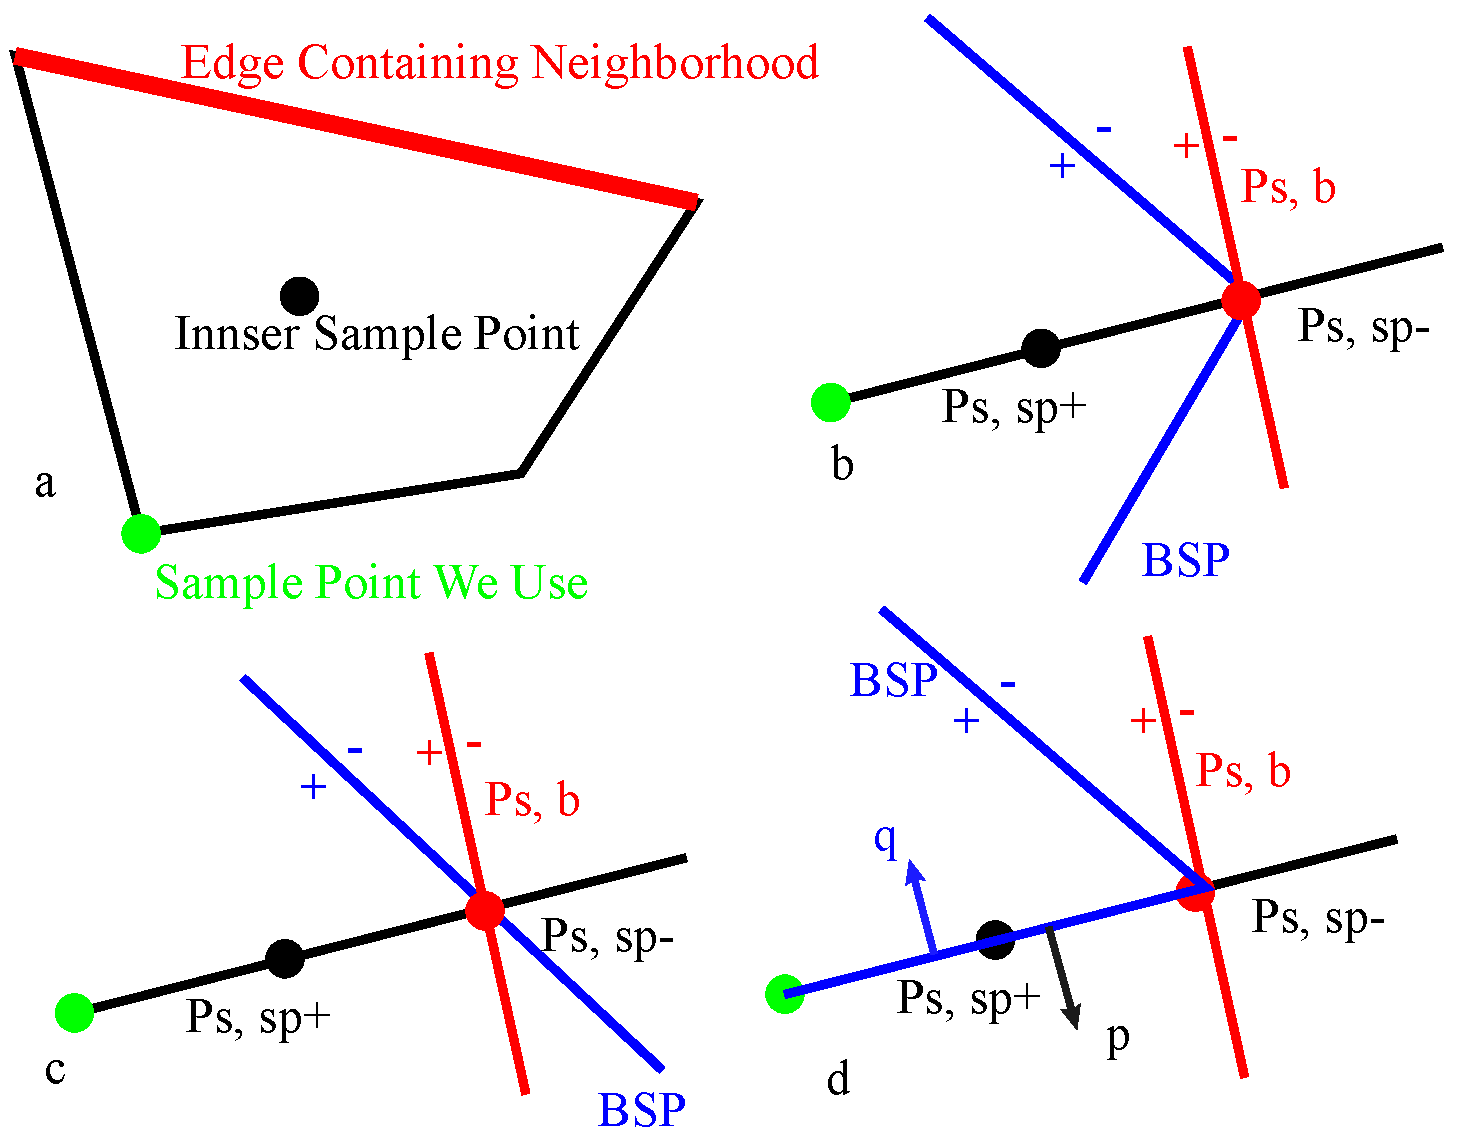
\includegraphics[width=3in]{bsps}
\caption{a) Because the inner sample point includes geometric constructions, we choose the face vertex (orange) instead to compute the face label. b-d) Different types of classification. The simple structure of the neighborhood BSP guarantees the same classification result for all of the points on $\bm{p}_{\bm{s}, sp}^+$. In d), the classification result is $on$ so it is necessary to determine the orientation from the normal of the BSP splitting plane $q$ and the face normal $p$. In this cases, the label should be $oppo$ because $p$ and $q$ are opposite.}
% a) Because the
\label{fig:bsps}
\end{figure}


However, there are two discrepancies between the face and face vertex labels. First, the vertex label is not always equal to the face label. Second, the face label has two extra classes in the $on$ case��$same$ and $oppo$��because the face has an orientation.

%To overcome the gaps, we rewrite our label trace (\ref{eq:trace}) in finer granularity. In the beginning, we start from a seed vertex $\bm{v}_0$ on seed face $\bm{s}_0$. We assume label vector $\bm{\Lambda}(\bm{v}_0)$ is known. Then we use $\bm{\Lambda}(\bm{v}_0)$ to compute $\bm{\Lambda}(\bm{s}_0)$. In addition, we add an optional edge layer into the trace. Then it changes to:

To deal with these discrepancies, the label trace (\ref{eq:trace}) is modified for finer granularity. We start from a seed vertex $\bm{v}_0$ on a seed face $\bm{s}_0$. We assume that the label vector $\bm{\Lambda}(\bm{v}_0)$ is known. Then we use $\bm{\Lambda}(\bm{v}_0)$ to compute $\bm{\Lambda}(\bm{s}_0)$. In addition, we add an optional edge layer into the trace:

\begin{equation}
\bm{v}_0\to \bm{e}_0\to \bm{s}_0\to (\bm{e}_1)\to \bm{s}_1\to (\bm{e}_2)\to \bm{s}_2\to ...,
\end{equation}
%where $\bm{v}$ and $\bm{e}$ are the vertex and edge, respectively. The bracket indicates that propagating to the edge is optional, because if the edge does not contain neighborhood information the labels on the two side are the same and we do not need to propagate to the edge. We find that there are three kinds of basic operations in the trace: $\bm{v}_{\bm{e}}\to \bm{e}$, $\bm{e}_{\bm{s}}\to \bm{s}$ and $\bm{s}\to \bm{e}_{\bm{s}}$, where $\bm{v}_{\bm{e}}$ means the end point of $\bm{e}$, and $\bm{e}_{\bm{s}}$ means the edge of $\bm{s}$.
where $\bm{v}$ and $\bm{e}$ are the vertex and edge, respectively. The bracket indicates that propagating to the edge is optional, because if the edge does not contain neighborhood information the labels on either side are the same, so we do not need to propagate to the edge. There are three basic operations in the trace: $\bm{v}_{\bm{e}}\to \bm{e}$, $\bm{e}_{\bm{s}}\to \bm{s}$ and $\bm{s}\to \bm{e}_{\bm{s}}$, where $\bm{v}_{\bm{e}}$ is the end point of $\bm{e}$, and $\bm{e}_{\bm{s}}$ is the edge of $\bm{s}$.

%Given the partial order $on \succ in$ and $on \succ out$, our key observation is that the following relation always stands for labels within intersection-free meshes:
Given the partial orders $on \succ in$ and $on \succ out$, the following relationship is true for labels within intersection-free meshes:

\begin{equation}
\label{eq:porder}
\lambda_k(\bm{v}_{\bm{e}_{\bm{s}}}) \succeq \lambda_k(\bm{e}_{\bm{s}}) \succeq \lambda_k(\bm{s}),
\end{equation}
where $\lambda_k(x)$ is the label of $x$ for a certain primitive $M_k$. This relationship can be inferred from the continuous space assumption and the definition of intersection-free mesh*. It indicates that when we perform $\bm{v}_{\bm{e}}\to \bm{e}$ and $\bm{e}_{\bm{s}}\to \bm{s}$, from a low-dimension to a high-dimension, we decide whether the $on$ label changes to $in$ or $out$, or remains $on$. When we perform $\bm{s}\to \bm{e}_{\bm{s}}$, we decide whether $in$ and $out$ labels are changed to $on$. In addition, when considering the orientation of the face, we also need to determine whether the $on$ labels change to $same$ or $oppo$ during the $\bm{e}_{\bm{s}}\to \bm{s}$ operation.

%where

\vspace{0.5em}
\noindent\textbf{$\bm{s\to \bm{e}_{\bm{s}}}$}~~~~ We need to determine which labels change to $on$. We know that when $\lambda_k(\bm{e}_{\bm{s}})=on$, there will be neighborhood information related to mesh $M_k$ stored on $\bm{e}_{\bm{s}}$. Therefore, in this operation, we need to traverse all of the neighborhoods of $\bm{e}_{\bm{s}}$ and change the corresponding labels to $on$.

%s


\vspace{0.5em}
\noindent\textbf{$\bm{\bm{e}_{\bm{s}}\to \bm{s}}$}~~~~From eq. \ref{eq:porder}, we know that if $\lambda_k(\bm{e}_{\bm{s}}) \neq on$, then $\lambda_k(\bm{e}_{\bm{s}})=\lambda_k(\bm{s})$. Conversely, when $\lambda_k(\bm{e}_{\bm{s}}) = on$, $\lambda_k(\bm{s})$ can be determined using neighborhood information related to $M_k$. The neighborhood of $M_k$ can be either a face or a set of faces from the mesh $M_k$.  We can build a trivial BSP \cite{thibault1987set} using these faces. The BSP can be used to compute $\lambda_k(\bm{s})$ if a point can be sampled from $\bm{s} \cap \bm{U}(\bm{e}_{\bm{s}})$, where $\bm{U}(\bm{e}_{\bm{s}})$ is the neighborhood space of $\bm{e}_{\bm{s}}$. Unfortunately, we cannot guarantee that such a point can be found with precise coordinates.

%
\vspace{0.5em}
\begin{wrapfigure}{r}[0in]{0in}
 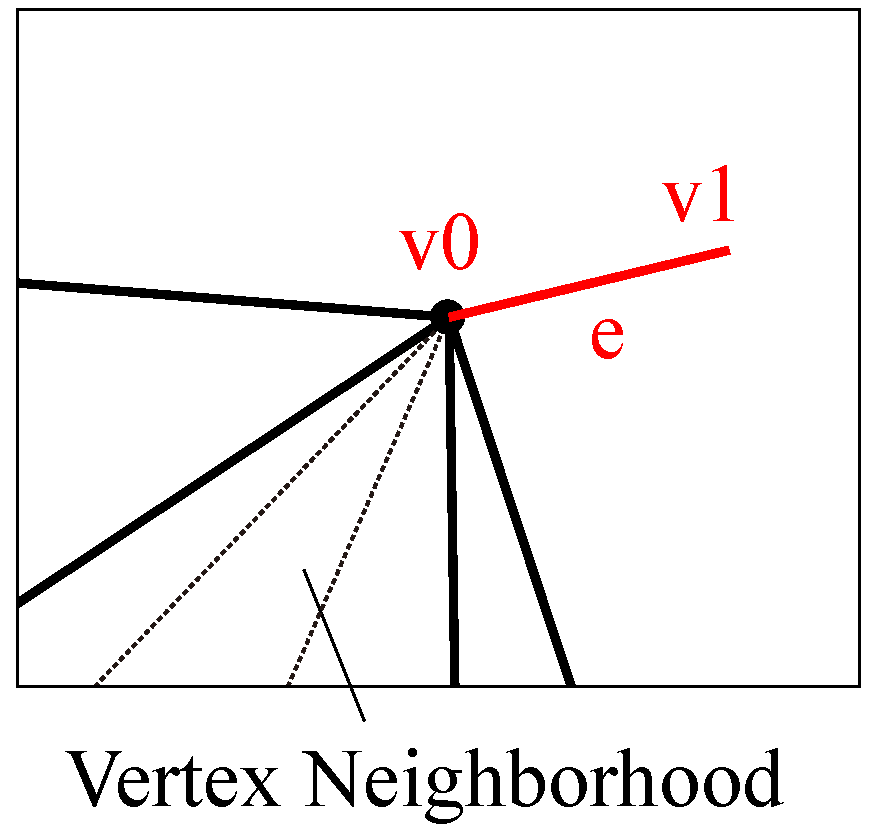
\includegraphics[width=1.3 in]{vneighbor}
\end{wrapfigure}
Our BSP is constructed from a single face, or a set of faces sharing the same edge. This BSP is sufficiently simple that the labels $\lambda_k$ of all of the points on the half plane $\bm{p}_{\bm{s}, sp}^+$ are identical. Here $\bm{p}_{\bm{s}, sp}^+$ is half of the supporting plane of $\bm{s}$ that lies on the positive side of the bounding plane $\bm{p}_{\bm{s}, b}^{\bm{e}_{\bm{s}}}$ (Fig. \ref{fig:bsps}). Since $\bm{p}_{\bm{s}, sp}^+ \cap \bm{s} \neq \varnothing$, we can compute $\lambda_k(\bm{s})$ by determining $\lambda_k(\bm{v}_x, \bm{v}_x \in \bm{p}_{\bm{s}, sp}^+)$. For polygons, at least one corner point lies on $\bm{p}_{\bm{s}, sp}^+$, and the exact coordinates of the corner point are known. That corner point is used as $\bm{v}_x$. In addition, we assign each BSP splitting plane a normal from the normal of the triangle it contains, from which we can decide the orientation ($same$ or $oppo$) when $\lambda_k(\bm{s})=on$.

%Our BSP is constructed from a single face, or a set of faces sharing the same edge. This BSP is sufficiently simple that the labels

\noindent\textbf{$\bm{\bm{v}_{\bm{e}}\to e}$}~~~~If $\lambda_k(\bm{v}_{\bm{e}})=on$, we first check whether $\lambda_k(\bm{e}) = on$, by checking whether there is neighborhood information related to $M_k$ on $\bm{e}$. If not, we need to find where $\bm{v}_{\bm{e}}$ lies on $M_k$. This is straightforward because the intersection-free meshes contain geometric connectivity information. We can consider the connectivity information as the vertex version of neighborhood information, and the same BSP-based classification method is used in ${\bm{e}_{\bm{s}}\to \bm{s}}$ can be used to determine the high dimension label $\lambda_k(\bm{e})$. We use the other end point $\bm{v}'_{\bm{e}}$ as the sample point for the BSP classification.

%ve


\subsection{Acceleration by Caching}
\label{sec:acc}
%If the CSG tree is large with hundreds of primitive nodes, computing $\lambda_f(\bm{s}_i)$ from $\boldsymbol{\Lambda}(\bm{s}_i)$ for every face $\bm{s}_i$ can be costly. Thanks to the label space coherence, we can save the computation time by caching the evaluation result during flood-filling.

If the CSG tree is large, with hundreds of primitive nodes, computing $\lambda_f(\bm{s}_i)$ from $\boldsymbol{\Lambda}(\bm{s}_i)$ for every face ($\bm{s}_i$) can be costly. However, using label space coherence, we can reduce the computation time by caching the evaluation results during flood-filling.

%The basic cache strategy is to cache final result, that is, the value of $\lambda_f(\bm{s}_i)$. We know label vector will not change if there is no intersection edge during propagation. That means the final classification $\lambda_f(\bm{s}_i)$ will not change, too. Thus, those faces sharing the same label vector can be classified as a whole.

The basic caching strategy is to cache the final result, that is, the value of $\lambda_f(\bm{s}_i)$. We know that the label vector will not change if there is no intersection edge encountered during propagation. Therefore, the final classification $\lambda_f(\bm{s}_i)$ will not change either. Thus, faces which share the same label vector can be classified as a set.

%Also, we can perform intermediate results cache. We noticed that the boolean expression can be simplified if some components of $\bm{\Lambda}(\bm{s}_i)$ is fixed. For example, assume we have a boolean expression $f = M_1\cup (M_2\cap M_3-M_4)$. Given the values of two labels $\lambda_1(\bm{s}_i)=out$, $\lambda_2(\bm{s}_i)=in$, the expression can be rewritten as $f(\lambda_1=out, \lambda_2=in)=out\cup (in\cap M_3-M_4)$. Using the combination rules we can simplify the expression as $f(\lambda_1=out, \lambda_2=in)=P_3-P_4$. Because for a large CSG, a certain mesh often intersects with only a few other meshes $\Theta= \{M_{n_1}, M_{n_2}, \cdots, M_{n_x}\}$. That means all the faces in this mesh has the same labels against $M_{i} \notin \Theta(M_k)$. Therefore, we can first determine these fixed labels and simplify the boolean function, and then use simplified one to compute the final label for each faces in this mesh.

We can also perform an intermediate results cache. The boolean expression can be simplified if some components of $\bm{\Lambda}(\bm{s}_i)$) are fixed. For example, assume we have a boolean expression $f = M_1\cup (M_2\cap M_3-M_4)$. Given the values of two labels $\lambda_1(\bm{s}_i)=out$, $\lambda_2(\bm{s}_i)=in$, the expression can be rewritten as $f(\lambda_1=out, \lambda_2=in)=out\cup (in\cap M_3-M_4)$. Using the combination rules, we can simplify the expression to $f(\lambda_1=out, \lambda_2=in)=M_3-M_4$. In a large CSG, a given mesh often intersects with only a few other meshes $\Theta= \{M_{n_1}, M_{n_2}, \cdots, M_{n_x}\}$. Thus, all of the faces in this mesh have the same labels for $M_{i} \notin \Theta(M_k)$. Therefore, if we can determine the fixed labels and simplify the boolean function, then we compute the final label for each face in this mesh.


\iffalse
\subsection{Tessellating on Classification}
We find for a CSG with many meshes, a large percentage of intersections are invalid (see \S\ref{sec:degenerate} for 'invalid'). Tessellation according to these invalid intersections is not necessary. To avoid unnecessary tessellation, we can give an early prediction of which intersections are invalid by intersections information of faces, but have to embed the tessellation stage into the classification stage, which we call it 'tessellating on classification'.

In most situations, a certain faces $\bm{s}$ only intersect with a few other meshes $\Theta(\bm{s})$. We can use the same cache strategy in \S\ref{sec:acc} to shrink the original CSG into a smaller one by the common labels of $\{P_i\}\backslash\Theta(\bm{s})$, where $\{P_i\}$ means all the primitive meshes. After the shrinking, the primitive meshes of the CSG must be from $\Theta(\bm{s})$. If any mesh in $\Theta(\bm{s})$ does not appear in the shrinked CSG, it means the label of that mesh does not change the classification result, which in another word, intersections on $\bm{s}$ from that mesh are invalid and do not affect the classification of any subfaces of $\bm{s}$. If the shrinked CSG is trivial which does not contain any primitives, it means $\bm{s}$ does not need tessellation. In this way, we save the computation time, and simplify the topology of the final result mesh. Because we can only shrink the CSG for $\bm{s}$ when we classify it---before that the labels of meshes from $\{P_i\}\backslash\Theta(\bm{s})$ are not known---we do not perform tessellation until we do the classification.
\fi

\iffalse

\subsection{Implementation}

\label{sec:individual}

Feito et. al. \cite{feito2013fast} had noticed that intersection neighborhood can be used for fast classification of faces around that intersection. According to their method, faces adjacent to intersection have neighbors from other primitive(\bm{s}) that define the position and orientation for each other, by which the indicators are determined. However, Feito et. al. did not give detail description of how to implement an exact and robust classification. Their implementation of using vertex coordinates might misclassify faces by numeric errors and fail in degenerate cases. Because geometry connectivity is used, local misclassification can be spread to the neighborhoods, leading to errors in wide ranges.

We develop an classification method that is unconditionally robust and exact based on the idea of using intersection neighborhood information. The neighborhood information is stored in the context component of I-reps during previous stages . In the following, we discuss the conditions that the face to be classified is a triangle. If the face is not a triangle, we select a triangle slice of the face instead, as the whole face is guaranteed to be classified together. Note that the chosen slice should contain the edge where the I-reps lie, by which we compute the new indicators.

Given a face $t_i$ to be classified and an I-rep $\boldsymbol\Gamma$ of intersection on one of $t_i$'s edge, we denote the three corners it as $\bm{v}_{b*}^{0}(t_i), \bm{v}_{b*}^{1}(t_i), \bm{v}_b^2(t_i),$ where the subscript $*$ means the vertices are on the edge where $\boldsymbol\Gamma$ lies. We also denote the context component of $\boldsymbol\Gamma$ as $C_{P_h \backslash P_j}$, meaning $t_i$ is from primitive $M_j$ and intersects primitive $M_h$. From previous discussion (section \ref{sec:ir}){\color{red}{may be more than one}}, we know there are two types of intersection context---face neighborhood and edge neighborhood. In both conditions, the one or two faces involving in the context split the space into two in and out space by its (their) orientation(\bm{s}). We will see that under such division (denoted as $\boldsymbol{D}(C_{P_h \backslash P_j})$), we can compute $\lambda(t_i, P_j)$ exactly.

Since the faces involving in $C_{P_h \backslash P_j}$ is part of primitive $M_j$, the space division $\boldsymbol{D}(C_{P_h \backslash P_j})$ is homogeneous with the space division by $M_j$ in neighborhood of $\bm{\mathcal{I}}$. The basic idea is to choose one point $\bm{v}_x(t_i)$ on $t_i$ close enough to $\bm{\mathcal{I}}$ to compute $\lambda(\bm{v}_x(t_i), P_j)$, and then compute $\lambda(t_i, P_j)$ accordingly. However, the problem is that we cannot find such a $\bm{v}_x(t_i)$ that can be represented exactly, which means robust classification cannot be performed. Fortunately, we observe that we can choose $\bm{v}_b^2(t_i)$, which is not so close to $\bm{\mathcal{I}}$ instead. To illustrate, assume there is another point $\bm{v}_{x'}(t_i)$ inside of $t_i$ that is very close to $\bm{v}_b^2(t_i)$ ({\color{red}{Fig. x}}). Because all inner points of $t_i$ have the same indicator, $\lambda(\bm{v}_x(t_i), P_j) = \lambda(\bm{v}_{x'}(t_i), P_j)$. On the other hand, we find that $\lambda(\bm{v}_{x'}(t_i), P_j)$ and $\lambda(\bm{v}_b^2(t_i), P_j)$ are always equal under division $\boldsymbol{D}(C_{P_h \backslash P_j})$ ({\color{red}{see Appendix \ref{app:profind}}}). Therefore, $\lambda(\bm{v}_b^2(t_i), P_j)$ is equal to $\lambda(\bm{v}_x(t_i), P_j)$ under $\boldsymbol{D}(C_{P_h \backslash P_j})$, and are coherent with $\lambda(t_i, P_j)$ under the division of whole primitive $M_j$. One additional thing is that when $\lambda(\bm{v}_2(t_i), P_j)=on$, then $\lambda(t_i, P_j)$ can be either $same$ or $oppo$. The normal orientation test have to be performed to eliminate such ambiguity.

\fi

\section{Results and Discussion}


\begin{figure}[t]
\centering
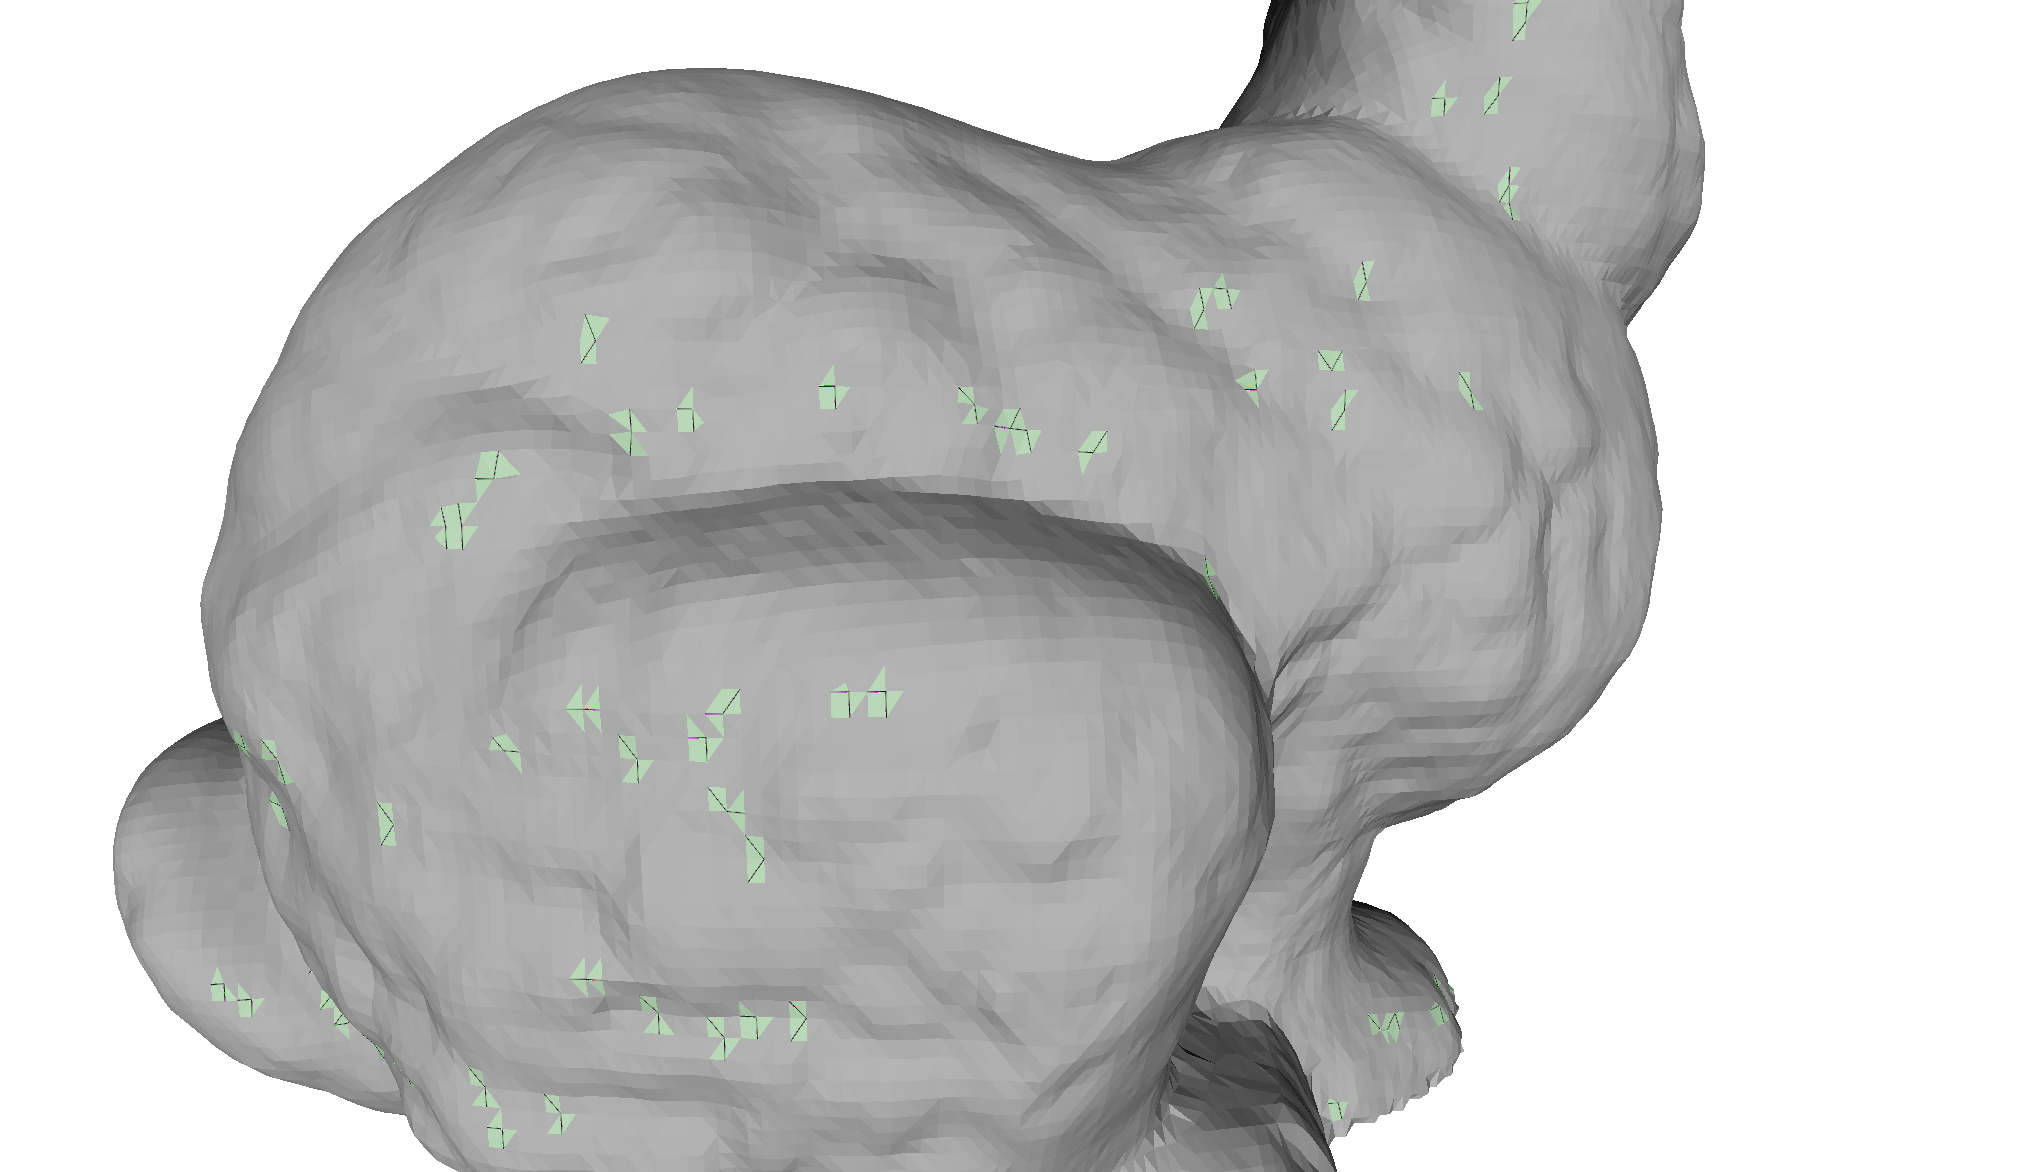
\includegraphics[width=3in]{perturb}
\caption{After perturbation, the self-union of \emph{Bunny} with QuickCSG still suffers from topology problem. The green boundary faces indicate topological deficiencies.}
%
\label{fig:boundaryedge}
\end{figure}

\begin{figure}[t]
\centering
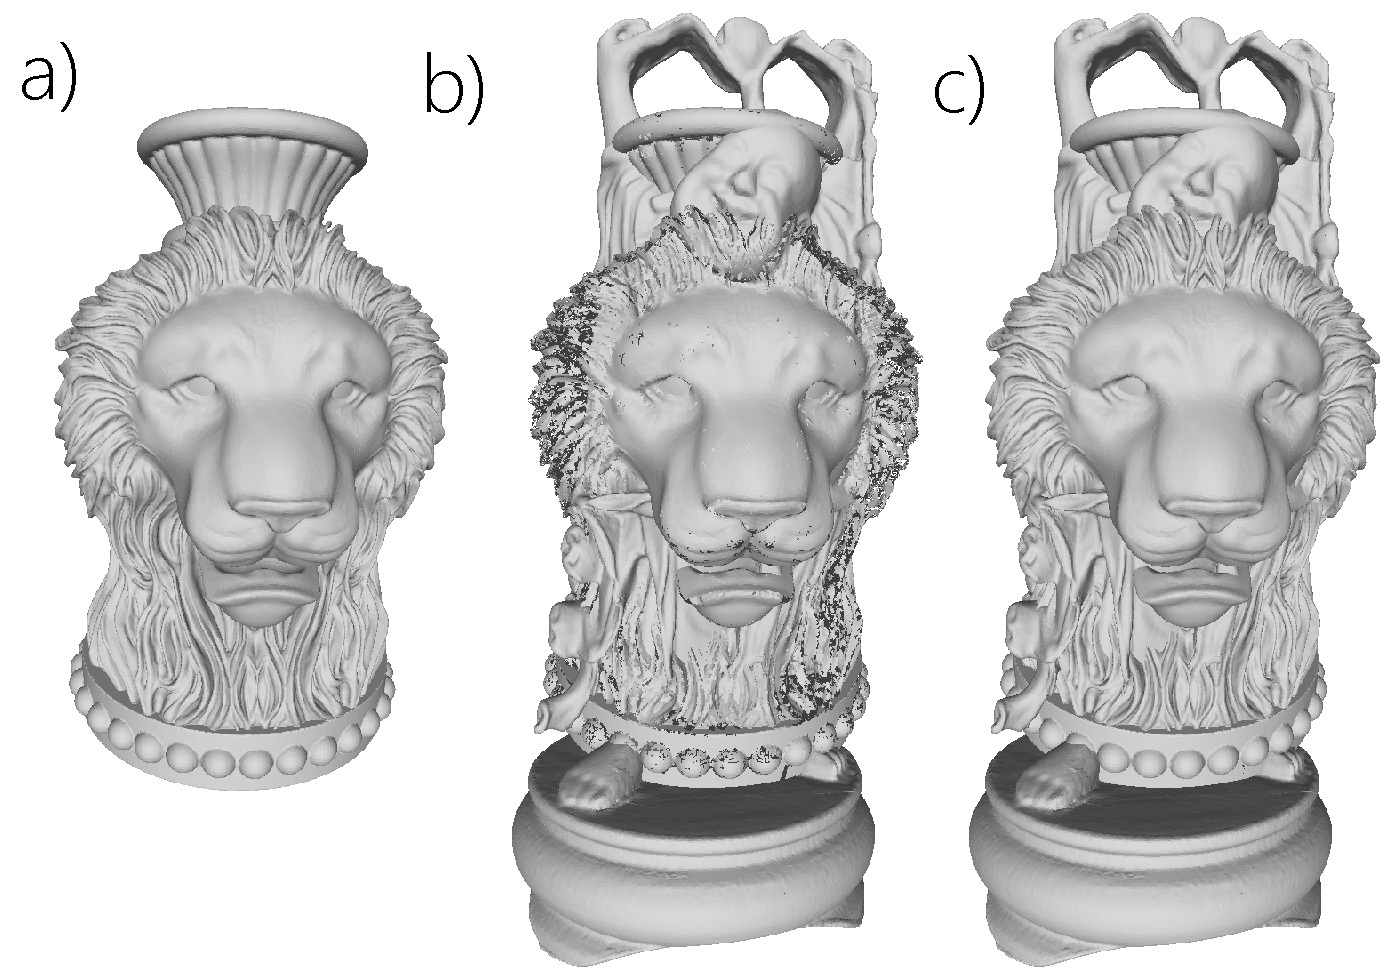
\includegraphics[width=3in]{buddalion}
\caption{ Results from $Budda\cup Lion$: a) incorrect result using CGAL, b) incorrect result using Cork, and c) correct result using our method. }
%.
\label{fig:buddalion}
\end{figure}

%We implemented the proposed method in C++ and tested a series of models on a laptop with Intel Core i5 1.5GHz CPU and 8GB RAM. To prove both the efficiency and robustness, we perform boolean evaluation on various CSGs with different complexity. We also compared our method with several previous works with available implementations, including CGAL \cite{cgal:hk-bonp3-15a}, Maya \cite{Maya2015,barki2015exact},"Cork" \cite{Cork}, "QuickCSG" \cite{douze2015quickcsg}, "Carve" \cite{Carve}, and online service of Campen and Kobbelt's plane-based method \cite{campen2010exact,WebBSP}.

We implemented our proposed method in C++, and tested a series of models on a laptop with an Intel Core i5 1.5 GHz CPU and 8 GB of RAM. To validate the efficiency and robustness of our method, we performed boolean evaluations on various CSGs with different complexities. We also compared our method with several existing methods, including CGAL \cite{cgal:hk-bonp3-15a}, Maya \cite{Maya2015,barki2015exact}, Cork  \cite{Cork}, QuickCSG \cite{douze2015quickcsg}, Carve \cite{Carve}, and online implementations of Campen and Kobbelt��s plane-based method \cite{campen2010exact,WebBSP}.



\subsection{Robustness \& Performance}



\begin{figure}[t]
\centering
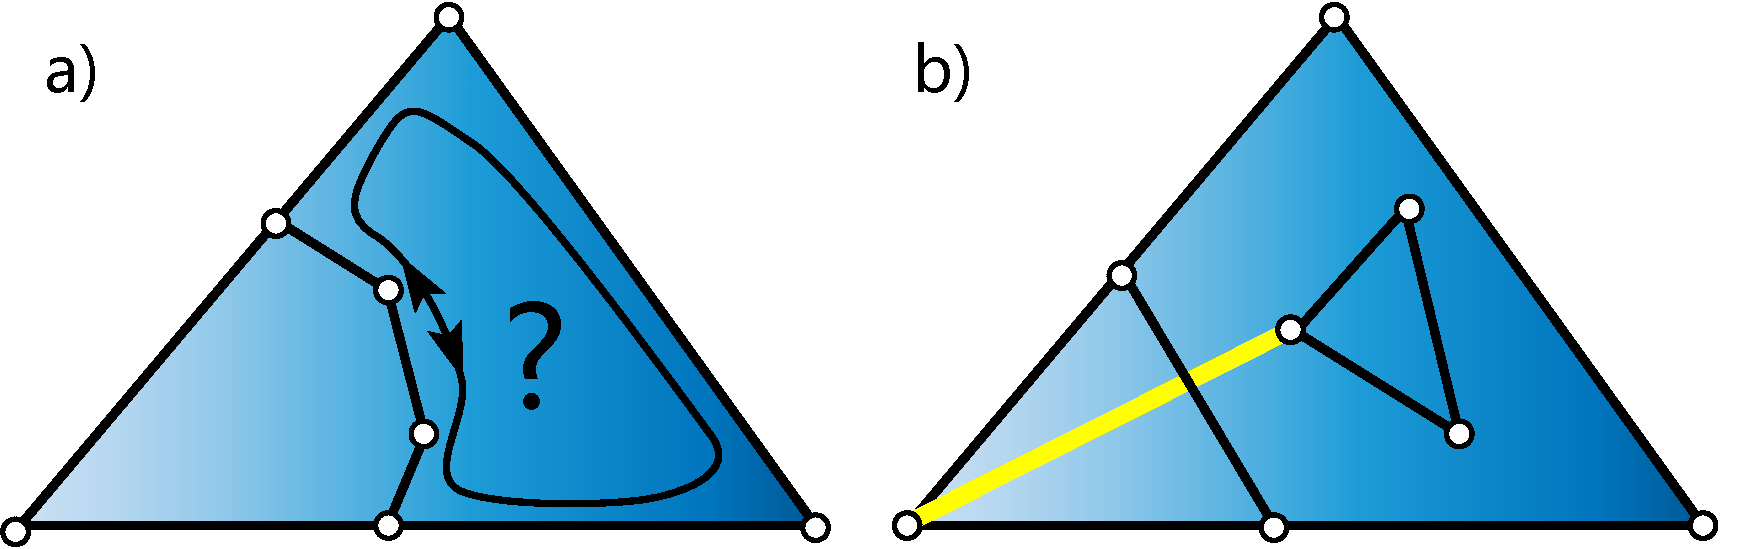
\includegraphics[width=3in]{dual}
\caption{a) There is ambiguity as to the orientation of the loop in this tess-graph. b) When there is more than one connected component in a tess-graph, auxiliary intersections (yellow line) are used to connect the components.}
%a) There is ambiguity with the orientation of the loop in a tess-graph. b) When there are more than one connected component in tess-graph, we use auxiliary intersection (yellow line) to connect the two component. }
\label{fig:dual}
\end{figure}



\begin{table*}[ht]
\caption{Results of self-union evaluation using different methods}
\label{tab:selfunion}
\centering
\begin{tabular}{*{8}{c|}c}%*{4}{>{\centering\arraybackslash}p{35pt}}}
\hline
{No.} & {Model} & {Face Num.} &
CGAL & Maya & Cork & Carve & QuickCSG  & Our Method
\\
\hline\hline
1 & Ball & 360  & \cmark & \cmark & \xmark & \cmark & \xmark & \cmark \\
2 & Head & 2.7k& \cmark & \cmark & \xmark & \cmark & \xmark  & \cmark\\
3 & Bunny & 70k  & \xmark & \cmark & \xmark & \cmark & \xmark  & \cmark\\
4 & Dragon & 277k & \xmark & \xmark & \xmark & \xmark & \xmark  & \cmark \\
\hline
\end{tabular}
\begin{flushleft}
\end{flushleft}
\end{table*}

\begin{table*}[ht]
\caption{Computation time statistics of binary boolean operations (seconds)}
\label{tab:performance}
\centering
\begin{tabular}{*{9}{c|}c}%*{4}{>{\centering\arraybackslash}p{35pt}}}
\hline
{No.} & {Model} & {Face Num. 1} & {Face Num. 2} &
CGAL & Maya & Cork & Carve & QuickCSG & Our Method
\\
\hline\hline
1 & Budda $\cup$ Lion & 1.08M & 400k & - & - & - & - & 3.44 & 6.88\\
2 & Dragon $\cup$ Bunny & 100k & 70k & - & - & - & - & 0.613 &1.70 \\
3 & Armadillo $\cup$ Armadillo2 & 150k & 150k & 487 & 15.4 & 7.00 & 189 & 0.746 & 1.62\\
4 & Horse $\cup$ Corpse & 145k & 499k & - & 38.6 & 12.6 & 1.52k & 0.630 & 1.00 \\
5 & Budda $\cup$ Budda2 & 1.08M & 1.08M & - & - & - & - & 4.84 & -\\
\hline
\end{tabular}
\begin{flushleft}

\end{flushleft}
\end{table*}

\begin{table*}[ht]
\caption{Computation time statistics of the evaluations of large CSGs (seconds)}
\label{tab:performance2}
\centering
\begin{tabular}{*{8}{c|}c}%*{4}{>{\centering\arraybackslash}p{35pt}}}
\hline
{No.} & {Model} & {Face Num.} & {Mesh Num.} &
CGAL  & Cork & Carve & QuickCSG & Our Method
\\
\hline\hline
1 & Sprocket & 11k & 52 & 211  & - & 4.26 & 0.132 & 0.804\\
2 & Ring \& Ball & 146k & 801 & -  & - & 187 & - & 62.6\\
3 & T1 & 80k & 50 & 1.00k & 18.5 & 10.4 & 0.388 & 20.2\\
4 & T2 & 7k & 50 & 2.81k & - & 16.0 & 0.804 & -\\
5 & H & 33k & 42 & - & - & - & 2.22 & -\\
6 & Organic & 219k & 6 & - & 14.3 & 63.1 & 0.580 & 2.75\\
%7 & 6 Budda & - & 43 & - & - & - & - & - & -\\
%8 & Serpent & - & 5 & - & - & - & - & - & -\\
\hline
\end{tabular}
\begin{flushleft}
\end{flushleft}
\end{table*}



\vspace{0.5em}
\noindent\textbf{Self-union}~~~~
%Our method is unconditionally robust for regular set mesh inputs. Even extreme degenerate cases will not lead to failure. To prove that, we tested the self-union of several examples. Table \ref{tab:selfunion} shows whether the tested methods gave a valid outputs. The word 'valid' means the outputs are almost the same with the inputs. In fact, the example models \emph{Bunny} and \emph{Dragon} contain topology deficiencies like self-intersection that cannot perform regular set boolean operations. Despite of that, we find that our method works good in all these cases, indicating the robustness of our method. QuickCSG and Cork failed in all cases, because they cannot deal with coplanar faces. By perturbing one of the operant, the results of QuickCSG are visually OK. However, the topology of their results is messy. We can see hundreds of boundary faces on their results which do not exist in the original model (Fig. \ref{fig:boundaryedge}).
Our method is unconditionally robust for regular set mesh inputs, and even extremely degenerate cases will not lead to failure. To prove this, we tested the self-union of several examples. Table . To prove that, we tested the self-union of several examples. Table  shows whether the methods tested gave valid outputs. Here, the word 'valid' means that the outputs are almost the same as the inputs. The example models \emph{Bunny} $\cap$ \emph{Dragon}  contain topological deficiencies, such as self-intersection, that cannot be processed using regular set boolean operations. Despite this, we found that our method gave good results in these cases, indicating the robustness of our method. QuickCSG and Cork failed in all cases, because they cannot process models with coplanar faces. By perturbing one of the operands, the results of QuickCSG appear visually acceptable. However, the topologies of these results are inaccurate. Hundreds of their boundary faces do not exist in the original model (Fig.  \ref{fig:boundaryedge}).


\vspace{0.5em}
\noindent\textbf{Binary boolean operations}~~~~
%The most common situation of CSG evaluation is to perform boolean operations one by one, since many designers are used to modify models progressively. While our method can evaluate multiple boolean operations once for all, we also compared the performance of binary boolean operations to prove the efficiency. Table \ref{tab:performance} shows the evaluation time of different methods. We can clearly see our method is very fast that is only twice as slower than the fastest non-robust QuickCSG. Other robust methods such as Maya and CGAL are much slower because they use the arbitrary precision arithmetic. Moreover, these robust methods have very strict requirements on the inputs and fragile with topology deficiencies. They simply crash when the inputs are not valid, while our method always tries to give an answer. We also noticed that in (some) very large CSGs, most time is spent on octree construction in our method. It means other stages which involve plane-based geometry take only a small percentage of time, which proves the efficiency of our plane-based algorithms*.
The most common process for CSG evaluation is to perform boolean operations in series. Although our method can evaluate multiple boolean operations simultaneously, we compared the performance of binary boolean operations to determine its efficiency. Table \ref{tab:performance} shows the evaluation times of different methods. These results show that  our method is very fast, and that it is half the speed of the fastest non-robust method, QuickCSG. Other robust methods, such as Maya and CGAL, are much slower, because they use arbitrary precision arithmetic. Moreover, these robust methods have very strict requirements for the inputs, and do not always deal well with topological deficiencies. These methods simply fail when the inputs are not valid, while our method always attempts to provide a result. With (some) very large CSGs, our method spends the most time on octree construction. This means the other stages, which involve plane-based geometry, take only a small percentage of the time. This further demonstrates the efficiency of our plane-based algorithms*.

\vspace{0.5em}
\noindent\textbf{CSGs with large number of meshes}~~~~
%To identify the ability of evaluating large CSG, we also test some CSG with tens or hundreds of meshes. Only QuichCSG and our method can perform multiple boolean operations directly, while others have to decompose CSG trees into binary boolean operations.. We see that the computation time of robust methods like CGAL and Maya is unacceptable long for large CSGs. On the other hand, our method keeps good performance and stability. During our experiments, we noticed sometimes Maya gives the correct results in the first few binary boolean operations, but failed in the later ones. It proves a disadvantage of incremental boolean operation methods---it could accumulate numerical errors which affects the algorithm stability.
To identify the ability of the methods to evaluate large CSGs, we tested some CSGs with tens or hundreds of meshes. Only QuichCSG and our method can perform multiple boolean operations directly. Other methods decompose CSG trees into binary boolean operations. The computation times of robust methods like CGAL and Maya were found to be unacceptably long for large CSGs. Conversely,  our method showed good performance and stability. During our experiments, Maya gave the correct results in the first few binary boolean operations, but failed in the later ones. This demonstrates a disadvantage of incremental boolean operation methods��they can accumulate numerical errors which affect the algorithm��s stability.


\begin{figure*}[!t]
\centering
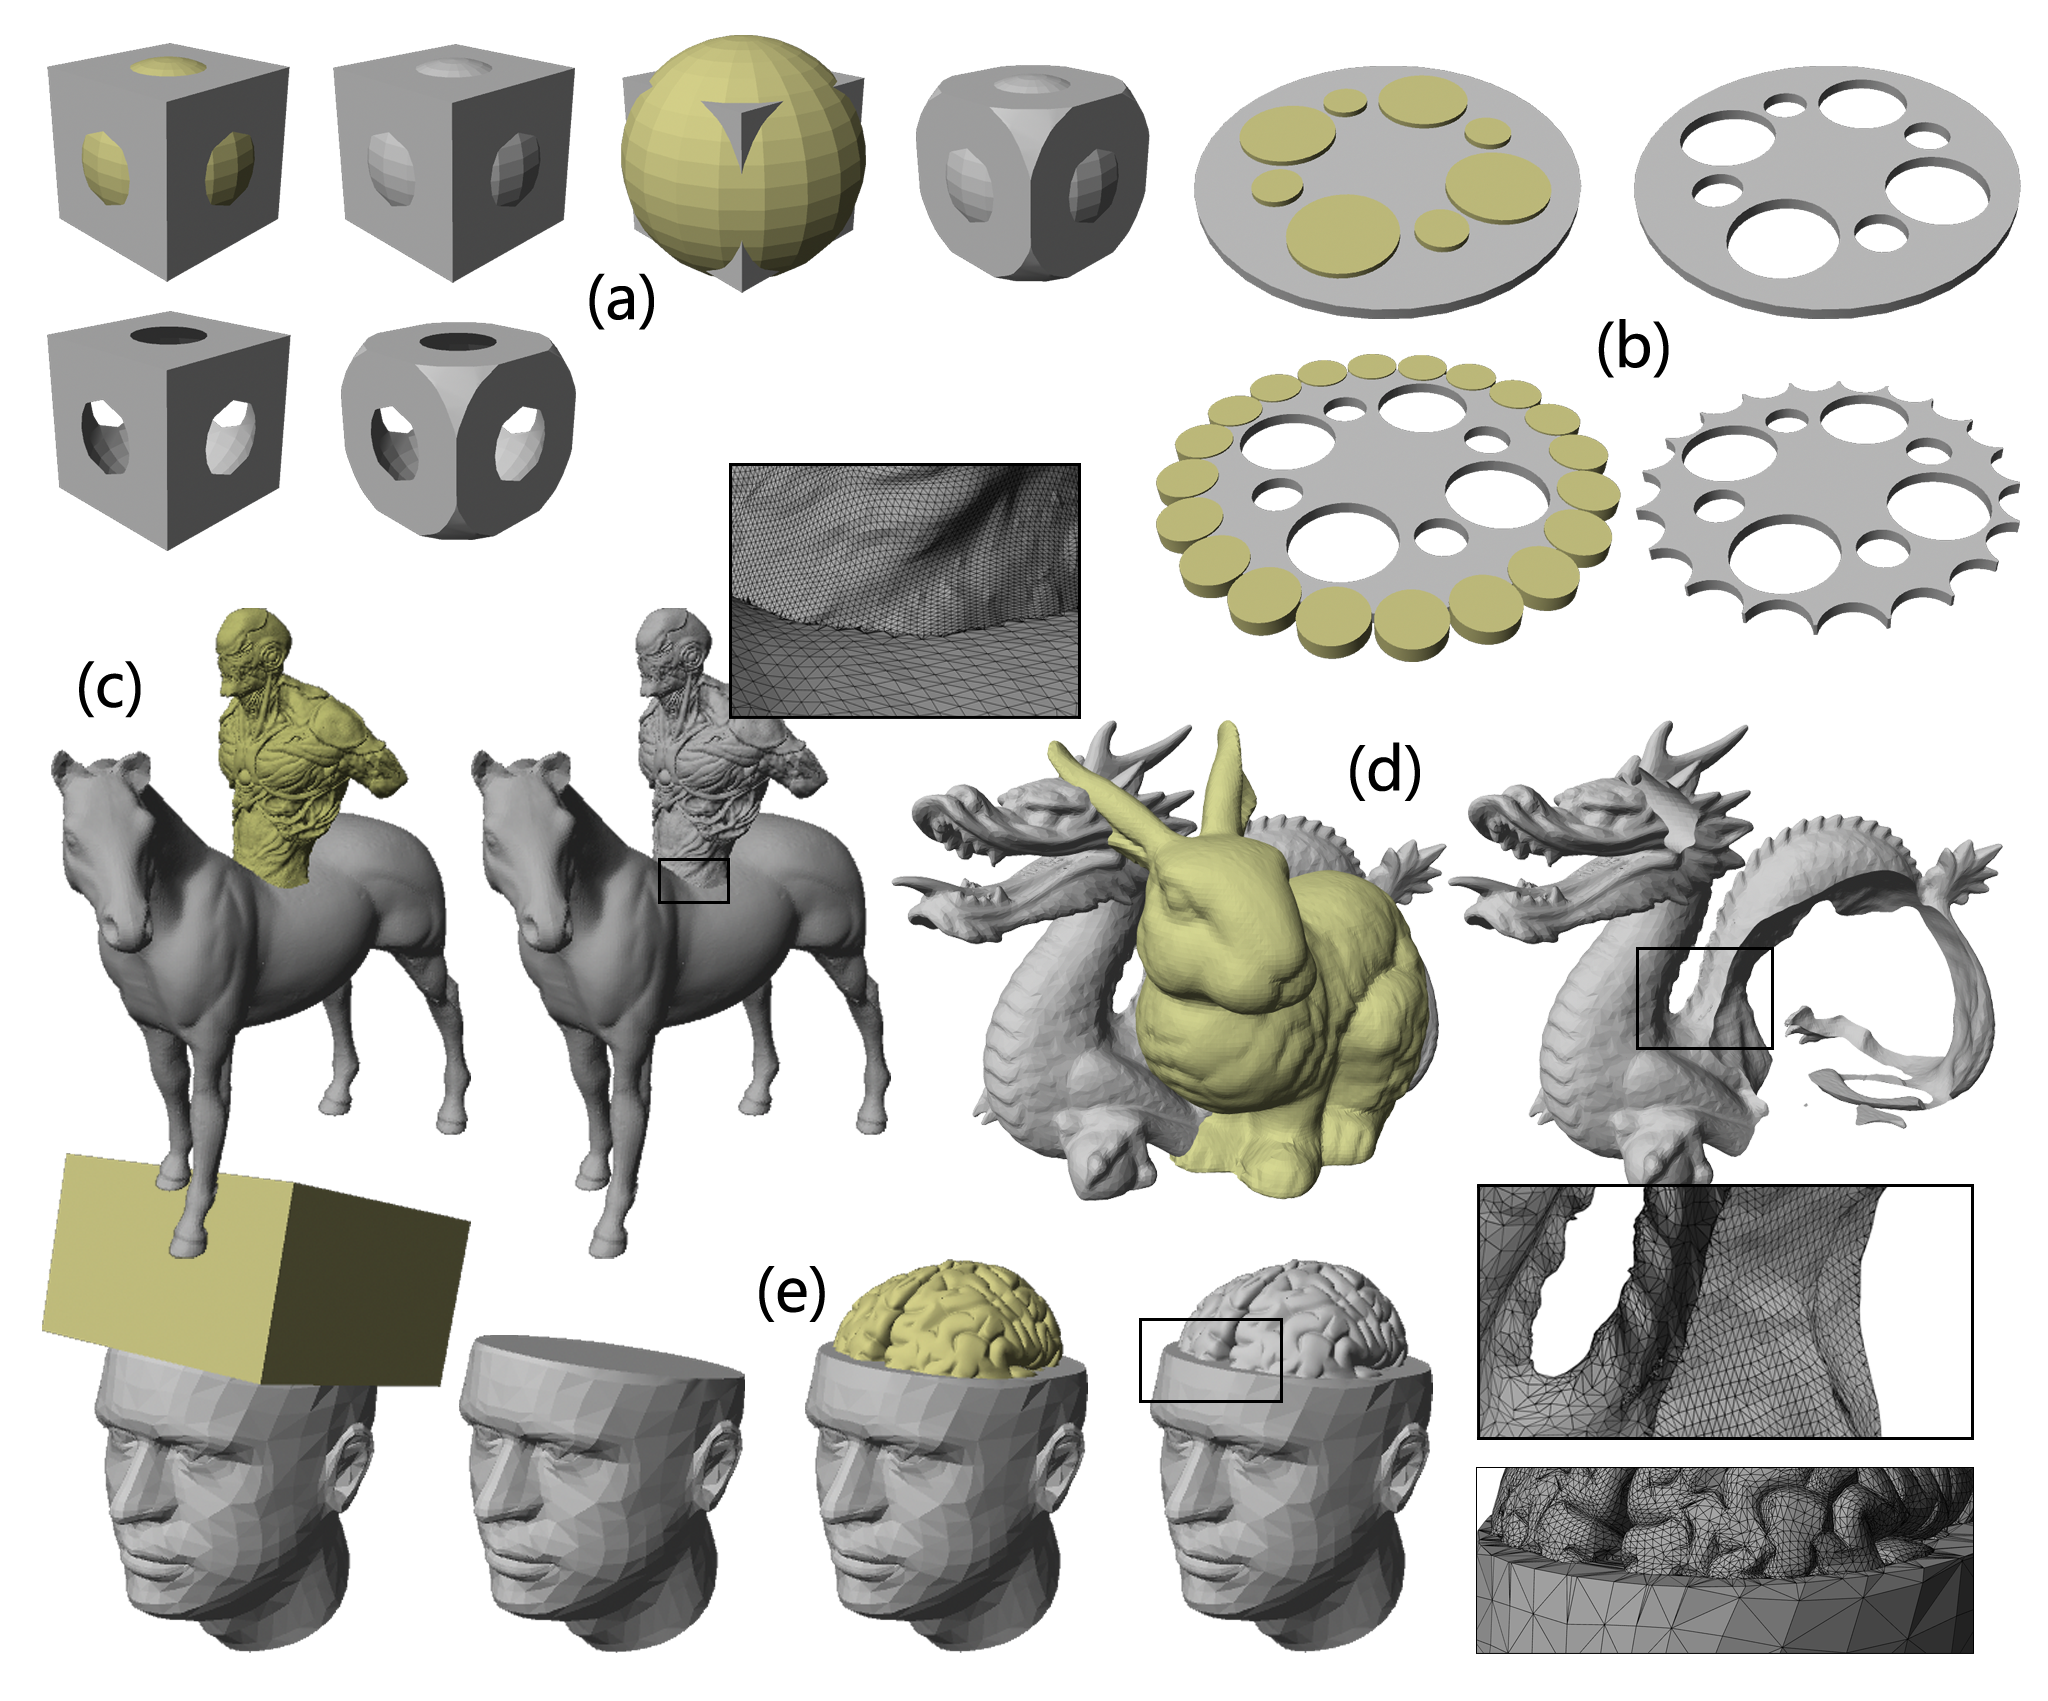
\includegraphics[width=7in]{models}
\caption{***********different models: will be replaced}
\label{fig:models}
\end{figure*}

\subsection{Implementation}
\label{sec:esubroutine}


\vspace{0.5em}
\noindent\textbf{Searching valid loops}~~~~ %In \S\ref{sec:tess}, we claim a valid loops on tess-graph has to be correct with its orientation. However, since tess-graph is undirectional, it is not easy to check whether a loop orientation agrees with the face's (Fig. \ref{fig:dual}a). We observe that the graph connections on the triangle edges have unambiguous directions. Starting from these edges, we can guarantee that the loops have the right orientations. After we find a valid loop, more graph connections will have unambiguous directions because one connection can participate at most two valid loops. In such way, the correct orientation will propagate in a flood-filling way.
Searching valid loops In \S\ref{sec:tess}, we stated that a valid loop on a tess-graph must correspond to its orientation. However, as a tess-graph is nondirectional, it is difficult to check whether a loop orientation agrees with that of the face (Fig. \ref{fig:dual}a). The graph connections on the triangle edges have unambiguous directions. Thus, starting from these edges, we can guarantee that the loops will have the right orientations. After a valid loop is found, more graph connections will have unambiguous directions, because one connection can participate in two valid loops at most. Therefore, the correct orientation will propagate in a flood-filling manner.

\vspace{0.5em}% There is another problem that the tess-graph may not be a connected graph. We avoid this problem by inserting auxiliary intersections into the tess-graph to make it connected. An auxiliary intersection links the corner vertex of triangle face (denoted as $\bm{v}_i$), which is certainly on the outer component, with the vertex on the inner component. The intersection refinement has to be performed again if the auxiliary intersections cross any other intersections. This trick slight obey the principle of no constructions. To guarantee the auxiliary intersection has a valid PBI-rep, we require the vertex from inner connected component generated by intersection between the triangle and an edge (denoted as $\bm{e}_j$) from other meshes---all intersection end points during triangle-triangle intersection are this type. In this way, we get three vertices with exact coordinates ($\bm{v}_i$ and the two end points of $\bm{e}_j$) and can construct an exact plane where the auxiliary intersection lies.
There is no guarantee that the tess-graph will be a connected graph. We solve this problem by inserting auxiliary intersections into the tess-graph, to ensure it is connected. An auxiliary intersection links the corner vertex ( $\bm{v}_i$) of a triangle face which is confirmed to be on the outer component, with the vertex on the inner component. The intersection refinement needs to be performed again if the auxiliary intersections cross any other intersections. This solution is consistent with the principle of no constructions. To guarantee that the auxiliary intersection has a valid PBI-rep, the vertex must be determined from the inner connected component generated by the intersection between the triangle and an edge (denoted as $\bm{e}_j$) from another mesh. All intersection end points of triangle-triangle intersections are of this type. Therefore, we obtain three vertices with exact coordinates ($\bm{v}_i$ and the two end points of $\bm{e}_j$), and, therefore, can construct the plane on which the auxiliary intersection lies.

\vspace{0.5em}
\noindent\textbf{Seed indicator generation}~~~~%In \S\ref{sec:propagation}, we claim that our flood-filling starts from a seed vertex $\bm{v}_0$. While the indicator vector of the seed $\bm{\Lambda}(\bm{v}_0)$ can be generated by point-in-polyhedron test \cite{ogayar2005point} with the octree as acceleration structure \cite{frisken2002simple}, we have simpler strategies by using vertex with known indicators as the seed. We choose the vertex with the max $x$-coordinate as the seed. In this way, its indicators are either $out$ ($in$, if complement is applied on mesh) or $on$. The $on$ indicators are easy to determine in most time. Sometimes exception occurs because of coplanar situation---vertices may not be registered on the mesh even if it is on the mesh. Fortunately, if we carefully choose the right vertex whose neighboring faces are not coplanar, this will not happen.
Seed indicator generation In \S\ref{sec:propagation}, state that flood-filling starts from a seed vertex $\bm{v}_0$. The indicator vector of the seed $\bm{\Lambda}(\bm{v}_0)$ can be generated by a point-in-polyhedron test \cite{ogayar2005point}, using the octree as an acceleration structure \cite{frisken2002simple}. However, a simpler strategy is to use a vertex with known indicators as the seed. The vertex with the maximum $x$-coordinate is chosen as the seed. Its indicators are either $out$ ($in$, if the complement is applied on the mesh) or $on$. The $on$ indicators are generally easy to determine. Exceptions can occur because of coplanar situations��vertices may not be registered on the mesh, even if they are on the mesh. Fortunately, if a vertex is chosen whose neighboring faces are not coplanar, this will be prevented.

\vspace{0.5em} %The indicator vectors can propagate not only among single meshes, but can also between different meshes by the vertices and edges they share. Therefore in most time, we only need one single seed vertex for classification. However, if there are more than two connected components among meshes, we extra seeds to propagate each component. The indicators of the second and later seeds can be computed by point-in-polyhedron tests.
Indicator vectors can propagate among single meshes, and between different meshes across shared vertices and edges. Therefore, in most cases, only a single seed vertex is needed for classification. However, if there are more than two connected components among the meshes, extra seeds are required to propagate each component. The indicators of these additional seeds can be computed by point-in-polyhedron tests.

\vspace{0.5em}
\noindent\textbf{Exporting to float-point number}~~~~
%The vertices of final mesh in our method are represented in either planes or vertex coordinates. While the vertices from the input meshes have there exact coordinates, the vertices newly introduced by intersection between meshes have only P-reps and require round-off when computing coordinates. Though we guarantee the correct topology in the result mesh, such round-off can still cause topology deficiencies. Here we adopt Zhou et al.'s method \cite{zhou2016mesh} to solve it iteratively.
Exporting to float-point number The vertices of the final mesh generated by our method are represented as either planes or vertex coordinates. The vertices originating from the input meshes have exact coordinates, however, the vertices newly introduced by the intersection between meshes have only P-reps, and require rounding-off when computing their coordinates. Although our method guarantees the correct topology in the final mesh, rounding errors can cause topological deficiencies. The method of Zhou et al. \cite{zhou2016mesh} can be used to solve this problem iteratively.

\subsection{Limitations and Future Work}

%We noticed that for CSGs that contains a lot of meshes within small area (e.g., Table. \ref{tab:performance}, \emph{T1}), the performance of our method is poor. This is because in such situations, our method computes many intersections that will not appear as edges in the final mesh, which leads to unnecessary tessellation. Optimization may be explored to avoid such problem.

%The input of our method is limited to regular set meshes. However, recent works claim that the piece-wise wind number (PWN) are more powerful to identify the inside and outside of meshes \cite{zhou2016mesh}.  By using PWN, the input requirements can be extended to so-called PWN meshes that allow topology deficiencies such as self-intersection and multi-component. It would be interesting to extend our method to PWN method in the future.

We found that performance of our method was poor for CSGs that contained a lot of meshes within a small area (Table. \ref{tab:performance}, \emph{T1}). In these cases, our method computes many intersections that will not appear as edges in the final mesh, leading to unnecessary tessellation. Optimization may be explored to minimize this problem.

The application of our method is limited to regular set meshes. However, recent reports have proposed that the piece-wise wind number (PWN) is a more powerful method to identify the insides and outsides of meshes \cite{zhou2016mesh}. The input requirements of our method may be extended to PWN meshes, that allow topological deficiencies, such as self-intersection and multi-components. We believe that this would be an interesting and valuable extension of our work.



\section{Summary}

%In this paper, we proposed a novel method to evaluate CSG models. It is able to efficiently perform unconditionally robust non-incremental boolean operations. The key idea of our approach is to embed P-reps information into B-reps. The P-reps give us the chance to strictly follow the principle of no geometry construction to avoid numerical errors. And the B-reps offer fast neighborhood query to accelerate the processing. Experiments have verified the performance of our method is competitive with state-of-the-art non-robust methods while guarantee robustness.

In this paper, we propose a novel method to evaluate CSG models. This method can efficiently perform unconditionally robust non-incremental boolean operations. The novel component of our approach is to embed P-rep information into B-reps. P-reps allow us to strictly follow the principle of no geometry construction to avoid numerical errors. The use of B-reps enables fast neighborhood queries to reduce the computation time. The experimental results show that the performance of our method is competitive with state-of-the-art non-robust methods, while guaranteeing robustness.



\appendices


%\newpage
\bibliographystyle{IEEEtran}
\bibliography{IEEEabrv,citation}


%\newpage

\begin{IEEEbiography}[{\includegraphics[width=1in,height=1.25in,clip,keepaspectratio]{rui}}]{Rui Wang}
is currently a postgraduate student at the Department of Computer Science and Technology, the Shanghai Jiao Tong University. His main research interests include real-time computer graphics and virtual reality applications.
\end{IEEEbiography}

% if you will not have a photo at all:
\begin{IEEEbiography}[{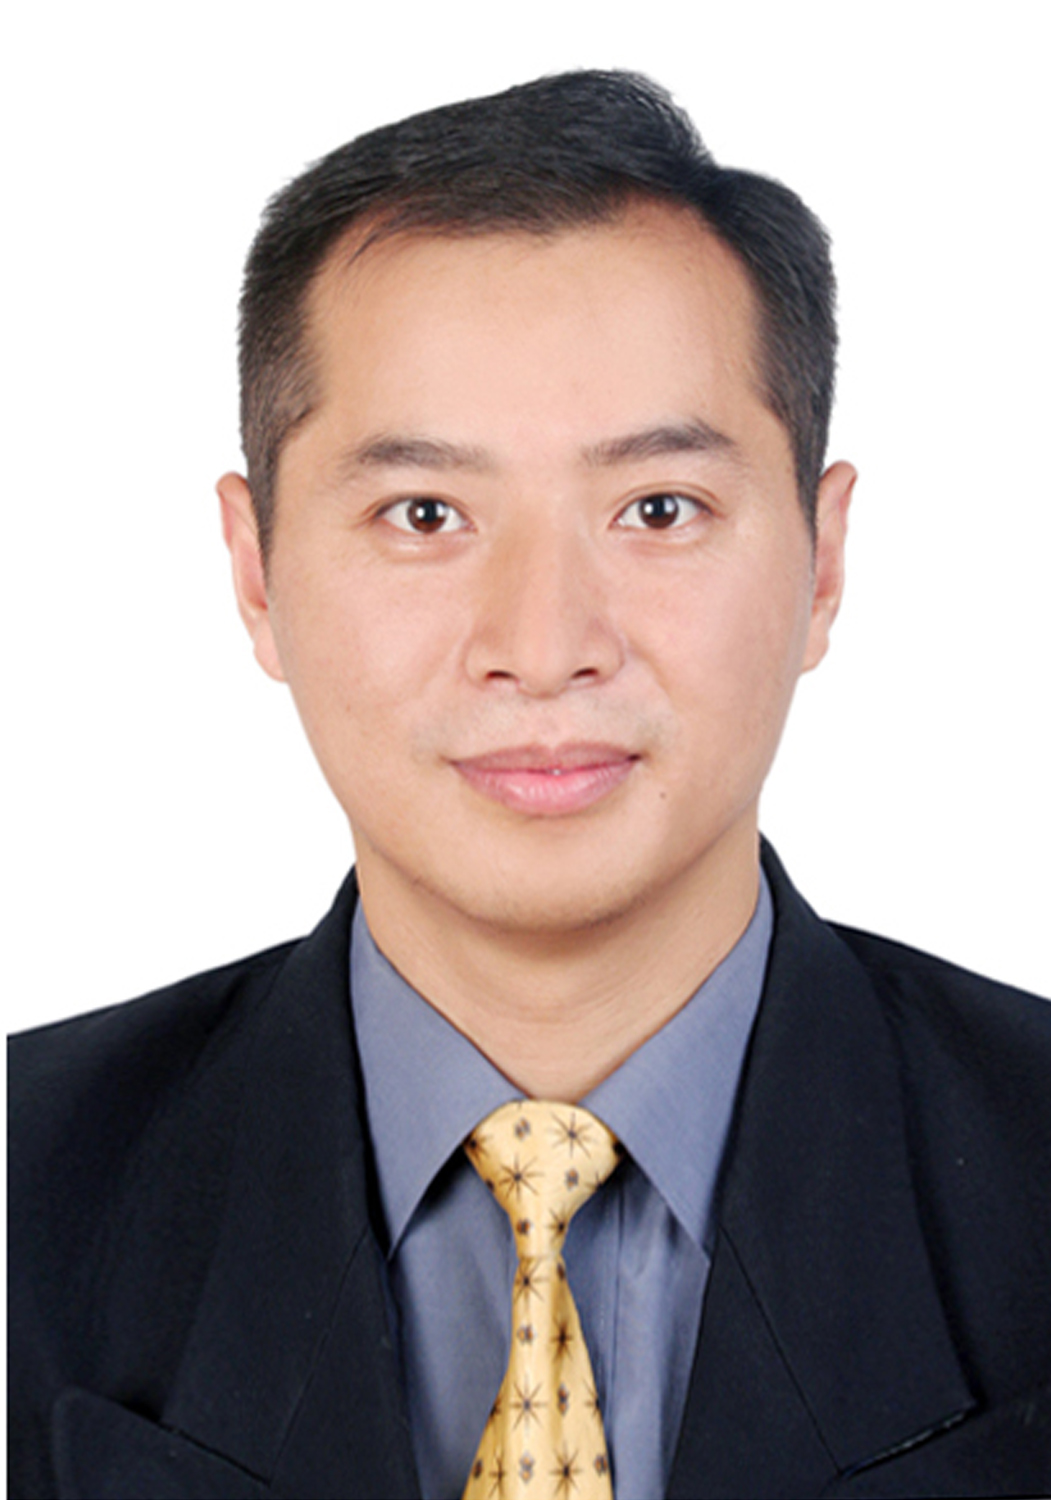
\includegraphics[width=1in,height=1.25in,clip,keepaspectratio]{xudong}}]{Xudong Jiang}
received his Master degree in Computer Science from Shanghai Jiao Tong University in 2014. He is currently working in Autodesk China Research \& Development Center. His research interest includes computer-aided geometric design and solid modeling.
\end{IEEEbiography}


\begin{IEEEbiography}[{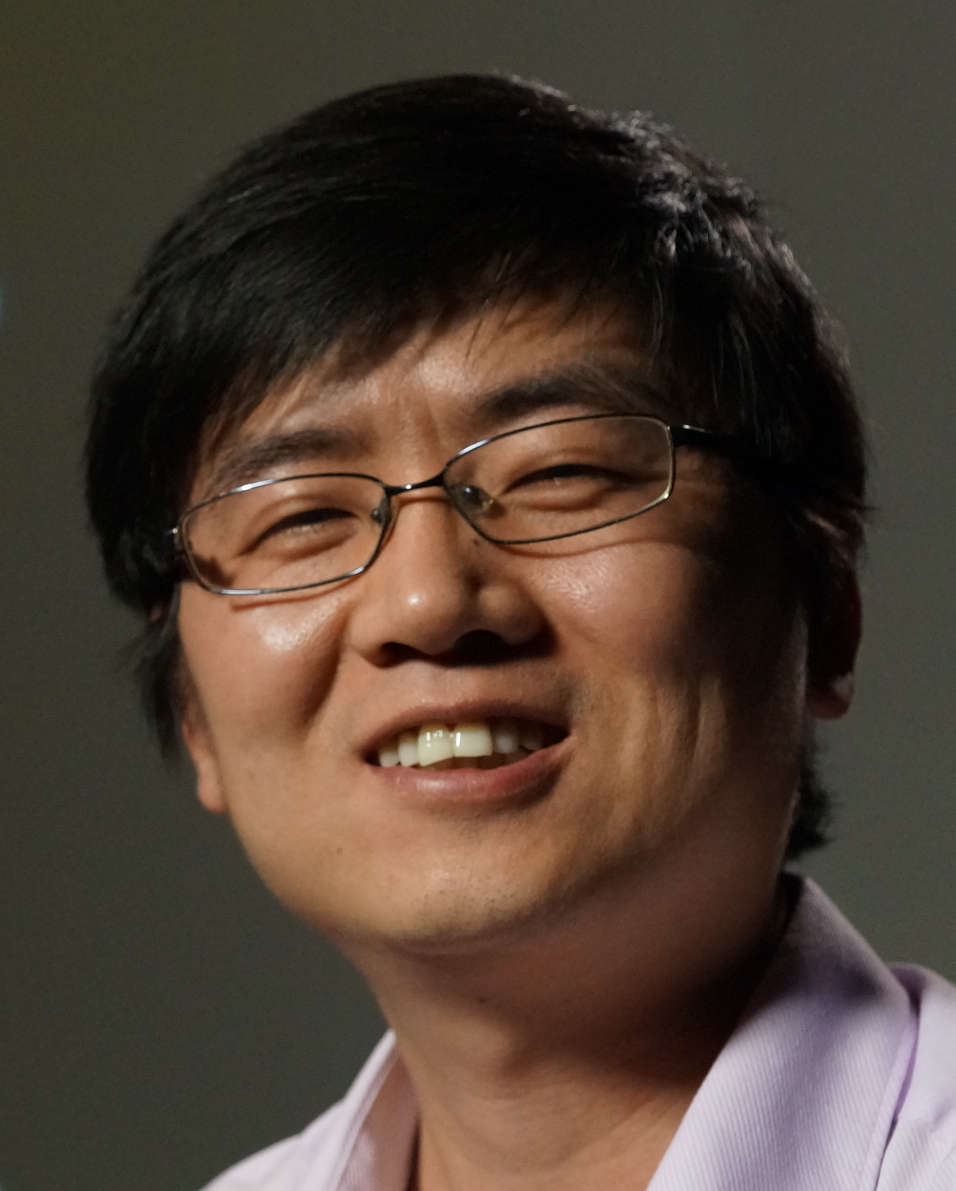
\includegraphics[width=1in,height=1.25in,clip,keepaspectratio]{hongbo}}]{Hongbu Fu}
is an Associate Professor in the School of Creative Media, City University of Hong Kong. He received the PhD degree in computer science from the Hong Kong University of Science and Technology in 2007 and the BS degree in information sciences from Peking University, China, in 2002. His primary research interests fall in the fields of computer graphics and human computer interaction. He has served as an associate editor of The Visual Computer, Computers \& Graphics, and Computer Graphics Forum.
\end{IEEEbiography}


\begin{IEEEbiography}[{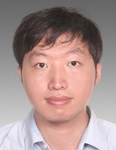
\includegraphics[width=1in,height=1.25in,clip,keepaspectratio]{sheng}}]{Bin Sheng}
received his BS degree in computer science from Huazhong University of Science and Technology in 2004, MS degree in software engineering from University of Macau in 2007, and PhD Degree in computer science from The Chinese University of Hong Kong in 2011. He is currently an associate professor in the Department of Computer Science and Engineering at Shanghai Jiao Tong University. His research interests include virtual reality, computer graphics, and image-based techniques.
\end{IEEEbiography}

\begin{IEEEbiography}[{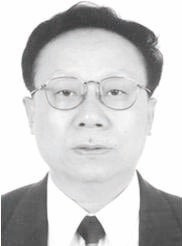
\includegraphics[width=1in,height=1.25in,clip,keepaspectratio]{wu}}]{Enhua Wu}
received the BS degree from Tsinghua University in 1970, and the PhD degree from the University of Manchester (UK) in 1984. He is currently a research professor at the Institute of Software, Chinese Academy of Sciences, and Fellow of China Computer Federation. He has also been teaching at the University of Macau since 1997, where he is currently an Emeritus Professor. His research interests include realistic image synthesis, virtual reality, and scientific visualization. He has served as an associate editor of The Visual Computer, Computer Animation and Virtual Worlds.
\end{IEEEbiography}





\end{document}
